% ============================================================
% This work is published under a CC BY-SA license 
% (Creative Commons Attribution-ShareAlike 4.0 International 
% License), which means that you can copy, redistribute, remix,
% transform, and build upon the content for any purpose, even
% commercially, as long as you give appropriate credit, provide 
% a link to the license, and indicate if changes were made. 
%
% License details: creativecommons.org/licenses/by-sa/4.0 .
% ============================================================

\documentclass[spanish,twoside,openright,10pt]{book}

% preambulo
% ------------------------------------
% paquetes de formato

% paquetes basicos
\usepackage[utf8]{inputenc}
\usepackage[spanish]{babel}

%\usepackage{epsfig}
\usepackage{graphicx}
\usepackage{epstopdf}

\usepackage{amssymb,amsmath,amsfonts,amsthm}%,stmaryrd,latexsym,bbold,psfrag,fontenc,dsfont}
\usepackage{bm}
\usepackage{float}
\usepackage{booktabs}
\usepackage{lscape}
\usepackage{wrapfig}

% color
\usepackage[usenames]{color}
\color{black} % el paquete color define el color por defecto Black cmyk 0 0 0 1 que no es totalmente negro
\usepackage[skins]{tcolorbox}

\usepackage{subfig}

\usepackage{hyphenat}
%\usepackage[hidelinks,bookmarks=false]{hyperref}
\usepackage[plainpages=false]{hyperref}

% diagramacion de hoja
\usepackage[a5paper,top=16.5mm,bottom=12.5mm,left=16.5mm,right=12.5mm,portrait]{geometry}

%\usepackage[cam,a4,center]{crop}
\usepackage[frame,a4,center]{crop}

% fuente
\usepackage{libertine}
\usepackage{libertinust1math}
\usepackage[T1]{fontenc}
% ------------------------------------


% -----------------------------
% estilo de bibliografia
\usepackage{natbib}
\bibliographystyle{../bib/apalike-es}
%\bibliographystyle{apalike}
% -----------------------------

% ----------------------------------------------------
% ----- encabezados ------------
\usepackage{fancyhdr,fancybox}

\pagestyle{fancy}

% with this we ensure that the chapter and section headings are in lowercase.
\renewcommand{\chaptermark}[1]{\markboth{\chaptername\ \thechapter.\hspace{1ex}#1}{}}
\renewcommand{\sectionmark}[1]{\markright{Sección \thesection.\hspace{1ex}#1}}
\fancyhf{} % delete current header and footer
\fancyhead[LE,RO]{\small\sffamily\bfseries\thepage}
\fancyhead[LO]{\small\sffamily\bfseries\nouppercase{\rightmark}}
\fancyhead[RE]{\small\sffamily\bfseries\nouppercase{\leftmark}}
\renewcommand{\headrulewidth}{0.6pt}
\renewcommand{\footrulewidth}{0pt}
\addtolength{\headheight}{3.6pt} % space for the rule
\fancypagestyle{plain}{%
	\fancyhead{} % get rid of headers on plain pages
	\renewcommand{\headrulewidth}{0pt} % and the line
}
% ----------------------------------------------------


\usepackage[normalem]{ulem}
\usepackage[labelfont={small,sf,bf}]{caption}
\usepackage{enumitem}

% para setear interlineado
\usepackage{setspace}

% --------------------------------
% ----- algoritmos y codigos -----

% algoritmos-pseudocodigos
\usepackage{algorithmic}
\usepackage{algorithm}
%\usepackage{algcompatible} %\usepackage{algpseudocode}
\makeatletter
\renewcommand*{\ALG@name}{Algoritmo}
\makeatother
% ----------------------

% marca de agua: EN REVISION
\usepackage[printwatermark]{xwatermark}
\newwatermark[pages=1-200,color=red!10,angle=45,scale=2.0,xpos=0,ypos=0]{En revisión.}


% ----------------------
% codigos embebidos
\usepackage[numbered,framed]{matlab-prettifier}
%
\let\ph\mlplaceholder % shorter macro
\lstMakeShortInline"

\lstset{
	style              = Matlab-editor,
	basicstyle         = \footnotesize\mlttfamily,
	language           = Octave,
	escapechar         = ",
	mlshowsectionrules = true,
}
\renewcommand\lstlistingname{Código}
% ----------------------



% ----------------------------------------------
% seteos varios
% ----------------------------------------------

\usepackage{bigfoot} % to allow verbatim in footnote

\usepackage{titlesec}
\usepackage{titletoc}

%\titleformat{\chapter}[display]{\Huge\sffamily\bfseries}{\chaptertitlename~\thechapter}{2ex}{}
\titleformat{\section}   {\large\sffamily\bfseries}{\thetitle.}{1ex}{}
\titleformat{\subsection}{\small\sffamily\bfseries}{\thetitle.}{1ex}{}
\titleformat{\subsubsection}{\small\sffamily\bfseries}{}{1ex}{}

\titlecontents{chapter}[1.3em]
{\vspace{1.1em}\sffamily\bfseries}
{\contentslabel{1.3em}}
{\hspace*{-1.3em}}
{\titlerule[1pt]\contentspage}
\titlecontents{section}[3.5em]
{\small\sffamily} % note that 3.5 = 1.3 + 2.2
{\contentslabel{2.2em}}
{\hspace*{-2.2em}}
{\titlerule*[1pc]{.}\contentspage}
\titlecontents{subsection}[6.4em]
{\small\sffamily} % note that 6.4 = 3.5 + 2.9
{\contentslabel{2.9em}}
{\hspace*{-2.9em}}
{\titlerule*[1pc]{.}\contentspage}

% --------------------------------------------------------
% Cuadros en ejemplos y ejercicios
% -------------------------------------------------------
\usepackage{framed}

\renewcommand{\FrameCommand}{\shadowbox}

\definecolor{shadecolor}{rgb}{0.8,0.8,0.8}

\setlength{\fboxsep}{0.5em}
%\setlength{\FrameSep}{0.0mm}
%\setlength{\FrameRule}{1pt}
% --------------------------------------------------------

%
\usepackage{pdfpages}



% ----------   paquetes para diagrama de flujo apendice ------------
\usepackage{pgf,tikz}
\usetikzlibrary{arrows,backgrounds,shapes.geometric,calc}
%\usetikzlibrary{arrows,snakes,backgrounds,shapes.geometric,calc}
\listfiles
% -------------------------------------


\usepackage{relsize}

\usetikzlibrary{arrows.meta}
\tikzset{%
	>={Latex[width=2mm,length=2mm]},
	% Specifications for style of nodes:
	base/.style = {rectangle, rounded corners, draw=black,
		minimum width=4cm, minimum height=1cm,
		text centered, font=\sffamily},
	activityStarts/.style = {base, fill=blue!30},
	startstop/.style = {base, fill=red!30},
	activityRuns/.style = {base, fill=green!30},
	process/.style = {base, minimum width=2.5cm, fill=orange!15,
		font=\ttfamily},
}


% esto resuelve problema tikz con babel
\usepackage{etoolbox}
\AtBeginEnvironment{tikzpicture}{\shorthandoff{>}\shorthandoff{<}}{}{}



%
% --------------------------------------------------------
% para figuras con tikz e inkscape

\newcommand*\circled[1]{\tikz[baseline=(char.base)]{
		\node[shape=circle,draw,inner sep=2pt] (char) {#1};}}

% Comandos figuras inkscape
%\newcommand{\executeiffilenewer}[3]{%
%\ifnum\pdfstrcmp{\pdffilemoddate{#1}}%
%{\pdffilemoddate{#2}}>0%
%{\immediate\write18{#3}}\fi%
%}
%\newcommand{\includesvg}[1]{%
%\executeiffilenewer{#1.svg}{#1.pdf}%
%{inkscape -z -D --file=#1.svg %
%--export-pdf=#1.pdf --export-latex}%
%\input{#1.eps_tex}%
%}

% agrega ruta a figuras
\graphicspath{{../fig/}}
% -------------------------------------------
%
%
\newtheoremstyle{miestilo}% <name>
{0pt}% <Space above>
{0pt}% <Space below>
{\normalfont}% <Body font>
{0pt}% <Indent amount>
{\small\sffamily\bfseries}% <Theorem head font>
{\quad}% <Punctuation after theorem head>
{0pt}% <Space after theorem head>
{}% <Theorem head spec (can be left empty, meaning `normal')>

\addto{\captionsspanish}{\renewcommand*{\tablename}{Tabla}}

\theoremstyle{miestilo}
\newtheorem{SHteorema}{Teorema}[chapter]
\newtheorem{SHcorolario}[SHteorema]{Corolario}
\newtheorem{SHhipotesis}[SHteorema]{Hipótesis}
\newtheorem{SHlema}[SHteorema]{Lema}
\newtheorem{SHnotacion}[SHteorema]{Notación}
\newtheorem{SHdefinicion}[SHteorema]{Definición}
\newtheorem{SHejemplo}[SHteorema]{Ejemplo}
\newtheorem{SHejercicio}[SHteorema]{Ejercicio}
\newtheorem{SHobservacion}[SHteorema]{Observación}
\newtheorem{axioma}{Axioma}
%
\newenvironment{teorema}[1][]{\begin{SHteorema}[#1]\begin{framed}}{\end{framed}\end{SHteorema}}
\newenvironment{corolario}[1][]{\begin{SHcorolario}[#1]\begin{framed}}{\end{framed}\end{SHcorolario}}
\newenvironment{hipotesis}[1][]{\begin{SHhipotesis}[#1]\begin{framed}}{\end{framed}\end{SHhipotesis}}
\newenvironment{lema}[1][]{\begin{SHlema}[#1]\begin{framed}}{\end{framed}\end{SHlema}}
\newenvironment{definicion}[1][]{\begin{SHdefinicion}[#1]\begin{framed}}{\end{framed}\end{SHdefinicion}}
\newenvironment{notacion}[1][]{\begin{SHnotacion}[#1]\begin{framed}}{\end{framed}\end{SHnotacion}}
\newenvironment{ejemplo}[1][]{\begin{SHejemplo}[#1]\begin{framed}}{\end{framed}\end{SHejemplo}}
\newenvironment{ejercicio}[1][]{\begin{SHejercicio}[#1]\begin{framed}}{\end{framed}\end{SHejercicio}}
\newenvironment{observacion}[1][]{\begin{SHobservacion}[#1]\begin{framed}}{\end{framed}\end{SHobservacion}}

\newcommand{\subtitulo}[1]{~\\\noindent{\small\sffamily\bfseries #1}\vspace{2mm}}

\usepackage{lineno}

%\definecolor{miblue}{rgb}{0,0.1,0.5}%
\definecolor{miblue}{rgb}{0,0.1,0.38}%
%
\definecolor{colorbordecajas}{rgb}{0,0.1,0.4}%
\definecolor{colorfondocajas}{rgb}{.86,.91,.996}%
%
%
% -----------  cajas ----------------------------
\newcommand{\cajaactividad}[1]{
\begin{center}
\begin{tcolorbox}[enhanced,width=0.9\textwidth,drop fuzzy shadow southwest,colframe=colorbordecajas,colback=colorfondocajas,title=\textbf{Actividad}]
#1
\end{tcolorbox}
\end{center}
}

\definecolor{colorbordecajasconcepto}{rgb}{0.1,0.33,0.01}%
%\definecolor{colorfondocajasconcepto}{rgb}{.73,.95,.65}%
\definecolor{colorfondocajasconcepto}{rgb}{.9,.99,.8}%

\newcommand{\cajaconcepto}[2]{
	\begin{center}
		\begin{tcolorbox}[enhanced,width=0.9\textwidth,drop fuzzy shadow southwest,colframe=colorbordecajasconcepto,colback=colorfondocajasconcepto,title=\textbf{#1}]
			#2
		\end{tcolorbox}
	\end{center}
}
% ---------------------------------------------------------
%
%
\titleformat{\chapter}
{\normalfont\Large\color{miblue}\bfseries}{\color{miblue}\chaptername\ \thechapter:}{1em}{}[{\color{miblue}\titlerule[0.8pt]}]


%\usepackage{forest}

%\definecolor{foldercolor}{RGB}{124,166,198}
%
%\tikzset{pics/folder/.style={code={%
%			\node[inner sep=0pt, minimum size=#1](-foldericon){};
%			\node[folder style, inner sep=0pt, minimum width=0.3*#1, minimum height=0.6*#1, above right, xshift=0.05*#1] at (-foldericon.west){};
%			\node[folder style, inner sep=0pt, minimum size=#1] at (-foldericon.center){};}},
%	pics/folder/.default={20pt},folder style/.style={draw=foldercolor!80!black,top color=foldercolor!40,bottom color=foldercolor}
%}
%
%\forestset{is file/.style={edge path'/.expanded={%
%			([xshift=\forestregister{folder indent}]!u.parent anchor) |- (.child anchor)},
%		inner sep=1pt}, this folder size/.style={edge path'/.expanded={%
%			([xshift=\forestregister{folder indent}]!u.parent anchor) |- (.child anchor) pic[solid]{folder=#1}}, inner ysep=0.6*#1},
%	folder tree indent/.style={before computing xy={l=#1}},
%	folder icons/.style={folder, this folder size=#1, folder tree indent=3*#1},
%	folder icons/.default={12pt},
%}



% archivo de definiciones
% ---- Some commands definitions file for latex -------

% --- nombres propios ---
\def\Tikhonov{Tikhonov} 
\def\Young{Young}
\def\Poisson{Poisson}
\def\Cauchy{Cauchy}

\def\bbA{{\mathbb A}} 
\def\bbB{{\mathbb B}} 
\def\bbC{{\mathbb C}} 
\def\bbE{{\mathbb E}} 
\def\bbF{{\mathbb F}} 
\def\bbI{{\mathbb I}} 
\def\bbL{{\mathbb L}} 
\def\bbN{{\mathbb N}} 
\def\bbP{{\mathbb P}} 
\def\bbQ{{\mathbb Q}} 
\def\bbR{{\mathbb R}} 
\def\bbS{{\mathbb S}}
\def\bbT{{\mathbb T}}

% Text colors
\def\tr[#1]{\textcolor{red}{#1}}
\def\tg[#1]{\textcolor{green}{#1}}
\def\tb[#1]{\textcolor{blue}{#1}}
% -----------


% --------- mathcal ------
\def\mcA{{\mathcal A}}
\def\mcC{{\mathcal C}}
\def\mcD{{\mathcal D}}
\def\mcE{{\mathcal E}}
\def\mcF{{\mathcal F}}
\def\mcG{{\mathcal G}}
\def\mcH{{\mathcal H}}
\def\mcI{{\mathcal I}}
\def\mcJ{{\mathcal J}}
\def\mcK{{\mathcal K}}
\def\mcN{{\mathcal N}}
\def\mcO{{\mathcal O}}
\def\mcP{{\mathcal P}}
\def\mcR{{\mathcal R}}
\def\mcS{{\mathcal S}}
\def\mcU{{\mathcal U}}
\def\mcV{{\mathcal V}}
\def\mcX{{\mathcal X}}
\def\mcW{{\mathcal W}}

% math operators
\DeclareMathOperator{\sgn}{sgn}
\DeclareMathOperator{\sym}{sym}
\DeclareMathOperator{\Grad}{Grad}
\DeclareMathOperator*{\assem}{\mathlarger{\mathlarger{\bbA}}}
\DeclareMathOperator*{\argmin}{arg\,min}

%
\def\iden{{\text I}}
\def\dif{{\text{d}}}

\def\bmH{\boldsymbol{\mathcal{H}}}
\def\varep{\varepsilon}
\def\dvar{\dot{\varepsilon}}
\def\grad{\nabla}
\def\grade{\nabla_e}
\def\gradm{\nabla_m}
\newcommand{\bfomega}{\boldsymbol{\omega}}

\def\l{ \left( }
\def\r{ \right) }

% letters
\newcommand{\bfa}{{\bf a}}
\newcommand{\bfA}{{\bf A}}
%
\newcommand{\bfb}{{\bf b}}
\newcommand{\bfB}{{\bf B}}
%
\newcommand{\bfc}{{\bf c}}
\newcommand{\bfC}{{\bf C}}
%
\newcommand{\bfd}{{\bf d}}
\newcommand{\bfD}{{\bf D}}
%
\newcommand{\bfe}{{\bf e}}
\newcommand{\bfE}{{\bf E}}
%
\newcommand{\bff}{{\bf f}}
\newcommand{\bfF}{{\bf F}}
%g
\newcommand{\bfg}{{\bf g}}
\newcommand{\bfG}{{\bf G}}

\newcommand{\bfi}{{\bf i}}
\newcommand{\bfI}{{\bf I}}
%
\newcommand{\bfh}{{\bf h}}
\newcommand{\bfH}{{\bf H}}
%
\newcommand{\bfk}{{\bf k}}
\newcommand{\bfK}{{\bf K}}
%
\newcommand{\bfl}{{\bf l}}
\newcommand{\bfL}{{\bf L}}
% m
\newcommand{\bfm}{{\bf m}}
\newcommand{\bfM}{{\bf M}}
% n
\newcommand{\bfn}{{\bf n}}
\newcommand{\bfN}{{\bf N}}
% p
\newcommand{\bfp}{{\bf p}}
\newcommand{\bfP}{{\bf P}}
% q
\newcommand{\bfq}{{\bf q}}
\newcommand{\bfQ}{{\bf Q}}
% r
\newcommand{\bfr}{{\bf r}}
\newcommand{\bfR}{{\bf R}}
% s
\newcommand{\bfs}{{\bf s}}
\newcommand{\bfS}{{\bf S}}
% t
\newcommand{\bft}{{\bf t}}
\newcommand{\bfT}{{\bf T}}
% u
\newcommand{\bfu}{{\bf u}}
\newcommand{\bfU}{{\bf U}}
% v
\newcommand{\bfv}{{\bf v}}
\newcommand{\bfV}{{\bf V}}
%
\newcommand{\bfx}{{\bf x}}
\newcommand{\bfX}{{\bf X}}

\newcommand{\bfy}{{\bf y}}
\newcommand{\bfY}{{\bf Y}}

\newcommand{\bfw}{{\bf w}}
\newcommand{\bfW}{{\bf W}}

\newcommand{\bfz}{{\bf z}}
\newcommand{\bfZ}{{\bf Z}}

% simbolo pormil
\def\permil{\textperthousand}


\newcommand{\bfvarep}{\boldsymbol{\varepsilon}}
\newcommand{\bfsig}{\boldsymbol{\sigma}}
\newcommand{\bfmu}{\boldsymbol{\mu}}
\newcommand{\bftau}{\boldsymbol{\tau}}
\newcommand{\bfphi}{\boldsymbol{\phi}}
\newcommand{\bfPhi}{\boldsymbol{\Phi}}
\newcommand{\bfLam}{\boldsymbol{\Lambda}}
\newcommand{\bfnu}{\boldsymbol{\nu}}

\newcommand{\bsone}{\boldsymbol{1}}
\newcommand{\bszer}{\boldsymbol{0}}

\def\R{{\mathbb R}}
\def\x{{\mathbf x}}
\def\U{{\textbf{U}}}
\def\mF{{\mathcal F}}
\def\P{\mathcal{P}}
\def\mcL{\mathcal{L}}

\DeclareMathOperator{\tra}{\text{Tr}}


\renewcommand{\leq}{\leqslant}
\renewcommand{\geq}{\geqslant}

\newcommand{\tq}{\;\;|\;\;}

\DeclareMathOperator{\vol}{vol}
\DeclareMathOperator{\inv}{inv}
\DeclareMathOperator{\area}{\acute{a}rea}
\DeclareMathOperator{\sig}{sig}
\DeclareMathOperator{\diam}{diam}

\newcommand{\abs}[1]{\lvert#1\rvert}
\newcommand{\norm}[1]{\lVert#1\rVert}
\newcommand{\Abs}[1]{\left\lvert#1\right\rvert}
\newcommand{\Norm}[1]{\left\lVert#1\right\rVert}


% --------------------------------------------
% Numeracion de secciones (hasta subsection)
\setcounter{secnumdepth}{2}

\addto\captionsspanish{%
	\renewcommand\contentsname{Lista de contenidos}%
}


\usepackage{url}
\urldef\urlPrimeraEdicion\url{https://www.colibri.udelar.edu.uy/jspui/bitstream/20.500.12008/22106/1/Bazzano_P%c3%a9rezZerpa_Introducci%c3%b3n_al_An%c3%a1lisis_No_Lineal_de_Estructuras_2017.pdf}


% ============================================================
% contenido del documento
% ============================================================
\begin{document}

\frontmatter

\begin{titlepage}

~
\vspace{2cm}

\doublespacing
%  \begin{center}
%      ~\\[1cm]
      % Upper part of the page
%        \includegraphics[height=0.14\textwidth]{figs/logofing}
%        \hfill
%        \includegraphics[height=0.17\textwidth]{figs/logoudelar}    


  \noindent
\textcolor{miblue}{        \rule{\linewidth}{0.4mm}} \\[0.2cm]
  \noindent {\Large\sffamily\textbf{Introducción al Análisis No Lineal de Estructuras}}\\[0.3cm]
%        \rule{\linewidth}{0.6mm} \\[0.2cm]
                {\large\sffamily Texto del curso Análisis No Lineal de Estructuras}\\
\textcolor{miblue}{\rule{\linewidth}{.4mm}} \\[0.2cm]
{\Large\sffamily  Juan Bruno Bazzano  $\cdot$ Jorge Pérez Zerpa}\\[0.4cm]
%{\sffamily  Facultad de Ingeniería}\\
%{\sffamily  Universidad de la República}
%    \end{center}

%  {\sffamily Juan Bruno Bazzano \hfill Jorge Pérez Zerpa\\
%	{\footnotesize 	Instituto de Matemática y Estadística  \hfill Instituto de Estructuras y Transporte\\
%		Facultad de Ingeniería \hfill Facultad de Ingeniería\\
%		Universidad de la República \hfill Universidad de la República\\
%		Montevideo, Uruguay \hfill Montevideo, Uruguay}}\\[0.5cm]
%  \end{flushright}




\vfill

\noindent
\begin{center}
	% Upper part of the page
	\hfill
	\includegraphics[height=0.12\textwidth]{logofing}
\qquad	
	\includegraphics[height=0.15\textwidth]{logoudelar}    
\end{center}

\end{titlepage}


~
\vspace{5mm}
\singlespacing


  \noindent
{\sffamily Juan Bruno Bazzano \hfill Jorge Pérez Zerpa\\
	{\footnotesize 	Profesor Adjunto \hfill Profesor Adjunto\\
		Instituto de Estructuras y Transporte  \hfill Instituto de Estructuras y Transporte\\
		Facultad de Ingeniería \hfill Facultad de Ingeniería\\
		Universidad de la República \hfill Universidad de la República\\
		Montevideo, Uruguay \hfill Montevideo, Uruguay}}\\[0.5cm]


\vspace{20mm}

\noindent
\textcolor{red}{
Versión de documento en desarrollo y revisión}, \today.\\
Códigos disponibles en \href{https://github.com/jorgepz/libroANLE}{github.com/jorgepz/libroANLE}.\\[1cm]

\noindent
Primer edición disponible en 
\href{https://www.colibri.udelar.edu.uy/jspui/bitstream/20.500.12008/22106/1/Bazzano_P%c3%a9rezZerpa_Introducci%c3%b3n_al_An%c3%a1lisis_No_Lineal_de_Estructuras_2017.pdf}{este enlace al portal colibri.udelar.edu.uy}.

\noindent
Título: Introducción al Análisis No Lineal de Estructuras\\
\noindent
Sub-título: Texto del curso Análisis No Lineal de Estructuras\\[-2mm]

\noindent
Primera Edición: Facultad de Ingeniería, Universidad de la República.\\
Diciembre de 2017, Montevideo, Uruguay.\\
ISBN: 978-9974-0-1525-8.\\

\vfill
\begin{small}

\noindent
Este documento es publicado bajo una licencia \textit{Creative Commons Attribution-ShareAlike 4.0 International License}. Ver detalles de la licencia en creativecommons.org/licenses/by-sa/4.0.\\

\noindent
This work is published under a CC BY-SA license (\textit{Creative Commons Attribution-ShareAlike 4.0 International License}), which means that you can copy, redistribute, remix, transform, and build upon the content for any purpose, even commercially, as long as you give appropriate credit, provide a link to the license, and indicate if changes were made. If you remix, transform, or build upon the material, you must distribute your contributions under the same license as the original. License details: \href{https://creativecommons.org/licenses/by-sa/4.0/}{creativecommons.org/licenses/by-sa/4.0}.

\vspace{2mm}

\noindent
The use of general descripitive names, resgistered names, trademarks, etc. in this publication does not imply, even in the absence of a specific statement, that such names are exempt from the relevant protective laws and regulations and therefore free for general use.

\end{small}

\vspace{3mm}

\noindent
\begin{footnotesize}
Documento producido usando software libre: \LaTeX, TeXstudio, Geany, Inkscape y GNU-Octave.
\end{footnotesize}

\tableofcontents
\thispagestyle{empty}

\mainmatter

%\linenumbers

% ------ Capitulo 1 - Introduccion  ---------
\chapter{Motivación y Métodos Numéricos}\label{cap1INTRO}


% --- Define análisis y análisis no lineal ---
El análisis de una estructura consiste en establecer ciertas hipótesis mecánicas y físicas sobre el comportamiento de la misma, obtener y resolver el modelo matemático correspondiente, e interpretar los resultados. %
%
Si las hipótesis establecidas son tales que las ecuaciones del modelo matemático son no lineales, el análisis es considerado no lineal. %
%
La validez de los resultados de un análisis estructural depende de las aproximaciones de la realidad dadas por las hipótesis definidas y de la precisión de la resolución del modelo matemático correspondiente. %
% --------------------------

%
Dado este marco, se enumeran a modo de motivación una serie de estructuras o problemas estructurales reales que requieren el uso de modelos no lineales. %
%
Posteriormente, se introducen algunos métodos numéricos que permiten, mediante herramientas computacionales, llevar a cabo el análisis no lineal de una estructura.


\section{Motivación y enfoque}

\subsection*{Motivación}

El análisis no lineal de estructuras forma parte esencial de los conocimientos de los ingenieros estructurales en  disciplinas como: Civil (infraestructura), Mecánica, Naval, Aeroespacial, Automotriz, Biomecánica, etc.  

En algunas aplicaciones en el área Civil, en particular en estructuras de edificación sencillas, los efectos resultantes del comportamiento no lineal de las estructuras están contemplados mediante procedimientos codificados en las normas de diseño estructural (ver por ejemplo ACI 318-14, AISC 360-16, Eurocódigos).

No obstante, para estructuras que se apartan de las hipótesis asumidas en los procedimientos codificados, las normas mencionadas describen y admiten análisis más refinados de los efectos resultantes de la respuesta no lineal de las estructuras. %
%
La necesidad de llevar adelante estos análisis se vuelve imprescindible para ciertos tipos de estructuras que trabajan en régimen no lineal bajo cargas de servicio. Algunos ejemplos de estas estructuras son:


\begin{itemize}
	\item mástiles atirantados \citep{Sparling1995},
	\item puentes suspendidos \citep{Larsen2000},
	\item puentes atirantados \citep{Wu2015,Madrazo-Aguirre2015},
	\item análisis de placas o cáscaras delgadas \citep{Hunt1998},
	\item estructuras reticuladas y aporticadas esbeltas \citep{Morozov2011},
	\item cubiertas con membranas tensas \citep{Bridgens2012},
	\item cubiertas formadas por cables \citep{Feng2013}.
\end{itemize}

Adicionalmente, las normas modernas de diseño estructural admiten la determinación de la capacidad de las estructuras o componentes estructurales mediante análisis numéricos apropiados. A modo de ejemplo, la norma EN 1993-1-6 aplicable a cáscaras de acero propone una secuencia progresiva de análisis de distinta complejidad de manera de llegar a determinar la capacidad de una cáscara de acero. Dicha secuencia de análisis es resumida a continuación:
%
\begin{enumerate}
	\item[1)]Análisis Elástico Lineal (LA),
	\item[2)]Análisis de Bifurcación Elástico Lineal (LBA),
	\item[3)]Análisis No Lineal Geométrico Elástico (GNA),
	\item[4)]Análisis No Lineal Material (MNA),
	\item[5)]Análisis No Lineal Geométrico Elástico con Imperfecciones (GNIA),
	\item[6)]Análisis No Lineal Material y Geométrico con Imperfecciones (GMNIA).
\end{enumerate}

En la Figura~\ref{fig:fig0} se presentan de forma esquemática las curvas de carga-deformación resultantes de los análisis enumerados anteriormente. %
%

\begin{figure}[htb]
	\centering
   \def\svgwidth{0.75\textwidth}
   \input{../fig/Fig0_modif.pdf_tex}
	\caption{Curvas de carga-desplazamiento esquemáticas para distintos análisis.}
	\label{fig:fig0}
\end{figure}

La norma recomienda realizar los distintos análisis utilizando el Método de los Elementos Finitos (MEF), el cual será presentado en la Sección \ref{FEM}. %
%
Al usar modelos numéricos para realizar la secuencia de análisis descritos se debe comenzar por el análisis más sencillo (LA) e incorporar gradualmente complejidades de análisis y examinando mediante un análisis crítico los resultados que se van obteniendo. %
%
Comenzar los análisis partiendo de un modelo complejo puede ser peligroso ya que no se tendrá una idea clara de qué resultados se deben esperar y sobre dónde podrían haber errores ocultos en el modelo o la solución numérica.

La capacidad de realizar análisis no lineales es crítica también al diseñar estructuras sometidas a acciones accidentales como por ejemplo impacto o explosión. Al realizar el diseño de estructuras bajo hipótesis de colapso progresivo, como puede ser la eliminación de una columna en un edificio, se debe considerar que la estructura experimenta grandes deformaciones y el equilibrio en esas situaciones debe necesariamente contemplar efectos no lineales tanto en la geometría como en los materiales.

\subsection*{Enfoque}

En este documento se aborda el análisis no lineal de estructuras discretas, es decir que no se presentan métodos para análisis no lineal de sólidos continuos arbitrarios. %
%
En particular, se consideran estructuras formadas mediante barras articuladas (reticulados) sometidas a distintas condiciones de apoyo y esfuerzos en las articulaciones o nodos. %
% ------------------------------



La consideración de estructuras reticuladas permitirá presentar conceptos y formulaciones de complejidad relativamente baja sin dejar de lado los conceptos centrales referentes a modelos estructurales no lineales. 

Estos elementos estructurales relativamente sencillos permitirán idealizar otros tipos de estructuras, como pórticos o arcos, mediante estructuras reticuladas equivalentes. %
%
Esto permitirá observar fenómenos como flexión en componentes estructurales y en estructuras completas sin necesidad de desarrollar formulaciones de elementos de tipo viga. %
% -------------------------------------------

En el contexto de estructuras de barras, se introducen los conceptos de no linealidad geométrica, inestabilidad, no linealidad material y dinámica no lineal. %
%
Cabe aclarar que no se cubrirán todas las posibles fuentes de no linealidad en el comportamiento de estructuras, en particular no se estudiarán problemas de contacto entre componentes estructurales, ni cargas dependientes de la geometría de la estructura (\textit{following loads}).

\section{Métodos Numéricos para Ecuaciones No Lineales} \label{sec:mnecnl}

Determinar las configuraciones de equilibrio de una estructura con comportamiento no lineal requiere la capacidad de resolver sistemas de ecuaciones no lineales. Por ende, los procedimientos de análisis no lineal de estructuras están directamente basados en métodos numéricos de resolución de sistemas de ecuaciones no lineales. %
%
En varios casos, las aplicaciones prácticas de resolución de estructuras han sido las precursoras de los que posteriormente serían métodos numéricos aplicados a diversas ramas de la Ingeniería, como el Método de los Elementos Finitos \citep{Zienkiewicz1972} (ver  \citep{crisfield1996non,Bathe2014} por más detalle).
% ---------------------------------------------------------------

Con el objetivo de evitar la asimilación en simultáneo de procedimientos numéricos y conceptos estructurales, se opta por comenzar presentando de forma aislada los métodos numéricos más importantes para, en capítulos posteriores, aplicarlos en el contexto de problemas estructurales. 

El estudio y desarrollo de estos métodos numéricos forma parte del área llamada Continuación Numérica, perteneciente a la disciplina Matemática Aplicada \citep{Doedl2014Slides}. %
%
En las siguientes secciones se presentan las tres clases principales de métodos numéricos que son de utilidad para resolver sistemas de ecuaciones no lineales, descritos a continuación: %
%
%
\begin{itemize}
	\item Métodos Incrementales,
	\item Métodos Iterativos,
	\item Métodos de Longitud de Arco.
\end{itemize}

Actualmente existen diversos programas generales basados en implementaciones de estos métodos. %
%
Asimismo, estos programas pueden ser aplicados al estudio de problemas de estabilidad estructural, como se puede ver en trabajos como \citep{Wadee245}.

En este documento se utiliza la siguiente notación para representar vectores, matrices y escalares: letras minúsculas en negrita para vectores (ej. $\bfu$), letras mayúsculas en negrita para matrices (ej. $\bfK$) y letras mayúsculas o minúsculas para escalares (ej. $x$ o $E$).

Se considera una estructura discreta como aquella cuya geometría es determinada a partir de un número ($n\in\mathbb{N}$) de valores, o grados de libertad, dados por $\bfx\in \mathbb{R}^n$. %
%
La estructura es sometida a un conjunto de cargas externas y se define un parámetro real $\lambda\in \mathbb{R}^+$ que corresponde al factor de carga. %
%
Es decir, $\lambda$ es un parámetro que indica qué múltiplo de la carga externa definida está aplicada sobre la estructura. %
%
Se considera que $\lambda=0$ implica una estructura descargada y que eso corresponde a la estructura en la configuración sin deformaciones, o lo que es lo mismo $\bfx=0$.


En situaciones donde $\lambda>0$, las condiciones de equilibrio, compatibilidad y relación constitutiva del material proveen un sistema de ecuaciones no lineales que vinculan $\bfx$ con $\lambda$ mediante una función no lineal $\bfg:\mathbb{R}^n \times \mathbb{R}^+ \longrightarrow \mathbb{R}^n$ dada por:
%
\begin{equation}\label{ec1}
\bfg(\bfx,\lambda)=0.
\end{equation}

La ecuación anterior se puede reducir a un caso menos general asumiendo que las cargas son independientes de los desplazamientos. En ese caso, la no linealidad respecto de $\bfx$ estará contenida completamente en una función vectorial de fuerzas internas $\bff:\mathbb{R}^n \longrightarrow \mathbb{R}^n$ mientras que las cargas externas están dadas por un vector fijo $\bfv \in \mathbb{R}^n$. %
%
La ecuación resultante es:
%
\begin{equation}\label{ec2}
\bff(\bfx)-\lambda \bfv=0.
\end{equation}

Las soluciones de los sistemas (\ref{ec1}) o (\ref{ec2}) determinan el conjunto de todas las parejas de valores $(\lambda,\bfx)$ que satisfacen dichos sistemas no lineales. De forma equivalente, las soluciones se pueden considerar como trayectorias que pasan por $(0,0)$ en el espacio de configuraciones de la estructura $\mathcal{S} \equiv \mathbb{R}^+ \times \mathbb{R}^n$ y que satisfacen la Ecuación~\eqref{ec2} en todo punto de dichas trayectorias. Aquí y en los capítulos siguientes se llamará a dichas trayectorias como Curvas de Carga-Desplazamiento.

A continuación, se describen métodos para hallar soluciones numéricas de (\ref{ec1}) o en su defecto (\ref{ec2}).

\subsection{Métodos Incrementales}\label{Increm}

En esta familia de métodos, se transforma el problema de determinar las trayectorias dadas por puntos $P=(\lambda,\bfx)\in\mathcal{S}$ que verifican la Ecuación~\eqref{ec2}, en hallar la solución de una ecuación diferencial ordinaria (E.D.O).

Para ello se considera que las trayectorias se pueden parametrizar respecto de $\lambda$, con lo cual podemos escribir: $(\lambda,\bfx(\lambda))$. Estos puntos satisfacen la ecuación no lineal dada por la Ecuación~\eqref{ec2} para todo $\lambda$, por lo tanto:
%
\begin{equation}\label{ec3}
\bff(\bfx(\lambda))-\lambda \bfv=0.
\end{equation}

Derivando ambos miembros de la Ecuación~\eqref{ec3} respecto de $\lambda$ se obtiene:
%
\begin{equation}\label{ec4}
\bfF_x(\bfx(\lambda))\dot{\bfx}(\lambda)-\bfv=0,
\end{equation}
%
donde $\bfF_x$ es una matriz cuadrada (llamada matriz tangente) cuya entrada $ij$ está dada por $(\bfF_x)_{i,j}=\frac{\partial f_i}{\partial x_j}$. %
%
Asumiendo que $\bfF_x$ es invertible se obtiene la siguiente E.D.O. de primer orden:
%
\begin{equation}\label{ec5}
\dot{\bfx}(\lambda)=\bfF_x^{-1}(\bfx(\lambda))\bfv.
\end{equation}

La Ecuación~\eqref{ec5} en conjunto con la condición inicial $\bfx(0)=0$, determinan un Problema de Valores Iniciales dado por:
%
\begin{equation}\label{EDO}
\text{E.D.O}
	\begin{cases} 
		\dot{\bfx}(\lambda)=\bfF_x^{-1}(\bfx(\lambda))\bfv \\
		\bfx(0)=0
	\end{cases}
\end{equation}
%
Por conveniencia se hará referencia a este problema como una E.D.O. %

A partir de este punto se puede aplicar cualquier método numérico para la resolución de E.D.Os. %
%
Ver por ejemplo \citep{kahaner1989numerical}, \citep{butcher2004numerical} o las Notas de Teórico del curso \textit{Métodos Numéricos} (dictado por el Instituto de Matemáticas y Estadística de la Facultad de Ingeniería de la Universidad de la República).

A modo de ejemplo, se introduce un método extremadamente sencillo y suficientemente general como para poder apreciar este tipo de soluciones: el Método de Euler Hacia Adelante (en inglés: \textit{Forward Euler}).

\subsubsection{Método de Euler Hacia Adelante}\label{FEuler}

Dada una E.D.O. de primer orden genérica con variable independiente $t$, $\dot{\bfx}(t)=\bfh(\bfx(t),t)$ y una aproximación numérica aceptable de la solución de la E.D.O. en $t_k$, $\bfx_k\approx \bfx(t_k)$, se puede escribir el siguiente desarrollo de Taylor de $\bfx(t)$ en $t_k$ (con $\xi\in(t_k,t)$):
%
\begin{equation}\label{ec6}
\bfx(t)=\bfx(t_k) + \dot{\bfx}(t_k)(t-t_k) + \frac{1}{2}\ddot{\bfx}(\xi)(t-t_k)^2.
\end{equation}

Evaluando la expresión dada por la Ecuación~\eqref{ec6} en $t=t_k+\Delta t$ y usando que $\dot{\bfx}=\bfh(\bfx,t)$ se tiene:
%
\begin{equation}\label{ec7}
\bfx(t_k+\Delta t)=\bfx(t_k) + \bfh(\bfx(t_k),t_k)\Delta t + \frac{1}{2}\ddot{\bfx}(\xi)\Delta t^2.
\end{equation}

Despreciando el término de segundo orden y llamando $\bfx_{k+1}$ y $\bfx_k$ a las aproximaciones de $\bfx(t_k+\Delta t)$ y $\bfx(t_k)$ respectivamente, se obtiene:
%
\begin{equation}\label{ec8}
\textit{F.Euler}
	\begin{cases} 
	\bfx_{k+1}=\bfx_k + \Delta t\cdot \bfh(\bfx_k,t_k) \\
	\bfx_0=\bfx(0)
	\end{cases}
\end{equation}

El Método de Euler Hacia Adelante (\textit{Forward Euler}) queda definido mediante la expresión de la Ecuación~\eqref{ec8} y es un método explícito dado que solo utiliza valores ya calculados para determinar el próximo incremento. %
%
Existen otros métodos, implícitos, en los cuales el incremento está dado por la solución de una ecuación implícita (ver las referencias sobre métodos numéricos para resolución de E.D.Os citadas por más detalle).

Es claro a partir de la Ecuación~\eqref{ec7} que en cada paso este método se aleja de la solución exacta en un factor $O(\Delta t^2)$. Esto hace que este método, y todos los otros métodos incrementales también, sufran de un efecto de deriva, llamado \textit{drift}, de la solución numérica respecto de la solución exacta teórica.

Este \textit{drift} se puede reducir utilizando métodos de mayor orden, los cuales son más costosos del punto de vista computacional, o usando incrementos $\Delta t$ lo suficientemente pequeños como para alcanzar una precisión requerida en un cierto valor objetivo $t^*$.

Por último, es necesario comentar sobre el costo computacional del Método de Euler Hacia Adelante. %
%
A partir de la Ecuación~\eqref{ec8} se puede ver que cada paso del método implica una evaluación de la función $\bfh(\bfx,t)$. %
%
Generalmente, el costo de la evaluación de $\bfh(\bfx_k,t_k)$ supera con facilidad al resto de las operaciones de punto flotante necesarias para completar el paso incremental. %
%
En el caso específico de la resolución de una ecuación no lineal mediante un método incremental, dicha evaluación corresponde a $\bfh(\bfx_k,t_k)=\bfF_x^{-1}(\bfx_k)\bfv$, lo cual tiene el costo de evaluar $\bfF_x(\bfx_k)$ y luego resolver un sistema lineal ($\bfF_x(\bfx_k)\bfz=\bfv$) con costo de $O(n^3)$ operaciones en punto flotante en general (posiblemente menor si $\bfF_x$ es una matriz esparza).

\subsubsection{Ejemplo Numérico 1: Solución Incremental}\label{ej1}

A continuación se resuelve numéricamente la ecuación no lineal:
%
\begin{equation}\label{ec:ejemplo1}
x-\frac{3}{2}x^2+\frac{1}{2}x^3-\lambda=0.
\end{equation}

Esta ecuación está vinculada al análisis geométricamente no lineal de una estructura conocida como cercha de Von Mises, ver la Sección~\ref{MisesTruss}. La estructura tiene un solo grado de libertad de desplazamiento vertical del centro de la cercha y exhibe un comportamiento de tipo \textit{snap-through}, es decir que al alcanzar un cierto nivel de carga pierde estabilidad, produciéndose un ``salto'' a otra configuración de equilibrio.


Es claro que el problema de encontrar la carga ($\lambda$) que corresponde a un cierto desplazamiento ($x$) es trivial, solamente se debe despejar $\lambda$ de la Ecuación (\ref{ec:ejemplo1}) y evaluar dicha expresión en el valor de desplazamiento dado ($x$).

El problema inverso, en el cual dado el nivel de carga se quiere hallar el desplazamiento correspondiente de la estructura, requiere el uso de un método numérico para resolución de ecuaciones no lineales, como por ejemplo el procedimiento incremental visto anteriormente.

Dada la Ecuación~\eqref{ec:ejemplo1} y comparando con la Sección~\ref{Increm} se puede ver que $\bfv = 1$ y que las funciones $\bff$ y $\bfF_x$ quedan definidas como: 
%
\begin{equation}
	\bff(x)=x-\frac{3}{2}x^2+\frac{1}{2}x^3 \qquad \text{y} \qquad  \bfF_x(x)=1-3x+\frac{3}{2}x^2,
\end{equation}
respectivamente. %
%
Se desea obtener estimaciones de valores de la solución ($x_k$) en incrementos $\Delta \lambda=0.02$ hasta alcanzar un valor objetivo $\lambda^*$. %

El Método de Euler Hacia Adelante permite, comenzando desde $x_0=0$ y $\lambda_0=0$, hallar las soluciones ($x_1, x_2, ...$) de forma incremental mediante la expresión:
%
\begin{equation}
	x_{k+1} = x_k + 0.02 \left(\frac{1}{1-3x_k+\frac{3}{2}x_k^2}\right).
\end{equation}
%
El método es implementado a través del código de Octave mostrado al final de esta sección en el Código~\ref{cod:ejnonlin}.

En la Figura~\ref{fig:fig1} se muestran los resultados obtenidos al aplicar el método para diferentes valores de $\lambda$ objetivo. %
En la gráfica de la izquierda se puede ver el efecto de \textit{drift}, o separación, entre la solución exacta y la solución numérica incremental. %
En la gráfica de la derecha se muestra lo que ocurre cuando el método es aplicado para un valor $\lambda$ superior al correpsondiente a un punto con tangente horizontal (que llamaremos: Punto Límite). %
%
Se ve claramente que la solución numérica se aleja desproporcionadamente de la solución exacta.

\begin{figure}[htb]
	\centering
	\resizebox{\textwidth}{!}{% Title: gl2ps_renderer figure
% Creator: GL2PS 1.4.0, (C) 1999-2017 C. Geuzaine
% For: Octave
% CreationDate: Fri Dec 29 11:28:13 2017
\setlength{\unitlength}{1pt}
\begin{picture}(0,0)
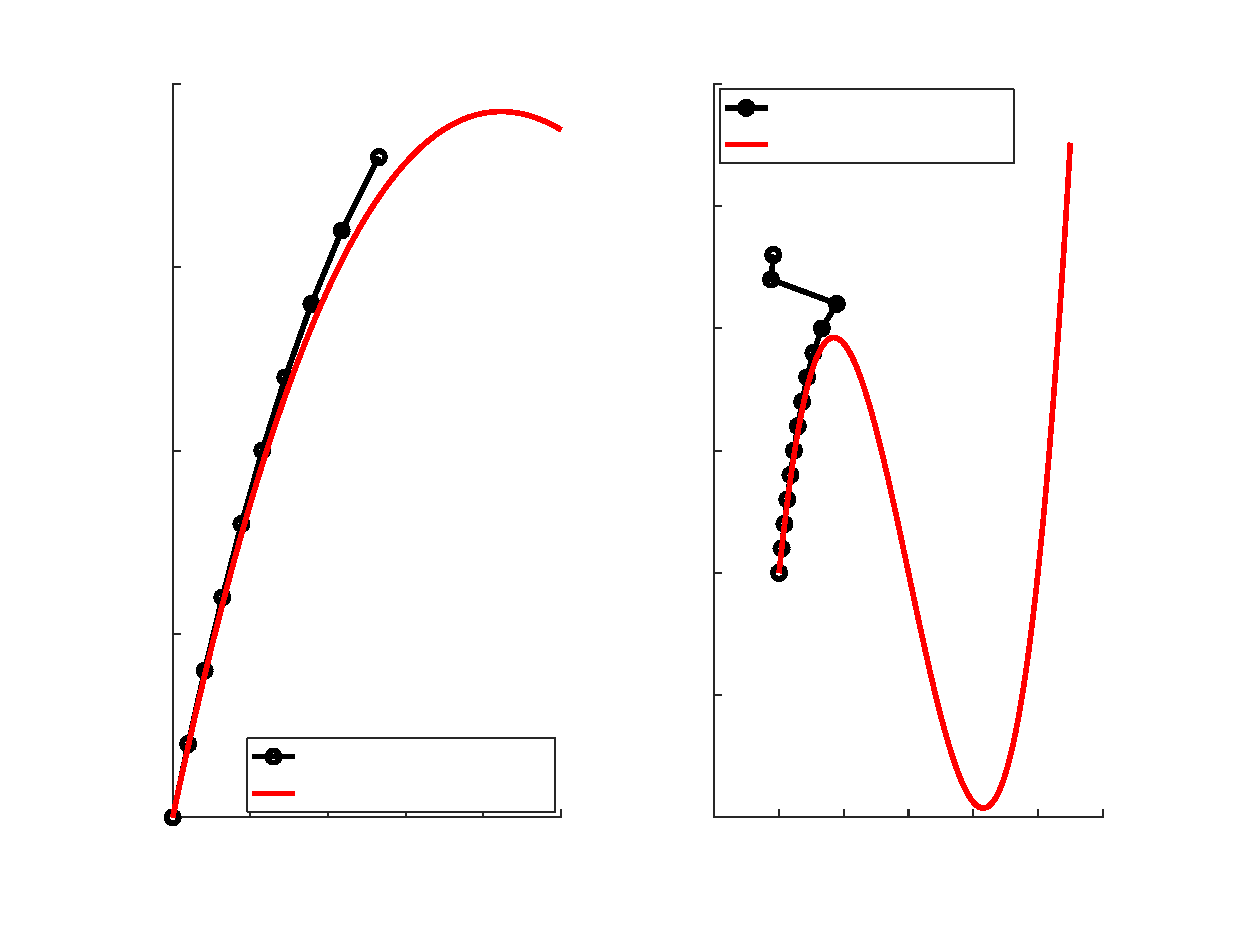
\includegraphics{Fig1Epscargabaja-inc}
\end{picture}%
\begin{picture}(576,432)(0,0)
\fontsize{15}{0}
\selectfont\put(74.88,42.5189){\makebox(0,0)[t]{\textcolor[rgb]{0.15,0.15,0.15}{{0}}}}
\fontsize{15}{0}
\selectfont\put(112.16,42.5189){\makebox(0,0)[t]{\textcolor[rgb]{0.15,0.15,0.15}{{0.1}}}}
\fontsize{15}{0}
\selectfont\put(149.44,42.5189){\makebox(0,0)[t]{\textcolor[rgb]{0.15,0.15,0.15}{{0.2}}}}
\fontsize{15}{0}
\selectfont\put(186.72,42.5189){\makebox(0,0)[t]{\textcolor[rgb]{0.15,0.15,0.15}{{0.3}}}}
\fontsize{15}{0}
\selectfont\put(224,42.5189){\makebox(0,0)[t]{\textcolor[rgb]{0.15,0.15,0.15}{{0.4}}}}
\fontsize{15}{0}
\selectfont\put(261.279,42.5189){\makebox(0,0)[t]{\textcolor[rgb]{0.15,0.15,0.15}{{0.5}}}}
\fontsize{15}{0}
\selectfont\put(69.8693,47.52){\makebox(0,0)[r]{\textcolor[rgb]{0.15,0.15,0.15}{{0}}}}
\fontsize{15}{0}
\selectfont\put(69.8693,135.54){\makebox(0,0)[r]{\textcolor[rgb]{0.15,0.15,0.15}{{0.05}}}}
\fontsize{15}{0}
\selectfont\put(69.8693,223.56){\makebox(0,0)[r]{\textcolor[rgb]{0.15,0.15,0.15}{{0.1}}}}
\fontsize{15}{0}
\selectfont\put(69.8693,311.58){\makebox(0,0)[r]{\textcolor[rgb]{0.15,0.15,0.15}{{0.15}}}}
\fontsize{15}{0}
\selectfont\put(69.8693,399.6){\makebox(0,0)[r]{\textcolor[rgb]{0.15,0.15,0.15}{{0.2}}}}
\fontsize{14}{0}
\selectfont\put(168.08,24.5188){\makebox(0,0)[t]{\textcolor[rgb]{0.15,0.15,0.15}{{$x$}}}}
\fontsize{14}{0}
\selectfont\put(30.8693,223.56){\rotatebox{90}{\makebox(0,0)[b]{\textcolor[rgb]{0.15,0.15,0.15}{{$\lambda$}}}}}
\fontsize{12}{0}
\selectfont\put(135.946,76.6871){\makebox(0,0)[l]{\textcolor[rgb]{0,0,0}{{Solución Num\'erica}}}}
\fontsize{12}{0}
\selectfont\put(135.946,59.0203){\makebox(0,0)[l]{\textcolor[rgb]{0,0,0}{{Solución Exacta}}}}
\fontsize{15}{0}
\selectfont\put(334.88,42.5189){\makebox(0,0)[t]{\textcolor[rgb]{0.15,0.15,0.15}{{-0.5}}}}
\fontsize{15}{0}
\selectfont\put(365.947,42.5189){\makebox(0,0)[t]{\textcolor[rgb]{0.15,0.15,0.15}{{0}}}}
\fontsize{15}{0}
\selectfont\put(397.014,42.5189){\makebox(0,0)[t]{\textcolor[rgb]{0.15,0.15,0.15}{{0.5}}}}
\fontsize{15}{0}
\selectfont\put(428.08,42.5189){\makebox(0,0)[t]{\textcolor[rgb]{0.15,0.15,0.15}{{1}}}}
\fontsize{15}{0}
\selectfont\put(459.147,42.5189){\makebox(0,0)[t]{\textcolor[rgb]{0.15,0.15,0.15}{{1.5}}}}
\fontsize{15}{0}
\selectfont\put(490.213,42.5189){\makebox(0,0)[t]{\textcolor[rgb]{0.15,0.15,0.15}{{2}}}}
\fontsize{15}{0}
\selectfont\put(521.28,42.5189){\makebox(0,0)[t]{\textcolor[rgb]{0.15,0.15,0.15}{{2.5}}}}
\fontsize{15}{0}
\selectfont\put(329.87,47.52){\makebox(0,0)[r]{\textcolor[rgb]{0.15,0.15,0.15}{{-0.2}}}}
\fontsize{15}{0}
\selectfont\put(329.87,106.2){\makebox(0,0)[r]{\textcolor[rgb]{0.15,0.15,0.15}{{-0.1}}}}
\fontsize{15}{0}
\selectfont\put(329.87,164.88){\makebox(0,0)[r]{\textcolor[rgb]{0.15,0.15,0.15}{{0}}}}
\fontsize{15}{0}
\selectfont\put(329.87,223.56){\makebox(0,0)[r]{\textcolor[rgb]{0.15,0.15,0.15}{{0.1}}}}
\fontsize{15}{0}
\selectfont\put(329.87,282.24){\makebox(0,0)[r]{\textcolor[rgb]{0.15,0.15,0.15}{{0.2}}}}
\fontsize{15}{0}
\selectfont\put(329.87,340.92){\makebox(0,0)[r]{\textcolor[rgb]{0.15,0.15,0.15}{{0.3}}}}
\fontsize{15}{0}
\selectfont\put(329.87,399.6){\makebox(0,0)[r]{\textcolor[rgb]{0.15,0.15,0.15}{{0.4}}}}
\fontsize{14}{0}
\selectfont\put(428.08,24.5189){\makebox(0,0)[t]{\textcolor[rgb]{0.15,0.15,0.15}{{$x$}}}}
\fontsize{14}{0}
\selectfont\put(295.87,223.56){\rotatebox{90}{\makebox(0,0)[b]{\textcolor[rgb]{0.15,0.15,0.15}{{$\lambda$}}}}}
\fontsize{12}{0}
\selectfont\put(362.882,388.1){\makebox(0,0)[l]{\textcolor[rgb]{0,0,0}{{Solución Numérica}}}}
\fontsize{12}{0}
\selectfont\put(362.882,370.433){\makebox(0,0)[l]{\textcolor[rgb]{0,0,0}{{Solución Exacta}}}}
\end{picture}
}
	%	\includegraphics[width=1\linewidth]{sourcesJBBG/Fig1}
	\caption{Soluciones obtenidas usando Euler Hacia Adelante. Izquierda: solución para $\lambda^*=0.18$. Derecha: solución para $\lambda^*=0.26$.}
	\label{fig:fig1}
\end{figure}

Los resultados obtenidos permiten establecer que el método incremental descrito tiene dificultades para resolver el sistema más allá de puntos en los cuales se cumple que: $\det(\bfF_x)=0$ ($f'=0$ en este caso). %
%
Por otra parte el efecto de \textit{drift} puede provocar que las soluciones tengan errores considerables si el incremento no es cuidadosamente seleccionado. %
%
Estas desventajas del método motivan a introducir los métodos iterativos en la siguiente sección.



\lstinputlisting[caption = {Implementación del Método de Euler para Ejemplo Numérico 1.}\label{cod:ejnonlin}]{../src/Incremental1dof.m}
%
%
\subsection{Métodos Iterativos}\label{Iter}

Luego de haber presentado los métodos incrementales y observar desventajas como el fenómeno de \textit{drift}, se plantea en esta sección la resolución del problema en cuestión por medio de métodos iterativos. %

La idea fundamental de los métodos iterativos es fijar el valor del parámetro $\lambda=\lambda_k$ y hallar el vector $\bfx_k$ que verifica la ecuación no lineal: $\bff(\bfx_k)-\lambda_k \bfv=0$. De esta manera las incógnitas del sistema no lineal son solamente las entradas del vector $\bfx_k$.

El procedimiento consiste en, dado un vector inicial $\bfx_k^{(0)}$, iterar mediante alguna regla de manera de asegurar que el vector obtenido ($\bfx_k^{(N)}$) satisface la ecuación no lineal con una tolerancia definida a priori, siendo $N$ el número de iteraciones requeridas. %
%
La expresión matemática asociada a satisfacer la ecuación no lineal es:
%
\begin{equation}\label{ec9}
	\| \bff(\bfx_k^{(N)}) - \lambda_k \bfv \| < \epsilon_{tol}.
\end{equation}

Este procedimiento iterativo suele llamarse ``iterar hasta obtener convergencia''. %
%
Iterar hasta satisfacer la condición dada por la Ecuación~\eqref{ec9} garantiza que se habrá obtenido un punto $(\lambda_k,\bfx_k^{(N)})$ para el cual se tiene un error controlado respecto de la solución exacta. Es por esto que los métodos iterativos eliminan el problema de \textit{drift}.



A continuación se presenta una de las reglas iterativas más populares para resolver sistemas de ecuaciones no lineales, el llamado Método de Newton-Raphson.

\subsubsection{Método de Newton-Raphson} \label{sec:NRcap1}

En el Método de Newton-Raphson (NR) se asume que se cuenta con un vector $\bfx_k^{(0)}$ próximo a la solución buscada $\bfx_k$ de la Ecuación~\eqref{ec2}. Para una ecuación no lineal con una sola incógnita, el método se puede deducir mediante un argumento geométrico, mientras que para un sistema de ecuaciones no lineales, la deducción requiere del concepto de linealización de funciones vectoriales.

A modo de referencia, el software SAP 2000\textsuperscript{\textregistered} \footnote{desarrollado por \textit{Computers and Structures Inc.}}, utiliza iteraciones de N-R para resolver problemas con no linealidad geométrica, permitiendo al usuario definir parámetros básicos del método.


\paragraph{Una Ecuación y Una Variable:} %
%
Se describe a continuación la deducción geométrica para el caso de una sola incógnita. De acuerdo a lo que se muestra en la Figura~\ref{fig:fig2}, la idea del método es trazar la tangente a la curva $(x,f(x))$ en el punto conocido $x_k^{(0)}$ y hallar la intersección de esta recta tangente con la recta horizontal dada por el nivel de carga definido: $\lambda_k \bfv$. %
%
El valor de $x$ en esta intersección será la nueva aproximación de la solución de la ecuación no lineal $x_k^{(1)}$.

\begin{figure}[htb]
	\centering
   \def\svgwidth{0.7\textwidth}
\input{../fig/esquemaIterNR.pdf_tex}
	\caption{Representación geométrica de iteración de Newton-Raphson.}
	\label{fig:fig2}
\end{figure}

La ecuación de recta de la tangente en el punto $x_k^{(0)}$ está dada por:
%
\begin{equation}
	\lambda v = f(x_k^{(0)})+f'(x_k^{(0)})(x-x_k^{(0)}),
\end{equation}
%
mientras que la ecuación de la recta horizontal correspondiente al nivel de carga especificado es:
%
\begin{equation}
	\lambda v = \lambda_k v.
\end{equation}

La intersección de ambas rectas provee la siguiente ecuación lineal en $x$:
%
\begin{equation}
\lambda_k v = f(x_k^{(0)})+f'(x_k^{(0)})(x-x_k^{(0)}).
\end{equation}

Resolviendo $x$ en la ecuación anterior y definiendo ese valor como la nueva aproximación de la solución: $x_k^{(1)}$,
se llega a:
%
\begin{equation}
x_k^{(1)}=x_k^{(0)}-\frac{f(x_k^{(0)})-\lambda_k v}{f'(x_k^{(0)})}.
\end{equation}

El procedimiento anterior permite definir el método iterativo de Newton-Raphson:
%
\begin{equation}\label{NR1}
\text{N-R}
	\begin{cases} 
	\displaystyle
		x_k^{(i+1)}=x_k^{(i)}-\frac{f(x_k^{(i)})-\lambda_k v}{f'(x_k^{(i)})} \\
		x_k^{(0)}
	\end{cases}
\end{equation}

Es claro a partir de la Ecuación~\eqref{NR1} que este método no puede iterar si la derivada primera de $f(x)$ es igual a cero en el punto donde se traza la tangente. Esta limitación también estará presente en el caso de Newton-Raphson para varias variables.


\paragraph{Sistema de $n$ Ecuaciones y $n$ Variables:} %
%
A continuación se presenta la deducción del método de Newton-Raphson para un sistema de $n$ ecuaciones no lineales con $n$ incógnitas. Se trabajará con el sistema de ecuaciones no lineales dado en la Ecuación~\eqref{ec3}. %
%
Para deducir el método, se linealiza el sistema de ecuaciones no lineales en el punto actual de la iteración $\bfx_k^{(i)}$. Esto se efectúa mediante un desarrollo de Taylor de $\bff$ respecto de la variable $\bfx$ en un entorno de $\bfx_{k}^{(i)}$:
%
\begin{equation}
	\lambda \bfv = \bff(\bfx_k^{(i)})+\bfF_x(\bfx_k^{(i)})(\bfx-\bfx_k^{(i)})+O(\|\bfx-\bfx_k^{(i)}\|^2)
\end{equation}

Imponiendo que $\lambda \bfv=\lambda_k \bfv$ y truncando el término de mayor orden se obtiene un sistema de ecuaciones  lineales en la variable $\bfx$:
%
\begin{equation}\label{ec10}
\lambda_k \bfv = \bff(\bfx_k^{(i)})+\bfF_x(\bfx_k^{(i)})(\bfx-\bfx_k^{(i)})
\end{equation}

Se define el paso del método de Newton-Raphson como $\Delta \bfx_k^{(i)}=\bfx_k^{(i+1)}-\bfx_k^{(i)}$ y a partir de la Ecuación~\eqref{ec10} se obtiene:
%
\begin{equation}\label{NR2}
\text{N-R}
\begin{cases} 
	\bfF_x(\bfx_k^{(i)})\Delta \bfx_k^{(i)} =-\left((\bff(\bfx_k^{(i)})-\lambda_k \bfv\right)\\
	\bfx_k^{(i+1)}=\bfx_k^{(i)}+\Delta \bfx_k^{(i)} \\
	\bfx_k^{(0)}
\end{cases}
\end{equation}

\cajaactividad{
Verificar que si $x\in\mathbb{R}$ el método dado por la Ecuación~\eqref{NR2} se reduce al presentado en la Ecuación~\eqref{NR1}.}

Asumiendo que el punto de arranque ($\bfx_k^{(0)}$) está suficientemente cerca de la solución buscada, la sucesión de iterados que genera N-R converge con orden 2. Esto significa que las distancias entre cada iterado y la solución exacta ($\bfx_k$) verifican $\|\bfx_k^{(i+1)}-\bfx_k\| \approx \beta \|\bfx_k^{(i)}-\bfx_k\|^2$, siendo $\beta>0$ la velocidad de convergencia. %
%
En este documento no se presentarán formalmente los conceptos de orden y velocidad de convergencia, ver \citep{quarteroni2007numeric} por dichas definiciones.

El método de N-R presentado en (\ref{NR2}) requiere que $\bfF_x(\bfx_k^{(i)})$ sea invertible para poder calcular el paso iterativo. Más en general, para poder tener pasos iterativos con precisión confiable se deberá cumplir que el número de condición de la matriz $\bfF_x(\bfx_k^{(i)})$ sea pequeño. Ver la Sección 7.6 del libro \citep{dahquist2008numeric} por más detalles sobre estimación de número de condición, perturbaciones y errores en sistemas lineales.

En la introducción a los métodos iterativos, en la Sección \ref{Iter}, se introdujo un criterio de parada general, el cual es válido evidentemente para la iteración de N-R. Existen otros posibles criterios de parada, como por ejemplo fijar un límite máximo para el número de iteraciones: $i\leq \text{MAXITER}$. Otro criterio puede ser iterar hasta que la diferencia relativa entre dos iterados sea menor que una tolerancia $\epsilon_{rel}$:
%
\begin{equation}
	\frac{\|\Delta \bfx_k^{(i)}\|}{\|\bfx_k^{(i+1)}\|} < \epsilon_{rel}
\end{equation}

En cada iteración de N-R se debe resolver un sistema de tamaño $(n \times n)$. Dependiendo de la estructura de la matriz $\bfF_x(x_k^{(i)})$ esta solución puede llevarse a cabo de maneras más eficientes que una escalerización de Gauss genérica. En el capítulo 8 de \citep{Bathe2014} se pueden ver en detalle métodos numéricos eficientes usados para la solución de dichos sistemas lineales.

La evaluación de la matriz $\bfF_x$ y su factorización (solución del sistema lineal) en cada paso de N-R tiene un costo elevado. Existen otros métodos numéricos iterativos que evitan evaluar $\bfF_x$ en cada iteración, o que utilizan una definición distinta para $\bfF_x$ de manera de obtener solución con menor costo computacional en cada iteración.

\subsubsection{Método de Newton-Raphson Modificado}

El método de N-R modificado presenta una alternativa para no tener que evaluar y factorizar la matriz $\bfF_x$ en cada iteración. Precisamente esto es lo que define al método en cuestión, el mismo deja fija la matriz $\bfF_x(\bfx_k^{(0)})$ a lo largo de las iteraciones.

Algunas herramientas computacionales, como por ejemplo el software SAP 2000\textsuperscript{\textregistered}, resuelven problemas con no linealidad geométrica realizando un cierto número de iteraciones de NR modificado para luego pasar a realizar iteraciones Newton-Raphson si no se alcanza convergencia.

La iteración de Newton-Raphson modificado puede ser escrita como:
%
\begin{equation}\label{NRM}
\text{N-R Modif.}
\begin{cases} 
\bfF_x(\bfx_k^{(0)})\Delta \bfx_k^{(i)} =-\left((\bff(\bfx_k^{(i)})-\lambda_k \bfv\right)\\
\bfx_k^{(i+1)}=\bfx_k^{(i)}+\Delta \bfx_k^{(i)} \\
\bfx_k^{(0)}
\end{cases}
\end{equation}

Esto permite factorizar la matriz $\bfF_x(\bfx_k^{(0)})$ al comienzo de las iteraciones y almacenar dichos factores. Luego, en cada paso iterativo se deberá resolver una sustitución hacia adelante y una sustitución hacia atrás para hallar $\Delta \bfx_k^{(i)}$. El costo computacional de dichas sustituciones es un orden de magnitud menor (en $n$) que el de la factorización de la matriz $\bfF_x(\bfx_k^{(0)})$.

Como contrapartida al costo computacional reducido de N-R Modificado, se destaca que el orden de convergencia del método es 1. Esto implica que las distancias entre cada iterado y la solución exacta ($\bfx_k$) verifican $\|\bfx_k^{(i+1)}-\bfx_k\| \approx \beta \|\bfx_k^{(i)}-\bfx_k\|$, con $\beta \in (0,1)$.

\subsubsection{Métodos Cuasi-Newton}

La familia de métodos cuasi-Newton comprende a aquellos en los cuales se cambia la matriz $\bfF_x$ del método de Newton-Raphson (matriz tangente) por una matriz más económica de evaluar y factorizar (matriz secante).

En el caso de una sola ecuación y una sola incógnita, el Método de la Secante corresponde a un método cuasi-Newton. %
%
En éste método, en lugar de trazar la tangente por el punto actual ($x_k^{(i)}$), se traza la secante por el punto actual y el anterior como se muestra en la Figura \ref{fig:fig3}.
%
\begin{figure}[htb]
	\centering
   \def\svgwidth{0.7\textwidth}
\input{../fig/esquemaIterQN.pdf_tex}
	\caption{Esquema Geométrico del Método de la Secante}
	\label{fig:fig3}
\end{figure}

Es claro que se deben especificar dos puntos de arranque para poder comenzar a iterar con el Método de la Secante.

\cajaactividad{
Verificar que la expresión de la iteración del Método de la secante está dada por:
%
\begin{equation}
	x_k^{(i+1)}=x_k^{(i)} -\frac{x_k^{(i)}-x_k^{(i-1)}}{f(x_k^{(i)})-f(x_k^{(i-1)})}\left(f(x_k^{(i)})-\lambda_k \bfv \right)
\end{equation}
}

El Método de la Secante tiene orden de convergencia super-lineal ($\text{Orden}=\frac{1+\sqrt{5}}{2}$), lo cual lo posiciona como más lento que N-R pero más rápido que N-R Modificado.

La generalización del Método de la Secante a sistemas de ecuaciones no lineales corresponde al Método de Broyden. %
%
En ese método, en lugar de la matriz tangente $\bfF_x$ utilizada en N-R, se utiliza una matriz secante que verifica una relación en los incrementos de $\bff(\bfx)$ y $\bfx$ de la forma: $\Delta \bff_k = \bfB_k \Delta \bfx_k$. La condición de matriz secante no es suficiente para definir la completamente y es ahí donde surgen distintas variantes. %
%
En la Sección 7.1.4 de \citep{quarteroni2007numeric} se presenta una definición más detallada del método. %

Otro método cuasi-Newton que deriva de la condición secante mencionada anteriormente es el Método BFGS, cuya formulación puede encontrarse en la Sección 8.4.2 de \citep{Bathe2014}.

El motivo por el cual estos métodos son atractivos es que en ellos las inversas de las matrices secantes se actualizan de forma computacionalmente económica a partir de las anteriores. Se obtiene, por lo tanto, un compromiso entre velocidad y economía computacional.

\subsubsection{Ejemplo Numérico 2: Soluciones Iterativas}

Se resuelve nuevamente la ecuación no lineal vista en el ejemplo dado en la Sección~\ref{ej1}, dada por la expresión:
%
\begin{equation}
x-\frac{3}{2}x^2+\frac{1}{2}x^3-\lambda=0
\end{equation}

En este caso se fija el nivel de carga $\lambda_k=0.19$ y se comienza la iteración desde $x_k^{(0)}=0$. %
%
La expresión del Método de Newton-Raphson para la ecuación no lineal a resolver está dada por:
%
\begin{equation}
x_k^{(i+1)}=x_k^{(i)}-\frac{x_k^{(i)}-\frac{3}{2}{x_k^{(i)}}^2+\frac{1}{2}{x_k^{(i)}}^3-0.19 }{1-3x_k^{(i)}+\frac{3}{2}{x_k^{(i)}}^2},
\end{equation}
%
mientras que la iteración del Método de Newton-Raphson Modificado está dada por:
%
\begin{equation}
x_k^{(i+1)}=x_k^{(i)}-\frac{x_k^{(i)}-\frac{3}{2}{x_k^{(i)}}^2+\frac{1}{2}{x_k^{(i)}}^3-0.19 }{1}.
\end{equation}

La implementación de ambos métodos se presenta al final de esta sección, en el Código \ref{cod:EjNum2}. %
%
En la Figura~\ref{fig:fig4} se muestran resultados obtenidos al aplicar los métodos a la resolución del ejemplo considerando $\epsilon_{tol}=10^{-8}$. %
%

\begin{figure}[htb]
	\centering
	\resizebox{\textwidth}{!}{% Title: gl2ps_renderer figure
% Creator: GL2PS 1.4.0, (C) 1999-2017 C. Geuzaine
% For: Octave
% CreationDate: Fri Dec 29 11:28:09 2017
\setlength{\unitlength}{1pt}
\begin{picture}(0,0)
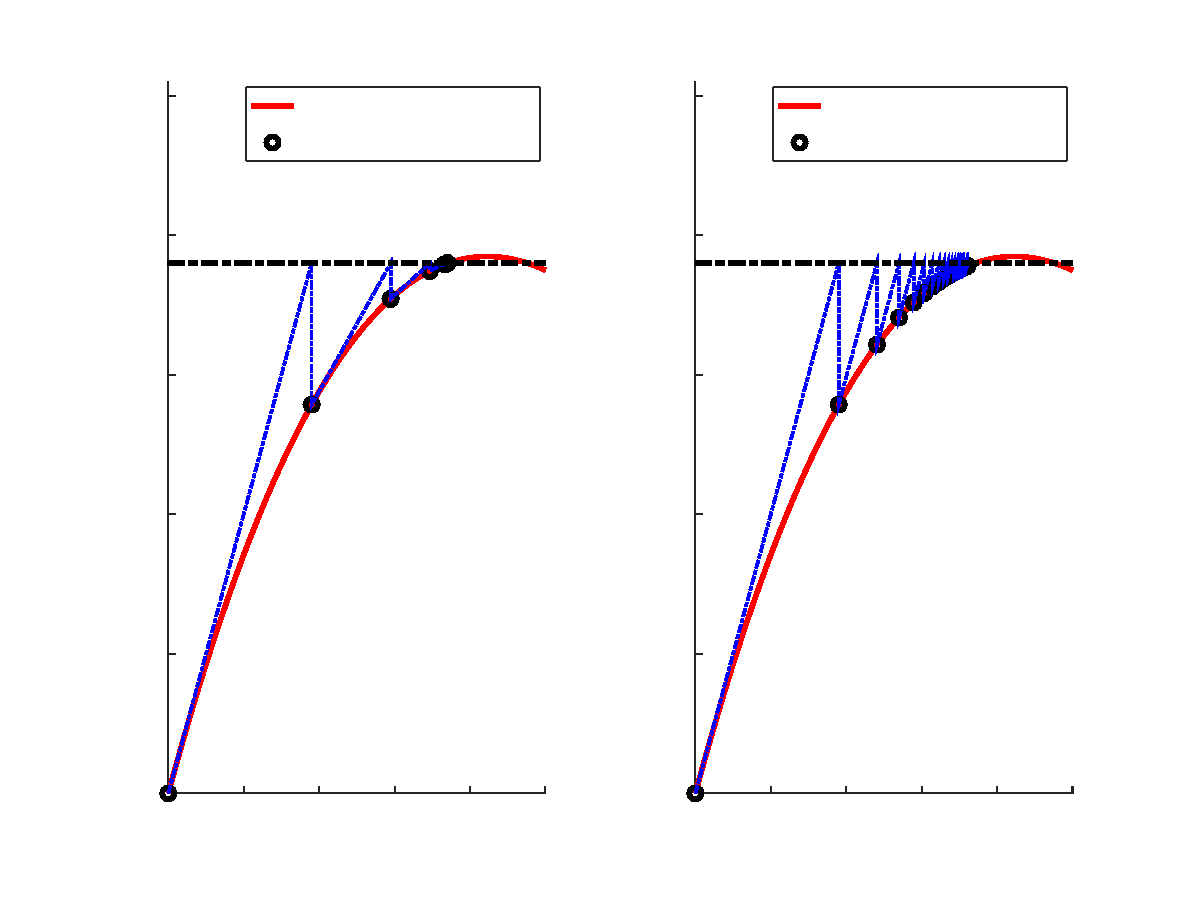
\includegraphics{Fig4Epscargabaja-inc}
\end{picture}%
\begin{picture}(560,419)(0,0)
\fontsize{15}{0}
\selectfont\put(72.8,41.0829){\makebox(0,0)[t]{\textcolor[rgb]{0.15,0.15,0.15}{{0}}}}
\fontsize{15}{0}
\selectfont\put(109,41.0829){\makebox(0,0)[t]{\textcolor[rgb]{0.15,0.15,0.15}{{0.1}}}}
\fontsize{15}{0}
\selectfont\put(145.2,41.0829){\makebox(0,0)[t]{\textcolor[rgb]{0.15,0.15,0.15}{{0.2}}}}
\fontsize{15}{0}
\selectfont\put(181.4,41.0829){\makebox(0,0)[t]{\textcolor[rgb]{0.15,0.15,0.15}{{0.3}}}}
\fontsize{15}{0}
\selectfont\put(217.6,41.0829){\makebox(0,0)[t]{\textcolor[rgb]{0.15,0.15,0.15}{{0.4}}}}
\fontsize{15}{0}
\selectfont\put(253.799,41.0829){\makebox(0,0)[t]{\textcolor[rgb]{0.15,0.15,0.15}{{0.5}}}}
\fontsize{15}{0}
\selectfont\put(67.8,46.09){\makebox(0,0)[r]{\textcolor[rgb]{0.15,0.15,0.15}{{0}}}}
\fontsize{15}{0}
\selectfont\put(67.8,113.048){\makebox(0,0)[r]{\textcolor[rgb]{0.15,0.15,0.15}{{0.05}}}}
\fontsize{15}{0}
\selectfont\put(67.8,180.006){\makebox(0,0)[r]{\textcolor[rgb]{0.15,0.15,0.15}{{0.1}}}}
\fontsize{15}{0}
\selectfont\put(67.8,246.964){\makebox(0,0)[r]{\textcolor[rgb]{0.15,0.15,0.15}{{0.15}}}}
\fontsize{15}{0}
\selectfont\put(67.8,313.921){\makebox(0,0)[r]{\textcolor[rgb]{0.15,0.15,0.15}{{0.2}}}}
\fontsize{15}{0}
\selectfont\put(67.8,380.879){\makebox(0,0)[r]{\textcolor[rgb]{0.15,0.15,0.15}{{0.25}}}}
\fontsize{14}{0}
\selectfont\put(163.3,23.0829){\makebox(0,0)[t]{\textcolor[rgb]{0.15,0.15,0.15}{{$x$}}}}
\fontsize{14}{0}
\selectfont\put(28.8,216.832){\rotatebox{90}{\makebox(0,0)[b]{\textcolor[rgb]{0.15,0.15,0.15}{{$\lambda$}}}}}
\fontsize{12}{0}
\selectfont\put(135.466,376.102){\makebox(0,0)[l]{\textcolor[rgb]{0,0,0}{{Solución Exacta}}}}
\fontsize{12}{0}
\selectfont\put(135.466,358.477){\makebox(0,0)[l]{\textcolor[rgb]{0,0,0}{{Solución Numérica}}}}
\fontsize{15}{0}
\selectfont\put(325.801,41.0829){\makebox(0,0)[t]{\textcolor[rgb]{0.15,0.15,0.15}{{0}}}}
\fontsize{15}{0}
\selectfont\put(362,41.0829){\makebox(0,0)[t]{\textcolor[rgb]{0.15,0.15,0.15}{{0.1}}}}
\fontsize{15}{0}
\selectfont\put(398.2,41.0829){\makebox(0,0)[t]{\textcolor[rgb]{0.15,0.15,0.15}{{0.2}}}}
\fontsize{15}{0}
\selectfont\put(434.4,41.0829){\makebox(0,0)[t]{\textcolor[rgb]{0.15,0.15,0.15}{{0.3}}}}
\fontsize{15}{0}
\selectfont\put(470.6,41.0829){\makebox(0,0)[t]{\textcolor[rgb]{0.15,0.15,0.15}{{0.4}}}}
\fontsize{15}{0}
\selectfont\put(506.8,41.0829){\makebox(0,0)[t]{\textcolor[rgb]{0.15,0.15,0.15}{{0.5}}}}
\fontsize{15}{0}
\selectfont\put(320.801,46.09){\makebox(0,0)[r]{\textcolor[rgb]{0.15,0.15,0.15}{{0}}}}
\fontsize{15}{0}
\selectfont\put(320.801,113.048){\makebox(0,0)[r]{\textcolor[rgb]{0.15,0.15,0.15}{{0.05}}}}
\fontsize{15}{0}
\selectfont\put(320.801,180.006){\makebox(0,0)[r]{\textcolor[rgb]{0.15,0.15,0.15}{{0.1}}}}
\fontsize{15}{0}
\selectfont\put(320.801,246.964){\makebox(0,0)[r]{\textcolor[rgb]{0.15,0.15,0.15}{{0.15}}}}
\fontsize{15}{0}
\selectfont\put(320.801,313.921){\makebox(0,0)[r]{\textcolor[rgb]{0.15,0.15,0.15}{{0.2}}}}
\fontsize{15}{0}
\selectfont\put(320.801,380.879){\makebox(0,0)[r]{\textcolor[rgb]{0.15,0.15,0.15}{{0.25}}}}
\fontsize{14}{0}
\selectfont\put(416.3,23.0829){\makebox(0,0)[t]{\textcolor[rgb]{0.15,0.15,0.15}{{$x$}}}}
\fontsize{14}{0}
\selectfont\put(281.801,216.832){\rotatebox{90}{\makebox(0,0)[b]{\textcolor[rgb]{0.15,0.15,0.15}{{$\lambda$}}}}}
\fontsize{12}{0}
\selectfont\put(388.466,376.102){\makebox(0,0)[l]{\textcolor[rgb]{0,0,0}{{Solución Exacta}}}}
\fontsize{12}{0}
\selectfont\put(388.466,358.477){\makebox(0,0)[l]{\textcolor[rgb]{0,0,0}{{Solución Numérica}}}}
\end{picture}
}
%	\includegraphics[width=.9\linewidth]{sourcesJBBG/Fig4}
	\caption{Resultados obtenidos por métodos iterativos. Izquierda: método de Newton-Raphson. Derecha: método de Newton-Raphson Modificado.}
	\label{fig:fig4}
\end{figure}

El método Newton-Raphson Modificado requiere 20 iteraciones mientras que el método Newton-Raphson requiere 7. %
%
Vale la pena remarcar que, dado que $f'(x)$ en la solución tiene un valor cercano a cero, el método requiere un número de iteraciones considerablemente elevado para converger. %
%
Esto se puede comprender mejor si se tiene en cuenta el siguiente resultado teórico: el método de N-R tiene orden de convergencia igual a 1 cuando $f'(x)$ en la raíz es igual a 0.

\cajaactividad{Modificar los parámetros de la implementación presentada y resolver el ejemplo para $\lambda_{k}=0.26$ y otros dos valores superiores a $0.2$. %
%
Analizar los resultados y comparar con los obtenidos por el método incremental.}

\lstinputlisting[caption = {Implementación de métodos iterativos para ejemplo numérico 2.}\label{cod:EjNum2}]{../src/Iterative1dof.m}


\subsection{Métodos de Longitud de Arco (Arc-Length)}\label{ArcLength}

En esta sección se presenta una variante de Método de Longitud de Arco para la resolución de sistemas de ecuaciones no lineales parametrizados del tipo dado en la Ecuación~\eqref{ec3}. %
%
Estos métodos son estudiados en matemática aplicada en el área de continuación numérica (ver notas del curso de \textit{Análisis numérico de ecuaciones no-lineales} \citep{Doedl2014Slides} y el software AUTO-07p \citep{AUTO-07p}). %
%
Por otra parte, se destaca que estos métodos fueron inicialmente desarrollados en el área de análisis estructural. %
%
Una breve reseña histórica puede encontrarse en la Sección 9.3 de \citep{crisfield1996non}. 

La ventaja fundamental de estos métodos sobre los expuestos en las secciones anteriores es que los Métodos de Longitud de Arco permiten resolver las ecuaciones no lineales en situaciones en las cuales los métodos anteriores fallan o encuentran problemas de convergencia.

Del punto de vista estructural, el interés en poder resolver el equilibrio de estructuras más allá de puntos críticos o puntos de soluciones con matriz tangente singular (más detalles en Capítulo~\ref{cap2GNA}) se justifica en que:
%
\begin{itemize}
	\item Puede ocurrir que un punto crítico solamente sea un máximo local de la curva de carga-desplazamiento.
	\item Puede ocurrir que se desee analizar un componente asilado de una estructura, para luego incorporar ese componente a una estructura completa.
	\item En general es importante saber cual es la carga de colapso de una estructura, pero además es importante saber como es su comportamiento post-colapso, si es dúctil o frágil por ejemplo.
	\item Para saber que efectivamente se alcanzó la capacidad de carga máxima de la estructura, se debe ser capaz de resolver el equilibrio más allá de dicho punto para poder verificar que en efecto es un máximo.
	\item Para poder estudiar el estado de tensiones que la estructura tiene en su carga de colapso, se debe ser capaz de converger la solución en dicho punto de carga máxima. Esto es difícil con los métodos presentados anteriormente.
	\item En la solución de problemas elásticos-perfectamente plásticos, la carga máxima de la estructura (capacidad plástica) es difícil de obtener mediante los métodos anteriores dado que la curva de carga-desplazamiento alcanza una meseta plástica en dicha carga.
\end{itemize}

Es claro a partir de lo anterior que estos métodos son esenciales para el análisis computacional del colapso de estructuras. Algunas herramientas computacionales como: ABAQUS\textsuperscript{\textregistered}, LUSAS\textsuperscript{\textregistered}, ANSYS\textsuperscript{\textregistered} o ADINA\textsuperscript{\textregistered} tienen la capacidad de llevar a cabo análisis estáticos mediante este tipo de procedimientos.

En lo que sigue se presenta una versión básica del método de Longitud de Arco, la cual no es una implementación eficiente pero tiene como ventaja la claridad en su formulación. En la Sección 9.3 de \citep{crisfield1996non} se presenta una exposición completa de estos métodos y su historia.

La idea básica de estos métodos es considerar a $\bfx\in\mathbb{R}^n$ y $\lambda\in\mathbb{R}^+$ como incógnitas. Se requiere, naturalmente, que esas incógnitas satisfagan la Ecuación~\eqref{ec3}. %
%
Sin embargo, ésta condición por sí sola no es suficiente para tener un problema determinado, ya que se puede comprobar que en ese caso se tienen $n+1$ incógnitas y $n$ ecuaciones. Por lo tanto, los métodos de Longitud de Arco imponen una restricción adicional de manera de obtener un problema determinado.

Dependiendo de cuál sea dicha restricción adicional y la implementación elegida, se obtienen los distintos métodos que forman parte de la familia de Métodos de longitud de arco. Ver en \citep{crisfield1996non} Métodos de Longitud de Arco Linealizado, Cilíndrico y Esférico. %
%
La restricción adicional está, tal como lo indica el nombre de cada método, directamente relacionada al concepto de longitud del arco de la curva carga-desplazamiento. %
%
En la Figura~\ref{fig:fig5} se presenta un esquema geométrico de la restricción de longitud de arco. %


\begin{figure}[htb]
	\centering
   \def\svgwidth{0.65\textwidth}
\input{../fig/esquemaIterAL.pdf_tex}
	\caption{Esquema geométrico del Método de Longitud de Arco.}
	\label{fig:fig5}
\end{figure}

El incremento diferencial de la coordenada de longitud de arco $s$ puede escribirse en función de los incrementos de carga y desplazamiento como:
%
\begin{equation}
	ds^2 = \dif\bfx^T\dif\bfx+\dif\lambda^2 \psi^2 \bfv^T\bfv,
\end{equation}
%
donde $\psi$ es un factor de escala de la carga con respecto a los desplazamientos. %
%
Esta relación diferencial para la longitud de arco se puede traducir a una relación en los incrementos $\Delta \bfx$ y $\Delta \lambda$:
%
\begin{equation}\label{ec11}
\Delta l^2 = \Delta \bfx^T \Delta \bfx+\Delta \lambda^2 \psi^2 \bfv^T\bfv.
\end{equation}

Observar que el parámetro $\Delta l^2$ controla la distancia a la cual el método de Longitud de Arco busca el nuevo punto solución de la ecuación no lineal.

En lo que sigue, se asume que se tiene una solución de la ecuación $\left(\bfx_{k-1},\lambda_{k-1}\right)$ y que el arco de radio $\Delta l$ está centrado en ese punto. Con lo cual: $\Delta \bfx_k = \bfx_k - \bfx_{k-1} $ y $\Delta \lambda_k = \lambda_k - \lambda_{k-1}$.

De esta manera el sistema de ecuaciones no lineales que se deberán satisfacer en el método de Longitud de Arco propuesto son:
%
\begin{equation}\label{ec12}
\begin{cases} 
\bff(\bfx_k) - \lambda_k \bfv = 0\\
\Delta \bfx_k^T \Delta \bfx_k+\Delta \lambda_k^2 \psi^2 \bfv^T\bfv - \Delta l^2 = 0 \\
\end{cases}
\end{equation}

Para obtener la expresión de la iteración del método de Longitud de Arco se debe linealizar las ecuaciones no lineales dadas en la Ecuación~\eqref{ec12} en torno al último punto iterado: 
$$\left(\bfx_{k-1}+\Delta \bfx_k^{(i)}, \lambda_{k-1}+\Delta \lambda_k^{(i)}\right)$$  respecto de las incógnitas $\Delta \bfx_k$ y $\Delta \lambda_k$.

Luego, se resuelve el sistema lineal resultante definiendo el paso iterativo del método. %
%
Notar que se expresa la linealización e iteraciones respecto de los incrementos de las variables $\bfx$ y $\lambda$.

Las ecuaciones linealizadas resultantes son:
%
%\begin{equation}\label{ec12b}
%\begin{cases} \begin{split}
%	\bff\left(\bfx_{k-1}+\Delta \bfx_k^{(i)}\right)- \left(\lambda_{k-1}+\Delta \lambda_k^{(i)}\right) \bfv +&\\
%	\bfF_x\left(\bfx_{k-1} +\Delta \bfx_k^{(i)}\right)&\delta \bfx_k^{(i)} - \delta \lambda_k^{(i)} \bfv=0
%\end{split}\\ \\
%\begin{split}
%	{\Delta \bfx_k^{(i)}}^T \Delta \bfx_k^{(i)} + {\Delta \lambda_k^{(i)}}^2 \psi^2 \bfv^T\bfv - \Delta l^2  + &\\
%	2{\Delta \bfx_k^{(i)}}^T\delta \bfx_k^{(i)} + &2\psi^2\bfv^T\bfv\Delta \lambda_k^{(i)}\delta \lambda_k^{(i)}= 0
%\end{split} \\
%\end{cases}
%\end{equation}
%
\begin{small}
\begin{eqnarray}\label{ec12b}
\bff\!\left(\bfx_{k-1}+\Delta \bfx_k^{(i)}\right)\!-\!\left(\lambda_{k-1}+\Delta \lambda_k^{(i)}\right)\!\bfv\!+\!\bfF_x\!\left(\bfx_{k-1} +\Delta \bfx_k^{(i)}\right) \delta \bfx_k^{(i)} - \delta \lambda_k^{(i)} \bfv =\!0\\
{\Delta \bfx_k^{(i)}}^T \Delta \bfx_k^{(i)} + {\Delta \lambda_k^{(i)}}^2 \psi^2 \bfv^T\bfv - \Delta l^2 +
2{\Delta \bfx_k^{(i)}}^T\delta \bfx_k^{(i)} + 2\psi^2\bfv^T\bfv\Delta \lambda_k^{(i)}\delta \lambda_k^{(i)} = 0
\end{eqnarray}
%
\end{small}
con los incrementos iterativos definidos como
\begin{equation}\label{ec13}
		\delta \bfx_k^{(i)}=\Delta \bfx_k^{(i+1)}-\Delta \bfx_k^{(i)} \qquad \text{y} \qquad
		\delta \lambda_k^{(i)}=\Delta \lambda_k^{(i+1)}-\Delta \lambda_k^{(i)}		.
\end{equation}

La versión linealizada de la Ecuación~\eqref{ec12} se traduce en el siguiente sistema lineal a ser resuelto en cada iteración del método:
%
\begin{eqnarray}\label{ec14}
\left[\begin{array}{cc}
\bfF_x\left(\bfx_{k-1} +\Delta \bfx_k^{(i)}\right) & -\bfv\\ 
2 \left(\Delta \bfx_k^{(i)}\right)^{\text{T}} &  2\psi^2\bfv^{\text{T}}\bfv\Delta \lambda_k^{(i)} 
\end{array}\right] \cdot 
\left[\begin{array}{c} 
\delta \bfx_k^{(i)} \\
\delta \lambda_k^{(i)} 
\end{array}
\right] = \\ 
\dots 
\left[\begin{array}{c}
-\left( \bff\left(\bfx_{k-1}+\Delta \bfx_k^{(i)}\right)- \left(\lambda_{k-1}+\Delta \lambda_k^{(i)}\right) \bfv \right)\\
-\left(
    {\Delta \bfx_k^{(i)}}^{\text{T}}   \Delta \bfx_k^{(i)} 
  + {\Delta \lambda_k^{(i)}}^2 \psi^2 \bfv^{\text{T}}\bfv - \Delta l^2
\right)
\end{array}\right].
\end{eqnarray}

La regla para actualizar la solución en cada iteración se desprende de la Ecuación~\eqref{ec13}:
%
\begin{equation}\label{ec15}
\begin{cases}
	\Delta \bfx_k^{(i+1)}=\Delta \bfx_k^{(i)} + \delta \bfx_k^{(i)}\\
	\Delta \lambda_k^{(i+1)}=\Delta \lambda_k^{(i)}+\delta \lambda_k^{(i)}
\end{cases}
\end{equation}

Como en cualquier método iterativo, se debe proporcionar un punto de arranque y algún criterio de parada para terminar las iteraciones. %
%
Respecto al criterio de parada, se usarán criterios iguales a los usados en Newton-Raphson (ver Sección~\ref{Iter}). %
%
Respecto al punto de inicio de la iteración, se deben definir valores $\Delta \bfx_k^{(0)}$ y $\Delta \lambda_k^{(0)}$. %
%
Una posible opción es considerarlos igual a una fracción de los incrementos dados por el método de Euler Hacia Adelante (ver la Sección~\ref{FEuler}).

Un punto adicional por comentar que surge de analizar la Figura \ref{fig:fig5}, es que el círculo que queda definido por la restricción de Longitud de Arco corta a la curva de carga-desplazamiento en dos puntos, uno avanza la solución y el otro la retrocede. Dado lo anterior, es posible que la iteración converja al punto que hace que la solución retroceda en lugar de avanzar. Una manera de controlar esto es estudiando a medida que avanza la solución numérica si se pasó un punto crítico ($\text{Det}(\bfF_x)=0$) y en ese caso estudiar la necesidad de cambiar el signo del punto de arranque dado por Euler Hacia Adelante.

Una observación final del método presentado es que la matriz del sistema lineal dado en la Ecuación~\eqref{ec14} que debe ser resuelto en cada iteración es no simétrica y eso presenta una desventaja económica en cuanto a la resolución numérica del sistema. 

En el Capítulo~\ref{cap2GNA} se describe una implementación del Método de Longitud de Arco para $n$ grados de libertad que salva estas deficiencias. El mismo permite realizar primero un paso de tipo N-R y luego determinar el incremento de Longitud de Arco a partir de la solución de una ecuación polinómica de segundo grado. Se deben utilizar criterios adicionales para decidir cuál de las dos raíces del polinomio corresponde al avance de la solución.

\subsubsection{Ejemplo Numérico 3: Solución con Método de Longitud de Arco}

Se resuelve nuevamente la ecuación no lineal vista en el ejemplo dado en la Sección~\ref{ej1}.
%
\begin{equation}
x-\frac{3}{2}x^2+\frac{1}{2}x^3-\lambda=0
\end{equation}

En este caso se fijan los parámetros del método de Longitud de Arco con los valores: radio de Arco: $\Delta l = 0.083$, factor de escala de cargas: $\psi = 1$ y pasos de Método de Longitud de Arco: $k=1,2,...,50$.

Esto resulta en la solución numérica indicada con círculos negros en la Figura~\ref{fig:fig6}.

\begin{figure}[htb]
	\centering
	\resizebox{\textwidth}{!}{% Title: gl2ps_renderer figure
% Creator: GL2PS 1.4.0, (C) 1999-2017 C. Geuzaine
% For: Octave
% CreationDate: Fri Dec 29 11:24:35 2017
\setlength{\unitlength}{1pt}
\begin{picture}(0,0)
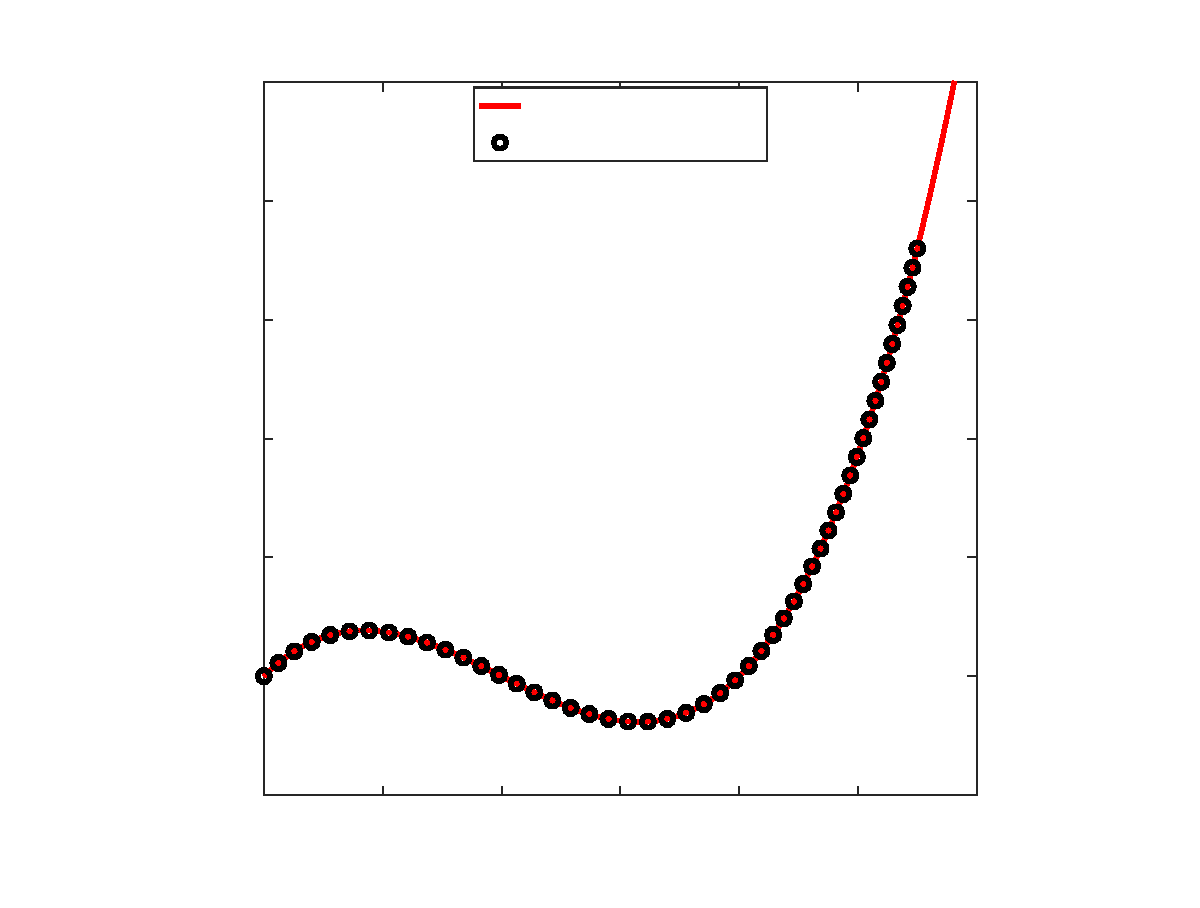
\includegraphics{Fig6Epscargabaja-inc}
\end{picture}%
\begin{picture}(560,420)(0,0)
\fontsize{15}{0}
\selectfont\put(118.65,41.1956){\makebox(0,0)[t]{\textcolor[rgb]{0.15,0.15,0.15}{{0}}}}
\fontsize{15}{0}
\selectfont\put(175.7,41.1956){\makebox(0,0)[t]{\textcolor[rgb]{0.15,0.15,0.15}{{0.5}}}}
\fontsize{15}{0}
\selectfont\put(232.75,41.1956){\makebox(0,0)[t]{\textcolor[rgb]{0.15,0.15,0.15}{{1}}}}
\fontsize{15}{0}
\selectfont\put(289.8,41.1956){\makebox(0,0)[t]{\textcolor[rgb]{0.15,0.15,0.15}{{1.5}}}}
\fontsize{15}{0}
\selectfont\put(346.85,41.1956){\makebox(0,0)[t]{\textcolor[rgb]{0.15,0.15,0.15}{{2}}}}
\fontsize{15}{0}
\selectfont\put(403.9,41.1956){\makebox(0,0)[t]{\textcolor[rgb]{0.15,0.15,0.15}{{2.5}}}}
\fontsize{15}{0}
\selectfont\put(460.95,41.1956){\makebox(0,0)[t]{\textcolor[rgb]{0.15,0.15,0.15}{{3}}}}
\fontsize{15}{0}
\selectfont\put(113.646,46.2){\makebox(0,0)[r]{\textcolor[rgb]{0.15,0.15,0.15}{{-0.5}}}}
\fontsize{15}{0}
\selectfont\put(113.646,103.25){\makebox(0,0)[r]{\textcolor[rgb]{0.15,0.15,0.15}{{0}}}}
\fontsize{15}{0}
\selectfont\put(113.646,160.3){\makebox(0,0)[r]{\textcolor[rgb]{0.15,0.15,0.15}{{0.5}}}}
\fontsize{15}{0}
\selectfont\put(113.646,217.35){\makebox(0,0)[r]{\textcolor[rgb]{0.15,0.15,0.15}{{1}}}}
\fontsize{15}{0}
\selectfont\put(113.646,274.4){\makebox(0,0)[r]{\textcolor[rgb]{0.15,0.15,0.15}{{1.5}}}}
\fontsize{15}{0}
\selectfont\put(113.646,331.45){\makebox(0,0)[r]{\textcolor[rgb]{0.15,0.15,0.15}{{2}}}}
\fontsize{15}{0}
\selectfont\put(113.646,388.5){\makebox(0,0)[r]{\textcolor[rgb]{0.15,0.15,0.15}{{2.5}}}}
\fontsize{14}{0}
\selectfont\put(289.8,23.1956){\makebox(0,0)[t]{\textcolor[rgb]{0.15,0.15,0.15}{{$x$}}}}
\fontsize{14}{0}
\selectfont\put(79.6456,217.35){\rotatebox{90}{\makebox(0,0)[b]{\textcolor[rgb]{0.15,0.15,0.15}{{$\lambda$}}}}}
\fontsize{12}{0}
\selectfont\put(244.634,377){\makebox(0,0)[l]{\textcolor[rgb]{0,0,0}{{Solución Exacta}}}}
\fontsize{12}{0}
\selectfont\put(244.634,359.333){\makebox(0,0)[l]{\textcolor[rgb]{0,0,0}{{Solución Numérica}}}}
\end{picture}
}
	\caption{Soluciones Numéricas con Método de Longitud de Arco.}
	\label{fig:fig6}
\end{figure}

Notar que el método de Longitud de Arco utilizado logra pasar por dos puntos críticos, uno en $x\simeq 0.5$ y otro en $x\simeq 1.5$.

También se puede observar en la Figura \ref{fig:fig6} que los puntos que componen la solución mediante el procedimiento de Longitud de Arco se encuentran equiespaciadas en la longitud de la curva correspondiente a la solución exacta. Se debe notar que para que dichos puntos parezcan equiespaciados, el gráfico debe tener el mismo escalado de ejes que la métrica usada como definición de longitud de arco en la Ecuación~\eqref{ec11}.

El código de Octave utilizado para generar la solución numérica se presenta en el Código~\ref{cod:EjNum3}.

\cajaactividad{
	Estudie cómo cambiar el código dado para poder resolver un sistema de ecuaciones no lineales en $\mathbb{R}^n$.}

%\bigskip

\lstinputlisting[caption = {Solución con Método de Longitud de Arco - Ejemplo Numérico 3.}\label{cod:EjNum3}]{../src/ArcLength1dof.m}







\section{Ejercicios}

%Estas l\'{\i}neas crean el entorno numerado "exercise"
\newcounter{numEjer}[section]
\newenvironment{exercise}[1][]{\addtocounter{numEjer}{1} \noindent \textbf{Ejercicio \arabic{numEjer} #1}}{}




%--------------- EJ1 ----------------------------------------------------------------------

\bigskip
\begin{exercise}
	
	En este ejercicio se usará el Método de Heun como alternativa a Euler Hacia Adelante para calcular una solución puramente Incremental.  El Método de Heun queda definido por:
	%
	\begin{equation*}
		\text{Heun}
		\begin{cases} 
			\bfp_{k+1} = \bfx_k + \Delta \lambda \cdot \bfh(\bfx_k,\lambda_k) \\
			\bfx_{k+1}= \bfx_k + \Delta \lambda \left(\bfh(\bfx_k,\lambda_k) + \bfh(\bfp_{k+1},\lambda_{k+1}) \right)/2\cdot  \\
			\bfx_0=\bfx(0)
		\end{cases}
	\end{equation*}
	
	Se pide:
	\begin{itemize}
		\item[i)] Utilizar el método de Heun para resolver el Ejemplo Numérico 1 con el mismo incremento $\Delta \lambda$ (sugerencia: utilizar el Código~\ref{cod:ejnonlin} como base para su implementación.
		%
		\item[ii)] Comparar la solución de Euler Hacia Adelante con la obtenida en el ítem anterior. Investigue cual es el orden del error cometido por Heun en cada paso y comparar contra el dado presentado para Euler Hacia Adelante.
	\end{itemize}
\end{exercise}

% ------------ EJ2 ---------------------------------------------
\bigskip
\begin{exercise}
	
	Generar mediante el Método de Newton-Raphson tres estimaciones de $\sqrt{2}$ que se expresen como fracciones de números enteros ($\sqrt{2}\simeq p/q$). Realizar el desarrollo y todos los cálculos manualmente.
	
	La primera estimación deberá utilizar enteros de un dígito, la segunda enteros de dos dígitos y la tercera de tres dígitos.
	
	Evaluar los errores absolutos de cada una de las estimaciones y verificar que la convergencia ocurre con orden 2.
	
	\smallskip
	
	\textit{Pregunta Recretiva:} \textquestiondown Existe una mejor aproximación para $\sqrt{2}$ que se exprese como el cociente de dos enteros de dos digitos que la hallada? 
	\bigskip
\end{exercise}


% ------------ EJ2 -------------------------------------------

\begin{exercise}
	
	Resolver el siguiente sistema de ecuaciones no-lineales mediante Newton-Raphson. El sistema de ecuaciones corresponde al ejemplo con dos grados de libertad de la Sección 1.3 de \citep{crisfield1996non}.
	
	$$
	\bff(x)-\lambda \bfv = 0
	$$
	%
	con $\bfx=(x_1,x_2)^T$, $\lambda \in \mathbb{R}^+$, $\bfv=(1,0)^T$
	
	$$\bff(\bfx)= \left(\begin{array}{l}
		- \frac{1}{2} x_2^2 - \epsilon x_2 + x_1 \\
		(\epsilon+x_2)\left(\frac{1}{2}x_2^2+\epsilon x_2 -x_1\right)+x_2 
	\end{array}\right)$$
	
	\bigskip
	
	Resolver para valores: $\epsilon=1/10$, $\epsilon=1/100$ y $\epsilon=1/1000$. 
	
	Dar soluciones para los valores de $\lambda=\{0;0.05;0.10;...;0.95;1.00\}$
	
\end{exercise}



\bigskip
\begin{exercise}

Las siguientes preguntas buscan que se investigue la velocidad y orden de convergencia del método de Newton-Raphson. Asuma en todos los casos que se considera ecuaciones no-lineales de la forma
	$f(x)=0$ con $f:\mathbb{R}\rightarrow \mathbb{R}$.
	\begin{itemize}
		\item[i)] Dar un ejemplo en el cual la iteración de N-R diverge de la raíz buscada.
		
		\item[ii)] Dar un ejemplo en el cual la iteración de N-R se mantiene en un bucle infinito, sin diverger ni converger a la raíz buscada.
		
		\item[iii)] ¿Puede dar un ejemplo en el cual N-R no converge a la raíz buscada con orden 2 sino con orden 1? Verificar numéricamente el orden para el ejemplo propuesto.
	\end{itemize}
	
\end{exercise}


\bigskip
\begin{exercise}
	
	En este ejercicio se plantea trabajar con un método cuasi-Newton y evaluar su orden de convergencia.
	\begin{itemize}
		\item[i)] Resolver el problema presentado en el Ejemplo Numérico 2 utilizando el Método de la Secante.
		
		\item[ii)] Evaluar numéricamente el orden de convergencia del Método de la Secante usando la iteración generada en el item anterior. Compare el valor estimado de orden de convergencia contra el valor teórico dado en las notas del curso.
		
	\end{itemize}
	
\end{exercise}

%%%%%%%%%%%%%%%%%%%%%%%%%%%%%%%%%%%%%%%%%%%%%%%%%%%%%%%%%%%%%




% ------ Capitulo 2 - Nolinealidad geometrica  ---------
%\input{sourcesJBBG/Cap2_Sec1_PMEPT} % Autor JBBG. Principio de Minima Energia Potencial Total
%\input{sourcesJBBG/Cap2_Sec2_PTV} % Autor JBBG. Principio de los Trabajos Virtuales
%\input{sourcesJBBG/Cap2_Sec3_NLSM} % Autor JBBG. Non Linear Strain Measures
%\input{sourcesJPZ/Cap2_Sec4_MEF} % Autor JPZ. Formulación de Elementos Finitos en No Linealidad Geométrica

%\input{chaps/Cap3_MNAN}

% ------ Capitulo 3 - Nolinealidad material ---------
%\chapter{No Linealidad Material}\label{cap3MNA}
%
En este capítulo se introducen herramientas básicas para el análisis de estructuras considerando no linealidad material, es decir relaciones no lineales entre tensiones y deformaciones. %
%
Se comienza presentando las ecuaciones para el análisis de estructuras de barras con relación tensión-deformación elástica no lineal, para luego pasar a introducir elementos básicos de la teoría de plasticidad.

\section{Elasticidad no lineal} \label{sec:hiper}

En esta sección se describen de forma sintética los conceptos básicos del análisis elástico considerando un comportamiento constitutivo no lineal, en particular el dado para sólidos hiperelásticos. %
%
A partir de esto se presentan las ecuaciones para estructuras de barras articuladas con comportamiento elástico no lineal. %
%
Se omitirán numerosas consideraciones teóricas importantes para el análisis de sólidos, las cuales se pueden encontrar en textos como \citep{Holzapfel2000a,Gurtin1981}.
% --------------------------------------

\subsection{Hiperelasticidad en sólidos} %
%

\subsubsection{Aspectos básicos}

Se considera un sólido que ocupa, en la configuración de referencia, la región $\Omega_0 \subset \bbR^3$, cuyo contorno es unión disjunta de $\Gamma_\bff$ y $\Gamma_\bfu$ ($\partial \Omega_0 = \Gamma_{\bfu} \cup \Gamma_{\bff}$ y $\Gamma_{\bfu} \cap \Gamma_{\bff} = \emptyset$)
, donde existe desplazamiento impuesto en $\Gamma_\bfu$ y tensiones externas $\bft_{\text{ext}}$ aplicadas en $\Gamma_\bff$. %
%
El Problema de Elasticidad no Lineal para sólidos consiste en encontrar la configuración deformada del cuerpo $\Omega_t$ de forma tal de minimizar la energía potencial total. %

Cada partícula $P$ del sólido ocupa una posición $\bfx_0$ en la configuración de referencia. %
%
En el instante de tiempo $t$ (o más formalmente para el factor de carga correspondiente a $t$) cada partícula $P$ pasa a ocupar una posición dada por el vector $\bfx_t$ el cual pertenece al conjunto de la configuración deformada $\Omega_t$. %
%
Se establece que existe una función $\chi:\Omega_0\times \bbR^+ \rightarrow \Omega_t$ que relaciona las posiciones en la configuración de referencia con las posiciones deformadas de la forma:
%
\begin{equation}
\bfx_t = \chi(\bfx_0,t).
\end{equation}
%
La función $\chi$ debe cumplir un conjunto de hipótesis relevantes que no serán consideradas en este documento, entre las que se menciona la biyectividad. %


%
Se define el campo vectorial de desplazamientos para el instante $t$, denotado como $\bfu_t:\Omega_0\rightarrow \bbR^3$, a través de la siguiente expresión:
%
\begin{equation}
\bfu_t(\bfx_0) = \bfx_t - \bfx_0.
\end{equation}
%
La dependencia de $t$ está dada de forma implícita a través del subíndice. %
%
El útil calcular el gradiente de dicho campo denotado por $\bfD$ cuya expresión se obtiene derivando ambos miembros respecto a $\bfx_0$:  
%
\begin{equation}\label{eqn:eqF}
\bfD (\bfx_0) = \bfF(\bfx_0) - \bfI,
\end{equation}
%
donde $\bfF$ es un tensor llamado gradiente de deformación dado por:
%
\begin{equation}\nonumber
\bfF(\bfx_0) = \dfrac{\partial \bfx_t}{\partial \bfx_0}(\bfx_0).
\end{equation}
%
%
Dado que se considera la deformada en un único instante, se omitió el tiempo $t$ así como también se podrá omitir la evaluación en el punto $\bfx$ de ahora en adelante. %
% -----------------------------------------------



%\subparagraph{Estado de Deformaciones .}
Sean dos puntos $\bfx_0$ y $\hat{\bfx}_0$ cercanos de la configuración de referencia y sus correspondientes puntos deformados $\bfx_t$ y $\hat{\bfx}_t$. %
%
Utilizando la definición de $\chi$ y realizando un desarrollo de primer orden respecto a $\bfx_0$ se obtiene la relación:
% 
\begin{equation} \label{eqn:relchi}
\hat{\bfx}_t - \bfx_t = \chi(\hat{\bfx}_0,t) - \chi(\bfx_0,t) \simeq \bfF(\bfx_0)(\hat{\bfx}_0-\bfx_0),
\end{equation}
%
donde se consideró que la distancia entre los puntos $\bfx_0$ y $\hat{\bfx}_0$ es pequeña. %
%
Esta identidad permite tener una relación entre los segmentos en las configuraciones de referencia y deformada.
%
La magnitud escalar $J(\bfx_0) = |\bfF(\bfx_0)|$ representa la razón de variación volumétrica local en un entorno de la partícula que ocupa la posición $\bfx_0$ en la configuración de referencia. %
%
La función de deformación $\chi$ debe cumplir ciertas hipótesis de continuidad, como por ejemplo verificar que la razón de variación volumétrica sea positiva durante todo el movimiento. %Esto está asociado a la no interpenetración del cuerpo. %
%


El estado local de deformaciones en un entorno de $\bfx_0$ está definido por lo tanto por el tensor $\bfF$, sin embargo existen diferentes definiciones de tensores que permiten representar el estado de deformaciones local. %
%
Una herramienta útil es el tensor de deformaciones de Green $\bfE$ el cual será definido de forma simplificada como una extensión de la definición considerada para elementos de barra. %
%

Se consideran los segmentos $d\bfx_0$ y $d\bfx_t$ dados por:
\begin{equation}\label{eqn:relF}
\hat{\bfx}_0 - \bfx_0 = d\bfx_0 \qquad \text{y} \qquad \hat{\bfx}_t -\bfx_t = d\bfx_t.
\end{equation}
%
Se desea aplicar la definición de la deformación de Green para calcular la expresión de la deformación unitaria del segmento $d\bfx_0$, esto es:
%
\begin{equation}
\varep_{d\bfx_0} = \frac{1}{2} \frac{d\bfx_t^{\text{T}} d\bfx_t - d\bfx_0^{\text{T}} d\bfx_0} {d\bfx_0^{\text{T}} d\bfx_0}.
\end{equation}
%
Por otra parte los segmentos $d\bfx_t$ y $d\bfx_0$ están relacionados a través de la Ecuación~\eqref{eqn:relchi} y las expresiones la Ecuación~\eqref{eqn:eqF}, por lo que se obtiene:
%
\begin{equation}
\varep_{d\bfx_0} = \frac{1}{2} d\bfx_0^{\text{T}} \left( \bfF^{\text{T}} \bfF - \bfI\right) d\bfx_0.
\end{equation}
%
Por lo que definiendo el tensor de deformaciones de Green como:
%
\begin{equation}
\bfE = \frac{1}{2} \left( \bfF^{\text{T}} \bfF - \bfI\right),
\end{equation}
%
se obtiene la siguiente expresión simplificada de la deformación unitaria:
\begin{equation}
\varep_{d\bfx_0} = d\bfx_0^{\text{T}} \bfE d\bfx_0.
\end{equation}

Se puede ver que la matriz asociada de $\bfE$ es simétrica por lo que tendrá valores propios reales. %
%
Estos valores propios representan las deformaciones unitarias de Green correspondientes a los segmentos dados por las direcciones principales. %
% ------------------------------

Sustituyendo la expresión de $\bfF$ en función del gradiente de desplazamiento dada por la Ecuación~\eqref{eqn:eqF} se obtiene
%
\begin{equation}
\bfE = \frac{1}{2} \left( \bfD + \bfD^{\text{T}} + \bfD^{\text{T}} \bfD \right).
\end{equation}
%
Se puede ver que tal como ocurre en el caso de barras, al considerar pequeñas deformaciones se obtienen equivalencias entre distintas medidas de deformación. %
%
En el caso de la medida de Green, al considerar las componentes de primer orden se obtiene:
\begin{equation}
\bfE \simeq \frac{1}{2} \left(  \bfD + \bfD^{\text{T}} \right) = \bfvarep, 
\end{equation}
%
donde $\bfvarep$ es el tensor de deformaciones infinitesimales asociado a la medida de deformación presentada en el capítulo anterior como deformación ingenieril.
% --------------------------------------------



\subsubsection{Material Hiperelástico}

Un material es elástico si y solo sí las tensiones internas producidas en el sólido dependen únicamente de la deformación actual. %
%
En el caso de un material hiperelástico, existe una función escalar, llamada densidad de energía de deformación interna, $\Psi(\bfE):\text{Sym}\rightarrow \bbR $, la cual determina el comportamiento constitutivo a través de la relación 
%
\begin{equation}
\bfS = \frac{\partial \Psi}{ \partial \bfE } (\bfE),
\end{equation}
donde $\bfS$ es el tensor de tensiones de Cosserat (o segundo tensor de Piola). %
%
Este campo tensorial está definido en puntos de la configuración de referencia y representa una de las posibles medidas de tensión a o utilizar. %
Por otra parte, el tensor de tensiones de Cauchy $\bfsig$ está definido en la configuración deformada y está relacionado con $\bfS$ a través de la expresión:
%
\begin{equation}
\bfS = J \bfF^{-1} \bfsig \bfF^{-T}.
\end{equation}
%

%
Esta función de densidad de energía de deformación permite calcular el total de energía potencial elástica $U$ acumulada por el cuerpo al ser sometido a un desplazamiento $\bfu$, a través de la expresión:
%
\begin{equation}
U(\bfu) =  \frac{1}{2} \int_{\Omega} \Psi (\bfE( \bfu ) ) \, \dif V.
\end{equation}
%
% ----------------------------------------------------


%\subparagraph{Mínima energía .} %
Tal como fue presentado en el capítulo anterior, el equilibrio está asociado a la configuración donde la energía potencial total $V$ es mínima, por lo que el problema de hallar la configuración de equilibrio consiste en un problema de optimización no lineal: %
%
%
\begin{equation}\label{eqn:prelim_minetot}
\min_{\bfu \in \mcU} \quad  U(\bfu) - \int_{\Gamma_{\bff}} \bfu^{\text{T}} \bft_{\text{ext}} \dif A,
\end{equation}
%
donde $\mcU$ es el conjunto de desplazamientos cinemáticamente admisibles, es decir compatibles con los vínculos externos. %

Al igual que en el caso de barras, las condiciones de optimalidad del problema llevan al principio de trabajos virtuales, donde las fuerzas internas están dadas por integrales en el volumen de la densidad de trabajo virtual de las tensiones internas, dadas por el producto escalar del tensor de tensiones y el tensor de deformaciones virtuales $\bfS:\delta\bfE$. %
%
Al igual que en el caso de elementos de barras existen diversos métodos numéricos que permiten resolver el problema, entre los que se encuentran algoritmos de optimización no lineal.
% ------------------------------



% --------------------------------------
\subsubsection{Funciones $\Psi$ para materiales compresibles}
%
%\subparagraph{Intro .}
Dado que el comportamiento del material es determinado por la función $\Psi$ se presentan un par de ejemplos de funciones propuestas para modelar el comportamiento constitutivo de sólidos isótropos. %
% ----------------------------

%
\paragraph{Saint-Venant Kirchoff}
El modelo de Saint-Venant-Kirchhoff establece una relación lineal entre el tensor de Cosserat y el tensor de deformaciones de Green. La expresión matemática de $\Psi$ en este caso es:
%
\begin{equation}
\Psi (\bfE) = \frac{\lambda}{2} \tra(\bfE)^2 + \mu \tra(\bfE^2),
\end{equation}
%
donde $\lambda$ y $\mu$ son dos parámetros reales del modelo que caracterizan el comportamiento del material. %
%
Esta función establece entonces una expresión para las tensiones en todo punto a partir de la deformación, dada por:
%
\begin{equation}\label{eqn:eqconssvk}
\bfS = \lambda \tra(\bfE) \bfI + 2 \mu \bfE .
\end{equation}
%
Este modelo corresponde a la ley lineal considerada en el capítulo anterior para barras con medida de deformación de Green. %
%
En el caso de pequeñas deformaciones este modelo lleva a la conocida ley constitutiva de Hooke.
% ---------------------------


\paragraph{Curnier}
%
El modelo de Saint-Venant-Kirchoff permite representar el comportamiento a tracción para grandes deformaciones aunque no es capaz de proveer buenos resultados en compresión ya que, como fue visto, se produce una pérdida de rigidez. %
%
En \citep{Curnier1994} (ver Sección 6.6.2) se describe un modelo modificado capaz de representar estados de compresión en grandes deformaciones. %
%
La expresión de la densidad de energía de deformación es:
%
\begin{equation}
\Psi (\bfE) = \lambda (J - \log(J)-1 ) + \mu \tra(\bfE^2),
\end{equation}
%
siendo el tensor de Cosserat en este caso dado por:
%
\begin{equation}
  \bfS = \lambda ( J-1 ) \bfF^{-1} \bfF^{-T}  + 2 \mu \bfE.
\end{equation}
%


\subsubsection{Funciones $\Psi$ para materiales incompresibles}
%
Existen materiales con un comportamiento constitutivo tal que se requieren elevadas cantidades de energía para poder realizar deformaciones asociadas a variaciones de volumen, es decir que las deformaciones que efectivamente desarrolla el sólido cumplen $J=1$ en todo punto. %
%
Estos materiales son llamados incompresibles y no serán considerados en este documento ya que su uso no es considerablemente frecuente en soluciones estructurales. %

Materiales como polímeros suelen ser analizados con este tipo de modelos por lo que el comportamiento de algunos elementos estructurales puede ser estudiado con este tipo de funciones $\Psi$. %
%
Existe una gran variedad de funciones de energía utilizadas en diversas aplicaciones, como por ejemplo: el modelo \textit{Neo-Hookean} uno de los más simples (ver \citep{Holzapfel2000a}), el modelo presentado por \cite{Delfino1997} apropiado para el modelado de ciertos comportamientos observados experimentalmente en arterias carótidas o el modelo de \cite{Veronda1970} el cual fue aplicado para el desarrollo de una técnica de diagnóstico de tumores malignos en mamas \citep{Goenezen2012}.


\subsubsection{Pequeñas deformaciones}

En el caso de pequeñas deformaciones se tiene que el tensor $\bfE$ es aproximadamente igual a $\bfvarep$ y que el tensor de tensiones $\bfS$ es aproximadamente igual al tensor de tensiones de Cauchy $\bfsig$ en coordenadas locales (sistema co-rotacional) por lo que la definición de material hiperelástico puede ser considerada ahora como:
%
\begin{equation}
  \bfsig = \frac{\partial \psi}{\partial \bfvarep} (\bfvarep).
\end{equation}
%
No serán abordadas en este documento las condiciones que debe cumplir la función $\psi$, sin embargo se considerará que deberán ser funciones que garanticen al menos continuidad de la función $\bfsig(\bfvarep)$. %
%
Esta función determina la nolinealidad material para comportamiento elástico en pequeñas deformaciones.


En el caso del material de Saint-Venant-Kirchhoff para pequeñas deformaciones se obtiene una expresión de $\psi$ dada por:
%
\begin{equation}
\psi(\bfvarep) = \frac{\lambda}{2} \left( \text{Tr}(\bfvarep)\right)^2 +  \mu \left(\text{Tr}(\bfvarep^2)\right)
\end{equation}
%
y la relación del tensor de tensiones está dada por:
%
\begin{equation}
\bfsig = \frac{\partial \psi}{\partial \bfvarep} (\bfvarep) = \lambda \text{Tr}(\bfvarep) +  2 \mu \bfvarep,
\end{equation}
lo que coincide con la ecuación constitutiva del material elástico-lineal. %
%


\subsection{Hiperelasticidad en barras}

En el caso de barras con comportamiento hiperelástico el estado tensional corresponde a un estado uniaxial de tensiones. %
%
En \citep{Castrillo2014} se presenta la resolución de diversos ejemplos de reticulados tridimensionales con comportamiento hiperelástico para el material de Saint-Venant-Kichhoff deduciendo las soluciones a partir de las ecuaciones válidas para sólidos. %
%

Si un eje del sistema de coordenadas coincide con el eje de la barra entonces la componente asociada a dicha dirección será la única entrada no nula dada por
%
\begin{equation}
\sigma_x = \frac{\partial \psi}{\varepsilon_x}(\varepsilon_x) = \sigma (\varepsilon_x),
\end{equation}
%
por simplicidad se considerará que la tensión está dada por la función $\sigma(\varepsilon)$. %



% -------------------------
En el capítulo anterior se presentaron las ecuaciones del PTV, cuya aplicación lleva al sistema de ecuaciones no lineales:
%
\begin{equation}
  \bff_{\text{int}}(\bfu) - \bff_{\text{ext}} = \bszer.
\end{equation}
% ------------------
%
Para el desarrollo de los métodos numéricos la resolución de estas ecuaciones se asumió una relación constitutiva lineal. %
%
Si se continúa el desarrollo desde la Ecuación~\eqref{eqn:fueinterna} y considerando ahora una relación general no lineal entre tensión y deformación, se tiene:
%
\begin{equation}
\frac{\partial \bff^e_{\text{int}} } {\partial \bfu^e} (\bfu^{(k)}) 
= A_0^e \ell_0^e \left( \frac{\partial \bfb^e}{\partial \bfu^e} (\bfu^{(k)}) \right)^{\text{T}} \sigma^e(\varep((\bfu^{(k)})))
+ A_0^e \ell_0^e  (\bfb^e(\bfu^{(k)}))^{\text{T}} \frac{ \partial \sigma^e}{\partial \bfu^e}( \varep( \bfu^{(k)}) ).
\end{equation}

Usando la función del comportamiento no lineal y la regla de la cadena se tiene:
\begin{equation}
\frac{ \partial \sigma}{\partial \bfu}(\bfu) = E^{\text{tan}}(\varep(\bfu)) \frac{ \partial \varep}{\partial \bfu}(\bfu)
\end{equation}
donde $E^{\text{tan}}$ es el llamado módulo tangente, dado por:
\begin{equation}
E^{\text{tan}}(\varep) = \frac{ \partial \sigma}{\partial \varep} (\varepsilon).
\end{equation}

Sustituyendo en la ecuación de la derivada de las fuerzas internas se tiene:
\begin{equation}
\frac{\partial \bff_{\text{int}}^e } {\partial \bfu^e} (\bfu^{(k)})
= \frac{\sigma ( \varep( \bfu^{(k)}) ) A_0 }{\ell_0} \bfG^e
+  (\bfb^e(\bfu^{(k)}))^{\text{T}} \,  E^{\text{tan}} (\varepsilon(\bfu^{(k)})) A_0^e \ell_0^e \, \bfb^e(\bfu^{(k)}).
\end{equation}

El proceso de ensamblado de la matriz tangente y resolución del método Newton-Raphson es similar al realizado para análisis con nolinealidad geométrica, teniendo en cuenta que el vector de fuerzas internas debe ser calculado con la tensión dada por la relación no lineal.


La herramienta ONSAS permite que el usuario introduzca cualquier modelo hiperelástico para el comportamiento de las barras a través de la función \textit{hyperElasModels}.


\subsection{Análisis de reticulados bi-modulares}



%\subsection{Condiciones de optimalidad KKT}
%
%
%\begin{equation}
%\left\{
%\begin{array}{l}
%\min_{x} \qquad  f(x)\\
%\text{s.a.}\\
%\quad g(x)\leq 0\\
%\quad h(x) = 0
%\end{array}
%\right.
%\end{equation}
%
%
%
%\begin{equation}
%\left\{
%\begin{array}{l}
%\nabla f(x) + \lambda \nabla g(x) + \mu \nabla h(x) = 0\\
%g(x)\leq 0\\
%h(x) = 0\\
%\lambda \geq 0\\
%\lambda g(x) = 0
%\end{array}
%\right.
%\end{equation}


Existe un grupo importante de materiales llamados bi-modulares (en ingles \textit{bi-modulus materials}), los cuales se caracterizan por tener diferente comportamiento constitutivo a tracción y a compresión. %
%
Entre algunos ejemplos se encuentran la madera y el hormigón, cuyo análisis simplificado es generalmente realizado sin tomar en cuenta esta no linealidad. %
%

Por otra parte en elementos estructurales como cables o tensores se puede considerar que el elemento no soporta esfuerzos de compresión, lo que puede modelarse como un comportamiento constitutivo no lineal para desplazamientos pequeños.
% 

\subsubsection{Abordaje mediante PTV y métodos iterativos}

El abordaje asociado al PTV y los correspondientes métodos iterativos pueden ser aplicados considerando la función $\sigma$ y su derivada en las ecuaciones de PTV y los correspondientes métodos numéricos. Estas expresiones son: %
%
\begin{equation}
\sigma (\varepsilon) = 
\left\{
\begin{array}{lr}
E_T \varepsilon & \text{si } \varep \geq 0 \\
E_C \varepsilon & \text{si }\varep <0
\end{array}
\right.
\qquad
\frac{\partial \sigma}{\partial \varep} (\varepsilon) = 
\left\{
\begin{array}{lr}
E_T & \text{si }\varep \geq 0 \\
E_C & \text{si }\varep < 0
\end{array}
\right.
\end{equation}
%
donde $E_C$ y $E_T$ son los módulos de Young a compresión y tracción respectivamente.
%
Un caso de particular interés es el del análisis de tensores en el cual se puede considerar $E_C=0$.

\cajaactividad{Modificar el Código~\ref{cod:cerchamises} para resolver el problema de la cercha de Von Mises considerando un comportamiento bi-modular para ambas barras donde la rigidez a compresión es la mitad de la rigidez a tracción. Validar los resultados del código comparando con soluciones analíticas para pequeños desplazamientos.}


\subsubsection{Formulaciones alternativas}

Los métodos iterativos son eficientes y permiten garantizar convergencia considerando como hipótesis fundamental que la función de fuerzas residuales $\bfr$ tiene derivadas continuas. %
%
Para este tipo de materiales esto no se cumple, por lo que los resultados de convergencia obtenidos para este tipo de estructuras podrían ser de menor calidad, provocando que para alguna estructura no sea posible obtener convergencia.

Existen otros enfoques basados en formulaciones de optimización y programación cuadrática que permiten resolver este tipo de problemas aplicando algoritmos eficientes logrando mejores resultados en términos de convergencia. %
%
En \citep{Zhang2013} se presenta una de estas formulaciones alternativas mostrando a través de la resolución de algunos ejemplos que, según los autores, el método de NR no logra converger a la solución para ciertos criterios de parada establecidos. %
%
En \citep{Zhang2016a} se presenta también una extensión de este enfoque para problemas de sólidos, mientras que en \citep{Du2014} se presenta una de las primeras formulaciones teóricas basadas en enfoques energéticos.


% ===========================================================================
% ===========================================================================
\section{Introducción a la Teoría de Plasticidad}

En esta sección se presenta una introducción a la Teoría de Plasticidad para cuerpos sometidos a pequeñas deformaciones. %
%
La presentación es realizada a través de la descripción de las ecuaciones de la teoría de plasticidad unidimensional, suficiente para introducir todos los conceptos de la misma, dentro del objetivo de este documento.

Existen textos que presentan diversos enfoques a esta teoría, entre los que se destaca por una parte \citep{Jirasek2001} con un abordaje teórico orientado a aplicaciones estructurales, y por otra parte \citep{DeSouzaNeto2008,Taroco2017,Simo1998} con enfoques teóricos generales de mecánica del continuo aplicables al análisis de sólidos sometidos a diversas acciones externas. %
%
Se recomienda complementar los conceptos presentados en esta sección con alguno de los libros mencionados.

\subsection{Teoría unidimensional de plasticidad}

Se considera una barra sometida a una historia de deformaciones tal que parte de la deformación axial es remanente, es decir que se mantendrá luego de retirar las cargas externas. %
%
Esta deformación remanente es producida cuando la magnitud de la tensión alcanza un cierto valor de tensión de fluencia $\sigma_Y$.

\subsubsection{Descomposición aditiva de deformación y ley elástica}
Bajo la hipótesis de pequeñas deformaciones, es posible descomponer de forma aditiva la deformación total $\varepsilon$ en dos componentes: deformación elástica $\varepsilon^e$ y deformación \textit{plástica} o remanente $\varepsilon^p$, por lo tanto:
%
\begin{equation}
\varepsilon = \varepsilon^e + \varepsilon^p.
\end{equation}
%

Por otra parte se considera la ley elástica que establece que la relación entre la tensión y la deformación elástica es lineal y dada por:
%
\begin{equation}\label{eqn:plasleyelas}
\sigma =  E \varepsilon^e = E(\varepsilon - \varepsilon^p ),
\end{equation}
%
donde $E$ es el módulo de Young. Esta ley se cumple durante todo el proceso de deformación para cualquier valor de deformación plástica.

Es importante destacar que la deformación plástica $\varep^p$ puede ser positiva o negativa, es decir estar asociada a una extensión o un acortamiento.

\subsubsection{Función de fluencia}

El proceso de plastificación se produce cuando la tensión alcanza un valor límite o de fluencia, lo que es escrito en términos de una función llamada \textit{función de fluencia} $\Phi$. En esta sección se considerará, como ejemplo, una función dada por:
%
\begin{equation}\label{eqn:defphi}
\Phi (\sigma, \sigma_Y) = |\sigma| - \sigma_Y.
\end{equation}
%
Observe que el valor absoluto de $\sigma$ establece un comportamiento idéntico para compresiones y tracciones, esto define que el proceso de fluencia o endurecimiento sea isótropo. %
%
En modelos de mayor complejidad, y para materiales utilizados en ingeniería civil como hormigón, es usual considerar funciones que consideren de diferente forma las tensiones a compresión y tracción (ver un ejemplo en el Capítulo 1 de \citep{Simo1998}).


El comportamiento del material es elástico si se verifica:
%
\begin{equation}
\Phi(\sigma,\sigma_Y) < 0,
\end{equation}
%
donde $\sigma_Y$ es un parámetro del modelo que puede variar en el proceso de plastificación. %
%
La función $\Phi$ y el valor $\sigma_Y$ establecen por lo tanto el rango de valores de tensión $\sigma$ para los cuales el comportamiento es elástico.

En el caso de plastificación de sólidos la función $\Phi$ depende del tensor de tensiones y puede adquirir diversas formas, entre las que se destacan la función asociada el criterio de fluencia de Von Mises. %
%


Si la tensión es tal que la función de fluencia pasa a valer cero comienza un proceso de plastificación. %
%
En dicho proceso se deberá obtener un nuevo valor de $\sigma$ y eventualmente de $\sigma_Y$ tal que se continúe verificando que $\Phi(\sigma,\sigma_Y)\leq 0$. %
%
Para establecer cuáles son estos valores se utiliza el principio de máxima disipación plástica.



\subsubsection{Principio de máxima disipación plástica}

El principio de máxima disipación plástica (o máximo trabajo plástico) establece que de todas las posibles tensiones $\sigma$ que cumplen $\Phi (\sigma, \sigma_Y)\leq 0$, la tensión real producida será aquella que maximice la disipación plástica por unidad de volumen dada por $\sigma \dot{\varepsilon}$. %
%
Se puede remarcar que este último producto puede considerarse como una disipación de energía o también como una potencia de fuerzas internas, de cualquiera de las dos formas se produce una variación de energía total del sistema. 


El enunciado del principio puede plantearse como un problema de maximización como:
%
\begin{equation}
(\text{MDP})\left\{
\begin{array}{l}
\max_\sigma \quad \sigma \dot{\varepsilon}^p\\
\text{s.a.}\\
\quad \Phi(\sigma) \leq 0\\
\end{array}
\right.
\end{equation}

Para encontrar las condiciones que deben cumplir las tensiones solución del problema se plantean las condiciones de optimalidad de Karush-Kuhn-Tucker (KKT). %
%
A continuación se presentan de forma esquemática las ecuaciones de KKT (ver \citep{Luenberger2008} por detalles del desarrollo). %

\paragraph{Condiciones de Karush-Kuhn-Tucker}
Sean funciones $f(\bfx):\bbR^n \rightarrow \bbR$ y $g(\bfx):\bbR^n \rightarrow \bbR$ funciones suaves, y un problema de optimizacion no lineal dado por 
\begin{equation}
\left\{
\begin{array}{l}
\max_\bfx \quad f(\bfx)\\
\text{s.a.}\\
\quad g(\bfx) \leq 0\\
\end{array}
\right.
\end{equation}
%
todo punto $\bfx$ que satisface las condiciones de optimalidad de primer orden (''punto crítico'') debe necesariamente cumplir
%
\begin{eqnarray}
\nabla f(\bfx) &=& \eta \nabla g (\bfx)\\
g(\bfx) &\leq & 0 \\
\eta &\geq& 0\\
\eta \, g(\bfx) &=& 0,
\end{eqnarray}
donde $\eta$ es un escalar llamado multiplicador de Lagrange, a ser determinado. %
%
Estas condiciones representan un sistema de ecuaciones no lineales. %


Escribiendo las condiciones de optimalidad para el problema MDP se obtiene que la tensión debe necesariamente cumplir:
%
\begin{eqnarray}
\dot{ \varepsilon}^p &=& \eta \frac{\partial \Phi}{\partial \sigma}(\sigma,\sigma_Y) \label{eqn:condflujo}\\
\Phi(\sigma,\sigma_Y) &\leq & 0 \\
\eta &\geq& 0 \\
\eta \, \Phi(\sigma,\sigma_Y) &=& 0.
\end{eqnarray}
%
Estas condiciones permiten derivar las siguientes leyes sobre el proceso de plastificación.

\subsubsection{Ley de flujo plástico y condiciones de carga/descarga}

La condición dada por la Ecuación~\eqref{eqn:condflujo} es llamada \textit{ley de flujo plástico}. %
%
Calculando la derivada e introduciendo la variable $\gamma$ dada por $\dot{ \gamma} = \eta$ se tiene:
%
\begin{equation}\label{eqn:dotepsgam}
\dot{ \varepsilon}^p = \dot{ \gamma} \, \text{signo}(\sigma),
\end{equation}
donde se puede observar que si la tensión es de compresión, la deformación plástica decrece. %
%
Más adelante se presentará una interpretación física de la variable $\gamma$. %


Esto permite reescribir las condiciones adicionales del KKT obteniendo las llamadas condiciones de carga/descarga, dadas por:
%
\begin{eqnarray}
\dot{\gamma} &\geq& 0 \\
\Phi(\sigma,\sigma_Y) &\leq & 0\\
\dot{\gamma} \Phi(\sigma,\sigma_Y) &=& 0
\end{eqnarray}


\subsubsection{Función de endurecimiento}

La magnitud $\sigma_Y$ representa un parámetro constitutivo dado por la micro-estructura del cuerpo y otros parámetros asociados al correspondiente proceso de plastificación del material. %
%
En este modelo se considera que este valor depende de la deformación plástica acumulada a través de una función llamada \textit{función de endurecimiento}:
%
\begin{equation}
\sigma_Y = \sigma_Y (\bar{\varepsilon^p}),
\end{equation}
%
donde $\bar{\varepsilon^p}$ es la deformación plástica acumulada durante todo el proceso, es decir
%
\begin{equation}\label{eqn:epspl}
\bar{\varepsilon^p} (t) = \int_{0}^{t} |\dot{\varepsilon^p}(\tau)| \dif \tau.
\end{equation}
Esta nueva magnitud representa la \textit{memoria} del material, siendo este el elemento conceptual más relavante que define al material como no elástico.


Derivando respecto al tiempo ambos miembros de la Ecuación~\eqref{eqn:epspl} y utilizando la Ecuación~\eqref{eqn:dotepsgam} se obtiene:
%
\begin{equation}
\dot{ \bar{\varepsilon^p}} = %
|\dot{ \varepsilon^p}| = |\dot{ \gamma} \text{signo}(\sigma)| = |\dot{ \gamma} |.
\end{equation}
%
Usando que $\dot{ \gamma} \geq 0$ se tiene
%
\begin{equation}
\dot{ \bar{\varepsilon^p}}  = \dot{\gamma},
\end{equation}
%
por lo que la derivada de $\gamma$ establece la variación de la deformación plástica acumulada. %
%
Si $\gamma$ es considerada nula al inicio del proceso puede ser fácilmente interpretada como la deformación plástica acumulada, lo cual también es compatible con la condición dada por KKT de $\dot{\gamma}\geq0$, es decir que la magnitud de la deformación plástica acumulada es creciente durante todo el proceso. %
% --------------------



\subsubsection{Módulo elastoplástico tangente}

Durante un proceso de incremento de carga en el que ocurre plastificación el valor la función de fluencia debe mantenerse nulo en los instantes de tiempo inmediatamente posteriores, es decir que se verifican las condiciones:
%
\begin{equation}
\Phi = 0 \qquad \text{y} \qquad \dot{ \Phi} = 0.
\end{equation}

Derivando respecto al tiempo ambos miembros de la Ecuación~\eqref{eqn:defphi} se obtiene:
\begin{equation}
\dot{ \Phi} = \text{signo} (\sigma ) \dot{ \sigma} - \frac{\partial \sigma_Y}{\partial \bar{ \varep^p} } \dot{ \bar{ \varep^p}},
\end{equation}
%
por lo tanto, igualando a cero se tiene que durante la plastificación se cumple:
%
\begin{equation}\label{eqn:plaseq}
 \text{signo} (\sigma ) \dot{ \sigma} = \frac{\partial \sigma_Y}{\partial \bar{ \varep^p} } \dot{ \bar{ \varep^p}}.
\end{equation}
%
Multiplicando ambos miembros por $\text{signo}(\sigma)$, recordando que $\dot{ \bar{ \varep^p}} = \dot{ \gamma}$ y usando la Ecuación~\eqref{eqn:dotepsgam} se obtiene:
\begin{equation}\label{eqn:plasnueva}
\dot{ \sigma} = \frac{\partial \sigma_Y}{\partial \bar{ \varep^p} } \dot{ \varep^p}.
\end{equation}

Por otra parte, derivando la ley elástica dada por la Ecuación~\eqref{eqn:plasleyelas} se tiene la relación:
%
\begin{equation}\label{eqn:sigmdot}
  \dot{ \sigma} = E \left( \dot{ \varep} -  \dot{ \varep^p} \right).
\end{equation}
%

Despejando $\dot{ \varepsilon^p}$ de la Ecuación~\eqref{eqn:plasnueva}, sustituyendo en la Ecuación~\eqref{eqn:sigmdot} y agrupando se tiene:
%
\begin{equation}
\dot{ \sigma} = E^{\text{tan}} \dot{ \varep}
\end{equation}
%
donde $E^{\text{tan}}$ es el módulo tangente elastoplástico, dado por
%
\begin{equation} \label{eqn:Etan}
E^{\text{tan}} (\bar{ \varep^p}) = \frac{E \dfrac{\partial \sigma_Y}{\partial \bar{ \varep^p} } (\bar{ \varep^p}) }{E + \dfrac{\partial \sigma_Y}{\partial \bar{ \varep^p}  } (\bar{ \varep^p}) }.
\end{equation}
%
A partir de esta relación se puede también obtener una expresión para la pendiente de la función de endurecimiento en función de $E^{\text{tan}}$. %
%
Es importante resaltar que existe una relación implícita entre la deformación total y la deformación plástica acumulada cuyo análisis no debe ser despreciado.


La mayoría de los materiales utilizados en Ingeniería Civil suelen ser caraterizados a partir de valores de tensión y deformación (total) medidos a través de ensayos experimentales. %
%
Esto permite determinar el módulo tangente, el cual debe ser vinculado a algún modelo de elastoplasticidad a través de la función de endurecimiento para poder contar con un modelo teórico completo del comportamiento elastoplástico. %
%
En \citep{PerezZerpa2017} se presenta el desarrollo de un método para identificación de propiedades elastoplásticas y su aplicación a la caracterización mecánica de madera a partir de valores de tensión y deformación obtenidos mediante ensayos experimentales.


\subsection{Método numérico de análisis elastoplástico}

\subsubsection{Relaciones algebraicas}

Para obtener un método numérico para resolver las ecuaciones que gobiernan el proceso de plastificación, es necesario utilizar alguna regla para integrar las ecuaciones diferenciales del modelo. %

En esta sección se presenta el desarrollo de un método numérico para resolver las ecuaciones correspondientes a una barra sometida a una deformación axial, asumiendo que en cada paso se conoce la deformación total aplicada. %
%
Se considera que el rango temporal del proceso estudiado es discretizado en intervalos uniformes. Por simplicidad y sin pérdida de generalidad, se considera $\Delta t=1 $. %
%
Nuevamente, el tiempo no representa que las cargas sean aplicadas dinámicamente, sino simplemente una referencia a factores de carga o deformación impuesta.

Sea un instante de tiempo $n$ para el cual se conocen los valores de $\sigma_n$, $\varep_n$, $\bar{ \varep^p}_n$ y $\gamma_n$. %
%
Se aplica un incremento en la deformación total por lo que se conoce el valor de deformación en el instante de tiempo siguiente $\varep_{n+1} = \varep_n  + \Delta \varep$. %
%
Se desea determinar las otras magnitudes. Se comienza operando con la derivada de la ley elástica, dada por la Ecuación~\eqref{eqn:sigmdot}, donde se sustituye la Ley de flujo plástico dada por la Ecuación~\eqref{eqn:dotepsgam}. %
%
Se obtiene por lo tanto:
%
\begin{equation}
\dot{ \sigma} = E \left( \dot{ \varepsilon} - \dot{\gamma} \text{signo}(\sigma) \right).
\end{equation}
%
Se puede considerar una regla de integración de tipo Euler hacia atras o \textit{Backward Euler}, donde se integra  en el tiempo numéricamente, evaluando el integrando en el instante $n+1$, obteniendo:
%
\begin{equation}
\sigma_{n+1}  =  \sigma_n + E \Delta \varepsilon - \Delta \gamma \text{signo}(\sigma_{n+1} ).
\end{equation}

Resulta conveniente definir la magnitud $\sigma_{E,n+1}$ dada por:
%
\begin{equation}
\sigma_{E,n+1} = \sigma_n + E \Delta \varep,
\end{equation}
%
la cual representa la tensión que se obtendría si no se produce aumento de la deformación plástica para el incremento de deformación total aplicado. Esto equivale a que el incremento de tensión sea puramente elástico. %

\cajaactividad{
Mostrar que se verifica la siguiente igualdad
$$
\sigma_{E,n+1} = E(\varepsilon_{n+1} - \varepsilon^p_{n} ).
$$
}

Usando esta nueva definición se obtiene la expresión:
%
\begin{equation}\label{eqn:signp1}
\sigma_{n+1} = \sigma_{E,n+1} - E  \Delta \gamma \, \text{signo} (\sigma_{n+1}).
\end{equation}

Por otra parte se sabe que si $\Delta \gamma >0$ entonces se produce plastificación y la función $\Phi$ debe continuar siendo nula en el instante $n+1$,
por lo tanto se deberá cumplir
\begin{equation}
\Phi(\sigma_{n+1},\sigma_Y(\bar{ \varep^p}_{n+1} ) )  = |\sigma_{n+1}|- \sigma_Y ( \bar{ \varep^p}_{n+1} ) = 0 .
\end{equation}
%
Recordando la relación entre deformación plástica acumulada y $\gamma$ se tiene
\begin{equation}
|\sigma_{n+1}|- \sigma_Y ( \bar{ \varep^p}_{n} + \Delta \gamma ) = 0 .
\end{equation}

Esta relación, junto con la Ecuación~\eqref{eqn:signp1}  forman un sistema de ecuaciones no lineales, a resolver para encontrar la tensión y $\gamma$ en el instante $n+1$, dado por:
%
\begin{eqnarray}
\sigma_{n+1} &= & \sigma_{E,n+1} - E  \Delta \gamma \, \text{signo} (\sigma_{n+1}), \\
|\sigma_{n+1}| &=& \sigma_Y ( \bar{ \varep^p}_{n} + \Delta \gamma ) \label{eqn:phisigm}.
\end{eqnarray}

Para poder obtener una expresión del valor absoluto de la tensión se continúa desarrollando la identidad de la Ecuación~\eqref{eqn:signp1},
%
\begin{equation}
|\sigma_{n+1}|\text{signo}(\sigma_{n+1}) = |\sigma_{E,n+1}|\text{signo}(\sigma_{E,n+1}) - E  \Delta \gamma \, \text{signo} (\sigma_{n+1})
\end{equation}
por lo tanto se tiene:
\begin{equation}
\text{signo}(\sigma_{n+1}) \left(  |\sigma_{n+1}| + \Delta \gamma E \right) = |\sigma_{E,n+1}|\text{signo}(\sigma_{E,n+1}).
\end{equation}
%
Dado que $\Delta \gamma \geq 0$, los resultados de la función signo de cada miembro son multiplicados por valores no negativos por lo tanto deben tener el mismo resultado, obteniendo:
%
\begin{eqnarray}
\text{signo}(\sigma_{n+1}) &=& \text{signo}(\sigma_{E,n+1})\\
|\sigma_{n+1}| + \Delta \gamma E  & = & |\sigma_{E,n+1}|
\end{eqnarray}

Sustituyendo en la Ecuación~\eqref{eqn:phisigm} se obtiene:
%
\begin{equation}\label{eqn:eqplasgamma}
\boxed{
|\sigma_{E,n+1}|- \Delta \gamma E = \sigma_Y ( \bar{ \varep^p}_{n} + \Delta \gamma ) }
\end{equation}
%
la determinación de $\Delta \gamma$ está asociada, por lo tanto, a la resolución de una ecuación no lineal de una variable. %
%
Luego de determinada esta magnitud pueden ser determinadas las restantes a través de las relaciones vistas.

\subsubsection{Método numérico}

A partir de las relaciones algebraicas obtenidas, se formula un método numérico que permite sistematizar el cálculo de las tensiones de deformaciones en el instante siguiente, considerando la ocurrencia de las dos posibilidades: incremento de deformación con plastificación o incremento elástico. %


El método consiste en calcular el valor $\sigma_{E,n+1}$, el cual representa un caso de incremento de deformación puramente elástica, y evaluar la función de fluencia para dicha tensión. %
%
Si la función de fluencia tiene un valor negativa, se está por lo tanto ante una tensión compatible con la deformación impuesta y que cumple las condiciones de carga/descarga para $\Delta \gamma=0$. %
%
Si la función de fluencia es no negativa, entonces ocurre plastificación y se debe calcular el valor $\Delta \gamma$. %
En el Algoritmo~\ref{alg:plas} se presenta un método esquemático que resumen el procedimiento descrito. %
%
Se recomienda complementar este desarrollo con los Pseudo-códigos presentados en textos como \citep{Simo1998}.

\begin{algorithm}
	\caption{Cálculo de tensiones en plasticidad unidimensional.}
	\label{alg:plas}
	\begin{algorithmic}[1]
		\STATE Dados $\sigma_n$, $\varep_n$, $\bar{ \varep^p}_n$, $\gamma_n$ y $\Delta \varep$. %
		\STATE Calcular: $\sigma_{E,n+1} = \sigma_n + E \Delta \varep$
		\STATE Calcular: $\Phi_{tr} = \Phi(\sigma_{E,n+1},\sigma_Y(\bar{ \varep^p}_{n} ) )$
		\IF{$\Phi_{tr}<0$ (se mantiene en región elástica)}
		\STATE El incremento es puramente elástico, por lo tanto: $\sigma_{n+1}= \sigma_{E,n+1}$ y $\Delta \gamma =0$  
		\ELSE
		 \STATE Resolver la ecuación no lineal:
		 $ |\sigma_{E,n+1}|- \Delta \gamma E = \sigma_Y ( \bar{ \varep^p}_{n} + \Delta \gamma )$ 
		\STATE Usar el valor $\Delta \gamma$ obtenido para calcular $\sigma_{n+1}$.
		\ENDIF
		\STATE Calcular las magnitudes $\bar{ \varep^p}_{n+1}$ y $\varep^p_{n+1}$ usando las relaciones con $\Delta \gamma$.
	\end{algorithmic}
\end{algorithm}

En la Figura~\ref{fig:iterelasto} es muestra un esquema gráfico del procedimiento realizado por el método numérico. %
%
Se muestra gráficamente que el valor $E \Delta \gamma$ representa el \textit{retorno} de un valor de tensión superior al de fluencia hacia la curva asociada a la fluencia. %

\begin{figure}[htb]
\centering
\def\svgwidth{0.7\textwidth}	
\input{../fig/iterelasto.pdf_tex}%
\caption{Esquema de método iterativo para análisis elastoplástico.}
\label{fig:iterelasto}
\end{figure}
%

Para realizar análisis elastoplástico de sólidos se debe resolver un problema de ecuaciones no lineales en varias variables y los métodos aplicados para esto son llamados \textit{métodos de retorno}. %
%
Se recomienda profundizar sobre estos métodos en \citep{DeSouzaNeto2008}.


\subsubsection{Modelo de endurecimiento lineal}

Se considera en este apartado un caso de interés tanto práctico como académico por su simplicidad: el modelo de endurecimiento lineal. %
%
En este modelo la tensión de fluencia esté dada por una función de endurecimiento lineal de la forma:
%
\begin{equation}
  \sigma_Y(\bar{ \varep^p}) = \sigma_{Y,0} + K \bar{ \varep^p},
\end{equation} 
donde $\sigma_{Y,0}$ y $K$ son parámetros del modelo, que determinan la tensión de fluencia inicial y la pendiente de la función, respectivamente.


Sustituyendo la función dada por este modela en la Ecuación~\eqref{eqn:eqplasgamma} se obtiene:
%
\begin{equation}
|\sigma_{E,n+1}|- \Delta \gamma E - \sigma_{Y,0} - K \bar{ \varep^p}_{n} - K \Delta \gamma = 0,
\end{equation}
donde se observa que en este caso la ecuación a resolver es lineal. %
%
Despejando el valor de $\Delta \gamma$ se obtiene
%
\begin{equation}
\boxed{
\Delta \gamma  = \frac{ |\sigma_{E,n+1}| - \sigma_{Y,0} - K \bar{ \varep^p}_{n} }{ E+K} 
}
\end{equation}


%\begin{equation}
%\Delta \gamma  = \frac{\Phi( \sigma_{E,n+1}, \sigma_Y)}{ E+K}  
%\end{equation}

\subsection{Implementación y ejemplos}

\subsubsection{Implementación en GNU-Octave}

El método numérico descrito en el Algoritmo~\ref{alg:plas} puede ser fácilmente implementado considerando el modelo de endurecimiento lineal. %
%
En el Código~\ref{cod:Onedplas} se muestra una implementación en GNU-Octave. Los valores de deformaciones y parámetros utilizados corresponden a los ejemplos presentados a continuación.

\lstinputlisting[caption = {Análisis elastoplástico unidimensional con endurecimiento lineal.} \label{cod:Onedplas}]{../src/OneDPlas.m}

\subsubsection{Ejemplo de comportamiento elastoplástico perfecto}

El modelo elastoplástico perfecto corresponde a una función de endurecimiento constante, es decir:
%
\begin{equation}
\sigma_Y (\bar{\varep}^p) = \sigma_{Y,0},
\end{equation}
%
lo que corresponde a un valor $K=0$.

Se consideran valores similares a los de un acero A36: $E=210$ GPa y $\sigma_{Y,0} = 250 $ MPa. %
%
Se realiza un proceso de carga y descarga y nuevamente carga (a través de deformaciones impuestas), llegando a una deformación máxima en magnitud de $\varep_{max} = \sigma_{Y,0} / E \times 1.5$. Esto representa un valor 50 \% superior a la deformación de límite elástico.

Al utilizar el código se obtiene el gráfico mostrado a la izquierda en la Figura~\ref{fig:grafsplast}. %
%
Se puede observar que este modelo no es capaz de reproducir fallas por un elevado número de ciclos de carga-descarga. 

\subsubsection{Ejemplo de endurecimiento lineal}

En el caso de endurecimiento lineal se considera $K= 21$ GPa junto con los otros parámetros definidos anteriormente. %
%
Al aplicar el método numérico se obtiene la gráfica de la derecha mostrada en la Figura~\ref{fig:grafsplast}.

\begin{figure}[htb]
	\centering
	\resizebox{.48\linewidth}{!}{\input{../fig/plasticcycle}}
	\resizebox{.48\linewidth}{!}{% Title: gl2ps_renderer figure
% Creator: GL2PS 1.4.0, (C) 1999-2017 C. Geuzaine
% For: Octave
% CreationDate: Wed Dec 27 09:12:51 2017
\setlength{\unitlength}{1pt}
\begin{picture}(0,0)
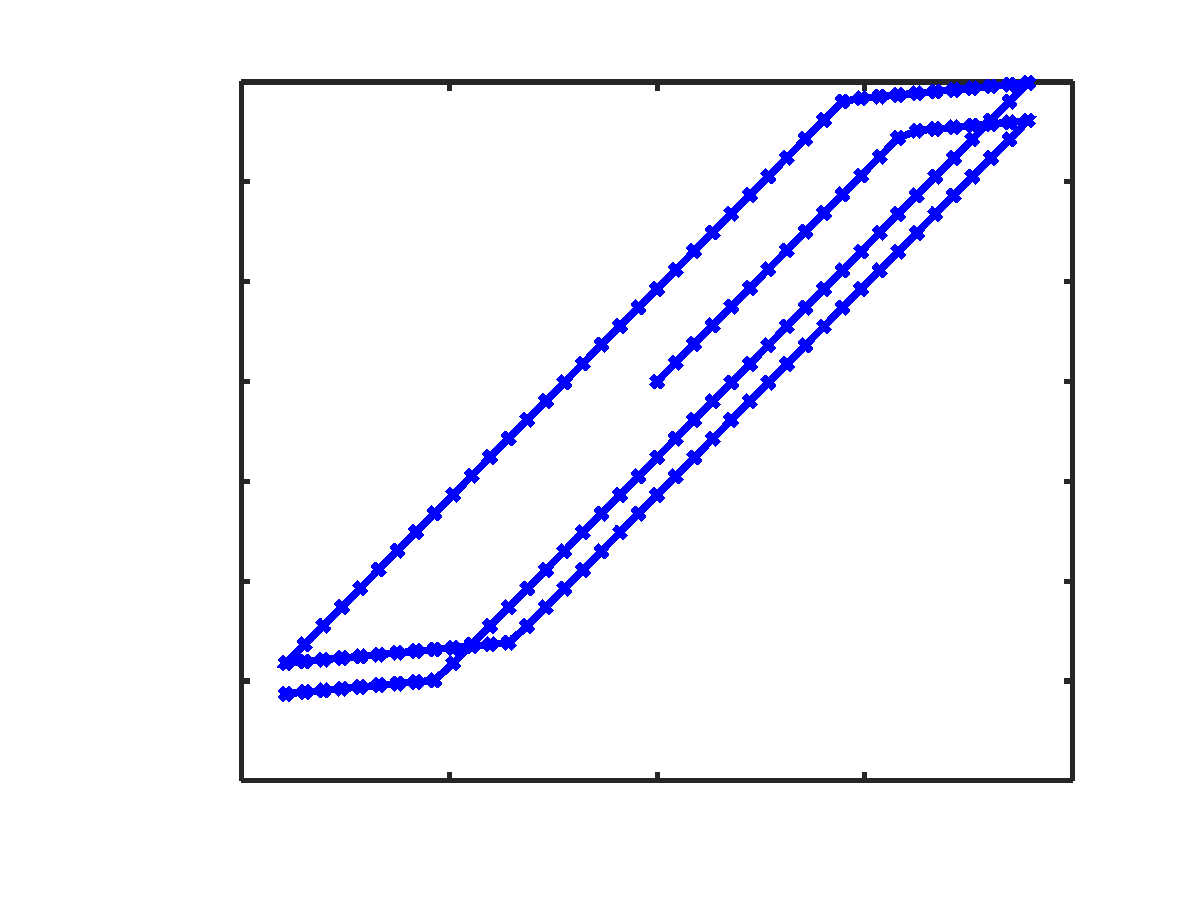
\includegraphics{plasticcycle2-inc}
\end{picture}%
\begin{picture}(560,420)(0,0)
\fontsize{20}{0}
\selectfont\put(107.997,48.007){\makebox(0,0)[t]{\textcolor[rgb]{0.15,0.15,0.15}{{-0.002}}}}
\fontsize{20}{0}
\selectfont\put(207.698,48.007){\makebox(0,0)[t]{\textcolor[rgb]{0.15,0.15,0.15}{{-0.001}}}}
\fontsize{20}{0}
\selectfont\put(307.399,48.007){\makebox(0,0)[t]{\textcolor[rgb]{0.15,0.15,0.15}{{0}}}}
\fontsize{20}{0}
\selectfont\put(407.099,48.007){\makebox(0,0)[t]{\textcolor[rgb]{0.15,0.15,0.15}{{0.001}}}}
\fontsize{20}{0}
\selectfont\put(506.8,48.007){\makebox(0,0)[t]{\textcolor[rgb]{0.15,0.15,0.15}{{0.002}}}}
\fontsize{20}{0}
\selectfont\put(103,52.9996){\makebox(0,0)[r]{\textcolor[rgb]{0.15,0.15,0.15}{{-4e+08}}}}
\fontsize{20}{0}
\selectfont\put(103,100.928){\makebox(0,0)[r]{\textcolor[rgb]{0.15,0.15,0.15}{{-3e+08}}}}
\fontsize{20}{0}
\selectfont\put(103,148.857){\makebox(0,0)[r]{\textcolor[rgb]{0.15,0.15,0.15}{{-2e+08}}}}
\fontsize{20}{0}
\selectfont\put(103,196.785){\makebox(0,0)[r]{\textcolor[rgb]{0.15,0.15,0.15}{{-1e+08}}}}
\fontsize{20}{0}
\selectfont\put(103,244.714){\makebox(0,0)[r]{\textcolor[rgb]{0.15,0.15,0.15}{{0}}}}
\fontsize{20}{0}
\selectfont\put(103,292.643){\makebox(0,0)[r]{\textcolor[rgb]{0.15,0.15,0.15}{{1e+08}}}}
\fontsize{20}{0}
\selectfont\put(103,340.571){\makebox(0,0)[r]{\textcolor[rgb]{0.15,0.15,0.15}{{2e+08}}}}
\fontsize{20}{0}
\selectfont\put(103,388.5){\makebox(0,0)[r]{\textcolor[rgb]{0.15,0.15,0.15}{{3e+08}}}}
\fontsize{20}{0}
\selectfont\put(307.399,24.007){\makebox(0,0)[t]{\textcolor[rgb]{0.15,0.15,0.15}{{Deformacion}}}}
\fontsize{20}{0}
\selectfont\put(23.9999,220.75){\rotatebox{90}{\makebox(0,0)[b]{\textcolor[rgb]{0.15,0.15,0.15}{{Tension}}}}}
\end{picture}
}
	\caption{Gráficos tensión-deformación de ejemplos de comportamiento elastoplástico: modelo elastoplástico perfecto (izq.) y modelo con endurecimiento lineal (der.).}
	\label{fig:grafsplast}
\end{figure}

Se observa, como era de esperar, que la tensión va aumentando conforme continúa el proceso de carga descarga. %
%
Esto es explicado por el hecho de que a pesar de que la deformación total se mantenga acotada, la deformación plástica acumulada durante el proceso continua aumentando. %
%
Si los resultados experimentales o el modelo constitutivo del material establecen algún valor de tensión de rotura, el mismo podría ser alcanzado luego de un cierto número de ciclos.

\subsection{Aplicación a reticulados}

El desarrollo presentado anteriormente puede ser aplicado al análisis de estructuras formadas por elementos con comportamiento elasto-plástico. %
%
Para esto, se debe incluir el cálculo de las magnitudes asociadas a la plastificación dentro de los algoritmos iterativos para encontrar la configuración de equilibrio. %
%
En el primer capítulo de \citep{Simo1998} se encuentra un desarrollo completo de los modelos unidimensionales y su integración en algoritmos basados en el MEF.

\section[Solicitaciones últimas en sección de hormigón armado] {Ejemplo: cálculo de solicitaciones últimas en sección de hormigón armado} 
%

En esta sección se presenta una breve discusión sobre análisis no lineal de secciones y se resuelve un ejemplo de cálculo de solicitaciones últimas en una sección de hormigón armado considerando el comportamiento no lineal del hormigón. %

A pesar de que el comportamiento del hormigón es usualmente considerado elastoplástico, en el ejemplo se considera un análisis elástico no lineal dado por una relación tensión-deformación sin calcular deformaciones plásticas. %
%
En el caso de que no se realice descarga este análisis elástico no lineal produce resultados iguales a los del análisis utilizando el modelo de elastoplasticidad. %
%
En el caso de que la estructura no se lleve a la falla, es decir que continúe en servicio luego de la descarga, este análisis no es útil, ya que se deben calcular o estimar las deformaciones remanentes correspondientes.

Es importante resaltar que este tipo de análisis no es un análisis no lineal completo de un elemento estructural. %
%
Para realizar un análisis no lineal de un elemento de viga se debe considerar la no linealidad no solamente en la sección transversal sino que también según el eje de la viga. %
%
En \citep{Liew2017,Lemes2017} se presentan resultados de análisis no lineales de elementos de viga de acero y hormigón considerando la relación momento-curvatura dada por el comportamiento constitutivo. %
%
Utilizando un procedimiento similar al presentado en este ejemplo es posible construir el diagrama momento-curvatura de una sección de hormigón considerando efectos de complejidad de modelado como por ejemplo fisuración. %
%
En \citep{Alhasawi2017} se realiza un análisis de pórticos considerando elementos de viga con rótulas elasto-plásticas en los extremos, aplicando conceptos de plasticidad como los vistos en la sección anterior.


En el ejemplo desarrollado a continuación se calculan los momentos y directas integrando el diagrama de tensiones de la sección utilizando integración numérica. %
%
Para la integración se utiliza el método de cuadratura de Gauss \citep{quarteroni2007numeric}, el cual permite calcular de forma eficiente las solicitaciones tal como se muestra en \citep{Bonet2006}.

Se considera una sección de hormigón armado de geometría rectangular de ancho $b=0.25$ m y altura $h= 0.6$ m con armadura simétrica dispuesta como se muestra en la Figura~\ref{fig:seccion}, con recubrimiento mecánico $r_m=0.06$ m. %
%
Los rectángulos oscuros representan barras de acero de refuerzo.
	
%
\begin{figure}[htb]
	\def\svgwidth{0.4\textwidth}
\input{../fig/seccion.pdf_tex}
	\caption{Esquema de sección transversal de hormigón armado.}
	\label{fig:seccion}
\end{figure}

El acero considerado es de tipo B500 y el hormigón es tipo C25 (resistencia característica $f_{ck}=25 $ N/mm$^2$). %

Se desea obtener las solicitaciones últimas resistidas por la sección para diferente cuantía, posición de linea neutra y curvatura, es decir los diagramas de interacción para la sección.

Para la resolución de este ejemplo nos guiaremos por el procedimiento descrito en \citep{JimenezMontoya}, material basado en la norma española EHE-2008\footnote{Enlace a norma en \href{http://www.fomento.es/MFOM/LANG_CASTELLANO/ORGANOS_COLEGIADOS/MASORGANOS/CPH/instrucciones/EHE_es/}{sitio web de ministerio de fomento español} (último acceso diciembre 2017).}. %
%
Para determinar las solicitaciones últimas soportadas por una sección rectangular se debe calcular las siguientes integrales
%
\begin{equation}
M_{\text{int}} = M_{\text{int}}^C + M_{\text{int}}^D = \int_{-\frac{h}{2}}^{\frac{h}{2}} b \, \sigma_x(y) \, y \, dy + \sum_{i=1}^{n_D} \sigma(y_i) \, y_i \, A_i 
\end{equation}
%
donde $M^C$ es el momento último dado por el hormigón (tensión continua en la altura) y $M^D$ es el momento producido por tensiones discretas (barras), $y_i$ y $A_i$ son las posiciones y áreas donde hay barras de acero, e $y$ vale cero en la mitad de la altura. %
%

Se considera además $y_1=-0.45h$, $y_2=0.45h$ y armadura simétrica ($A_1 = A_2 = A_s$). %

De forma análoga se calcula la directa resultante:
%
\begin{equation}  
N_{\text{int}} = N_{\text{int}}^C + N_{\text{int}}^D = \int_{-\frac{h}{2}}^{\frac{h}{2}} b \, \sigma_x(y) \,  dy + \sum_{i=1}^{n_{D}} \sigma(y_i) \, A_i 
\end{equation}
%

Pueden ser fácilmente implementadas funciones de Octave que permitan calcular los valores de directa y momento a partir de la curvatura y la posición de la linea neutra. %
%
A partir de dichas funciones, se pueden calcular las integrales numéricamente utilizando el método de cuadratura de Gauss, en este caso con cinco puntos de integración. %

Las integrales se calculan evaluando el integrando que depende de la función $\sigma(y)$. %
%
Esta función $\sigma(y)$ está dada a través de la ecuación constitutiva axial y la expresión de la deformación, es decir $\sigma (y) = \sigma( \varepsilon ( y) )$. %

La función de deformación en función de la distancia a la línea neutra  $y - y_{N}$ y la curvatura $\kappa$ se puede expresar de la siguiente forma:
%
\begin{equation}
\varepsilon(y) = - \kappa \, (y - y_{N} ) 
\end{equation}
%
donde $y_N$ es la posición de la linea neutra.

La ecuación constitutiva considerada para el hormigón es del tipo parábola-rectángulo, sin considerar resistencia a tracción, mientras que para el acero se utiliza un modelo elastoplástico perfecto. %
%
La expresión analítica de la ecuación constitutiva del hormigón es:
%
\begin{equation}
\sigma^C(\varepsilon) = %
\left\{ %
\begin{array}{lcl}
-f_{cd}  & \text{ si } & \varepsilon  \in [ -3.5 \text{\permil} , -2\text{\permil} ]  \\[2mm]
1000  \,.\, f_{cd}  \,.\, \varepsilon  \,.\, ( 250 \,.\, \varepsilon + 1)  & \text{si} & \varepsilon \in [  -2 \text{\permil} , 0] \\[2mm]
0  & \text{ si } & \varepsilon  > 0 \\[2mm]
\end{array}   \right.
\end{equation}
%
mientras que para el acero se tiene que la tensión de límite elástico es $\varepsilon_y = 2.17 \text{\permil}$ y por lo tanto la ecuación está dada por
%
\begin{equation}
\sigma^D(\varepsilon) = %
\left\{ %
\begin{array}{lcl}
E \, \varepsilon  & \text{si} & |\varepsilon| < 2,17 \text{\permil} \\[2mm]
f_{yd} \,. \, \text{signo}(\varepsilon) \quad & \text{si} & |\varepsilon| \geq 2,17 \text{\permil} \\[2mm]
\end{array}   \right.
\end{equation}
%
%Los códigos de las funciones de octave utilizados para evaluar estas funciones están presentados en la Sección~\ref{sec:cod2}. %

Las relaciones constitutivas del hormigón y el acero son representadas gráficamente en la Figura~\ref{fig:graficos_consitutivas} a la izquierda y derecha respectivamente.
%
\begin{figure}[htb]
	\centering
\def\svgwidth{0.95\textwidth}
\input{../fig/graficos_consitutivas.pdf_tex}
		\caption{Relaciones constitutivas de hormigón (izquierda) y acero (derecha).} \label{fig:graficos_consitutivas}
\end{figure}

Finalmente, se calculan las solicitaciones para los valores de linea neutra y curvatura dados por el diagrama de pivotes y con los valores obtenidos se construye el diagrama de interacción mostrado en la Figura~\ref{fig:interaccion}.

\setlength{\unitlength}{0.95\textwidth}
\begin{figure}[htb]
	\noindent
	\begin{center}
		\begin{picture}(1,0.75)%
		\put(0,0){\includegraphics[width=\unitlength]{../fig/interaccion.pdf}}%
		\put(0.75,0.6){\color[rgb]{0,0,0}\makebox(0,0)[lb]{\smash{$\mu=\dfrac{M}{b h^2 f_{cd}}$}}}%
		\put(0.75,0.5){\color[rgb]{0,0,0}\makebox(0,0)[lb]{\smash{$\nu=\dfrac{N}{b h f_{cd}}$}}}%
		\put(0.75,0.4){\color[rgb]{0,0,0}\makebox(0,0)[lb]{\smash{$\omega = \dfrac{A f_{yd} }{b h f_{cd}}$}}}%
		\end{picture}%
		\caption{Diagrama de interacción de sección rectangular de hormigón armado.} \label{fig:interaccion}
	\end{center}
\end{figure}

Los ejes del gráfico muestran los momentos y directas reducidos, $\mu$ y $\nu$ respectivamente y las líneas punteadas conectan los puntos $(\nu,\mu)$ en los cuales se produce el cambio de dominio en el diagrama de pivotes para las distintas cuantías consideradas.

\cajaactividad{Comparar el diagrama de interacción obtenido con el correspondiente presentado en \citep{JimenezMontoya}.}

 % Autor JPZ. Material Hiperelástico NoLin. Plasticidad.

% ------ Capitulo 4 - Dinamica ---------
%\chapter{Introducción al Análisis Dinámico}\label{cap4DIN}

En capítulos anteriores se cubrió el análisis de estructuras en régimen no lineal bajo la hipótesis de una respuesta estática. Un gran número de problemas prácticos requieren la capacidad de realizar análisis dinámicos de estructuras, se enumeran algunos a modo de ejemplo:
%
\begin{itemize}
	\item puentes y estructuras sometidas a cargas de tránsito dinámicas de tipo peatonal, carretero, ferroviario u otro,
	\item estructuras de soporte y/o fundaciones para maquinaria recíprocante o vibratoria,
	\item estructuras sometidas a movimientos sísmicos,
	\item impactos sobre estructuras,
	\item estructuras sometidas a explosiones.
\end{itemize}
%
Surge por lo tanto la necesidad de abandonar la hipótesis de carga estática y considerar el análisis dinámico de estructuras en régimen no lineal.

En este capítulo no se intenta cubrir el contenido de un curso de dinámica estructural, por el contrario, se busca únicamente sentar las bases de la resolución de problemas de dinámica no lineal, con lo cual, se omitirán conocimientos básicos de dinámica. %
%
Un libro recomendable para repasar dichos conocimientos básicos es \citep{clough1993dynamics}. %
%
La presentación que aquí se realiza está basada en los capítulos 9 y 24 de los libros \citep{Bathe2014} y \citep{Crisfield1997} respectivamente.

El presente capítulo consta a grandes rasgos de tres secciones. La primera presenta el planteo de las ecuaciones de movimiento de la estructura y describe sus componentes. La segunda sección presenta métodos de análisis dinámico y ejemplos para estructuras en régimen lineal. Finalmente, la tercera sección refiere a procedimientos de solución y ejemplos de estructuras no lineales.



\section{Deducción de las Ecuaciones de Movimiento}\label{EcMov}

Continuando con el material presentado en el Capítulo 2, se plantea a continuación la condición de equilibrio dinámico de una estructura compuesta por barras axiales con grandes desplazamientos y rotaciones pero pequeñas deformaciones unitarias.

En este contexto, se recurre al Principio de D'Alambert para establecer las ecuaciones de movimiento de un elemento de barra axial. Dicho principio es el equivalente dinámico al PTV. El mismo incorpora las fuerzas inerciales como fuerzas externas y permite expresar el equilibrio dinámico en forma variacional equivalente al PTV.

En lo que sigue, se hace referencia al tiempo mediante la variable independiente $t$ y se definen todas las variables estructurales (posición, desplazamiento, deformación unitaria, tensión, etc) como función del tiempo ($\bfx_t$, $\bfu_t$, $\sigma_t$, etc). %
%
Se utilizará la siguiente notación para expresar derivadas primera y segunda respecto del tiempo: $\dot{\bfu}_t$ y $\ddot{\bfu}_t$.

Dado lo anterior, para una barra axial, el Principio de D'Alambert sostiene que $\forall t$ y $\forall \delta \bfu \in \mcV$ se cumple:
%
\begin{equation}\label{DALAMBERT}
	\int_{V_t} \sigma_t \delta \varepsilon \dif V_t 
	= \int_{V_t}  \delta \bfu^\text{T} \bfb_{\text{ext},t} \, \dif V_t  - \int_{V_t} \rho_t \delta \bfu^\text{T} \ddot{\bfu}_t  \dif V_t - \int_{V_t} c \delta \bfu^\text{T} \dot{\bfu}_t  \dif V_t,
\end{equation}
%
donde $\bfb_{ext,t}$ representa el campo vectorial de fuerzas externas de volumen. %
%
Notar que, en la Ecuación~\eqref{DALAMBERT}, los vectores de desplazamiento $\bfu_t$ pertenecen a $\bbR^3$ que representan desplazamentos de partículas y no desplazamientos nodales.
 
En la Ecuación~\eqref{DALAMBERT}, la primer integral del miembro derecho corresponde a las fuerzas inerciales, siendo $\rho$ la densidad del material. Por otro lado, la segunda integral del miembro derecho corresponde a fuerzas viscosas disipativas, siendo $c>0$ un factor de disipación arbitrario.


La disipación viscosa presentada en este contexto es un mecanismo artificial para introducir efectos de amortiguamiento estructural. %
%
La misma no tiene, en general, un significado físico directo y por ende la disipación no se determinará usando una expresión teórica para $c$, sino que se realizará por medios empíricos. %
% -----------------

Aplicando una discretización de elementos finitos como la utilizada en el Capítulo 2 en la Ecuación~\eqref{DALAMBERT} y mediante consideraciones ya discutidas sobre el volumen de la barra para pequeñas deformaciones unitarias, se llega a la siguiente ecuación de movimiento a nivel de estructura:
%
\begin{equation}\label{EcMovNL}
	\bff_{\text{int}}(\bfu_t) = \bff_{\text{ext},t} - \bfM \ddot{\bfu}_t - \bfC \dot{\bfu}_t.
\end{equation}

Las cargas dinámicas externas están dadas por el vector $\bff_{\text{ext},t}$ y pueden ser periódicas (harmónicas, no harmónicas) o aperiódicas (impulsivas, transitorias). %
%
El tipo de carga influye en la definición del modelo estructural y a su vez en el método de resolución de las ecuaciones de movimiento resultantes.

El vector de fuerzas internas $\bff_{\text{int}}$ incorpora los efectos de no linealidad geométrica y eventualmente otros tipos de comportamiento no lineal de los elementos de barra, como puede ser la no linealidad material.

La matriz $\bfM$ es llamada Matriz de Masa. %
%
Si ésta se deduce usando las funciones de interpolación de $\bfu$ en la formulación de elementos finitos, se le suele llamar Matriz de Masa Consistente. Por el contrario, si es deducida concentrando la masa del elemento en sus nodos y asignándola a sus respectivos grados de libertad de desplazamiento, se la llama Matriz de Masa Concentrada. %
%
En este documento se consideran matrices de masa concentrada. %
%
Se puede verificar que los resultados obtenidos usando una u otra matriz son prácticamente equivalentes con una discretización suficientemente fina de elementos.

A modo de ejemplo se presenta la matriz de masa concentrada para el elemento de barra bi-dimensional:
%
\begin{equation}
\bfM^e = \frac{\rho A \ell_0}{2}
\left[\begin{matrix}
1 & 0 & 0 & 0\\
0 & 1 &0 & 0\\
0 & 0& 1 & 0\\
0 & 0 &0 & 1\\
\end{matrix}
\right]
\end{equation}

La matriz $\bfC$ es llamada Matriz de Amortiguamiento y permite incorporar los efectos disipativos viscosos de la estructura. %
%
Tal como fue indicado anteriormente, es habitual elegir una matriz $\bfC$ tal que de la aplicación de dicha matriz se obtengan amortiguamientos cercanos a valores empíricos conocidos para estructuras similares a la considerada. %
%
Por ejemplo, si se estudia una estructura metálica soldada y se sabe que una estructura de fabricación similar exhibió un cierto porcentaje del amortiguamiento crítico bajo vibraciones a ciertas frecuencias, se intentará elegir una matriz $\bfC$ que reproduzca esas características de amortiguamiento.

Una formulación usual para la matriz $\bfC$ es un tipo de amortiguamiento proporcional conocido como amortiguamiento de Rayleigh, ver \citep{clough1993dynamics}:
%
\begin{equation} \label{eqn:amorRayl}
	\bfC = \eta \bfM + \chi \bfK.
\end{equation}

Esta matriz de amortiguamiento permite fijar valores aproximados de amortiguamiento para ciertos rangos de frecuencias y tiene la ventaja de ser esparza, al igual que $\bfK$. %
%
Es claro que otros tipos de amortiguamiento pueden ser incorporados mediante la matriz $\bfC$, por ejemplo amortiguadores conectados a dos nodos dados de la estructura. %
%
En estas situaciones se puede perder la característica de amortiguamiento proporcional.





\section{Dinámica Lineal}\label{DinLin}

Tal como fue mencionado, previo al abordaje de conceptos de dinámica no lineal, se presentará el problema y métodos de análisis de dinámica lineal. %
%

En esta sección se introducen dos métodos de integración directa de las ecuaciones de movimiento de uso habitual en la práctica. %
%
El primero de ellos es un método explícito, condicionalmente estable, llamado Método de Diferencia Centrada y el segundo es un método implícito, incondicionalmente estable bajo ciertas hipótesis, llamado Método de Newmark.


Antes de introducir los métodos, es conveniente escribir la ecuación de movimiento (ver Ecuación~\eqref{EcMovNL}) en la hipótesis de comportamiento lineal. %
%
Para ello, se asumen pequeñas deformaciones y desplazamientos y comportamiento material elástico lineal, de lo cual resulta una matriz de rigidez lineal $\bfK$ a nivel de estructura como la vista en cursos de elementos finitos lineales. %
%
En el caso de los elementos de barra vistos en el Capítulo 2, la matriz lineal del elemento corresponde a $\bfK^e=E A_0 \ell_0 \bfb_1^\text{T} \bfb_1$. %
%
Sea $\alpha$ el ángulo que forma la barra con la horizontal y llamando $c=\cos(\alpha)$ y $s=\sin(\alpha)$, se obtiene:
%
\begin{equation}
\bfK^e = \frac{E A}{\ell_0}
\left[\begin{matrix}
c^2 & c s & -c^2 & -c s\\
c s & s^2 & -c s & -s^2\\
-c^2 & -c s & c^2 & c s\\
-c s & -s^2 & c s & s^2\\
\end{matrix}
\right].
\end{equation}

Dado lo anterior, el vector de fuerzas internas $\bff_{\text{int}}(\bfu_t)$ está dado por $\bfK \bfu_t$, por lo que la ecuación de movimiento para el análisis dinámico lineal de la estructura resulta:
%
\begin{equation}\label{EcMovLin}
	\bfM \ddot{\bfu}_t + \bfC \dot{\bfu}_t + \bfK \bfu_t = \bff_{\text{ext},t}
\end{equation}

La Ecuación~\eqref{EcMovLin} representa un sistema de ecuaciones diferenciales ordinarias de segundo grado, con coeficientes constantes y no homogéneas. Para determinar una solución, se deben dar condiciones iniciales en el instante $t_0$ de desplazamiento ($\bfu_{t_0}$) y velocidad ($\dot{\bfu}_{t_0}$).

Las definiciones de las matrices $\bfM$ y $\bfC$, junto con comentarios generales sobre las mismas, ya fueron presentadas en la sección anterior y mantienen su validez.


\subsection{Método de Diferencia Centrada - Explícito}

El Método de Diferencia Centrada, presentado en esta sección, es probablemente el más sencillo entre los métodos de integración directa de las ecuaciones de movimiento. %
%
Por otra parte, este método puede resultar computacionalmente muy económico para ciertos modelos de elementos finitos y tipos de cargas dinámicas. 


Se verá más adelante que el método solamente requiere conocer la solución de la ecuación de movimiento en un instante de tiempo dado $t$ para poder determinar, mediante la evaluación de una expresión explícita, la solución en un tiempo posterior $t+\Delta t$. %
%
Esta característica es la que define a la clase de métodos \textit{explícitos}. %
%
Estos métodos son especialmente adecuados para resolver problemas dinámicos con transitorios rápidos, como ser el análisis de estructuras sometidas a impacto, explosiones o propagación de ondas.

A modo de ejemplo, el software \textit{Abaqus Explicit} utiliza este método de solución y permite modelar problemas del tipo indicado en el párrafo anterior\footnote{ver sitio web de \textit{Dassault Systèmes}\textsuperscript{\textregistered}.}. %
%
La formulación es levemente distinta a la presentada aquí, pero el método es el mismo.

\subsubsection{Formulación y Pseudo-código}

La formulación del método se basa en utilizar las siguientes aproximaciones de las derivadas de los desplazamientos, las cuales están basadas en diferencias centradas. Estas aproximaciones corresponden a las velocidades
%
\begin{equation}\label{DifCenVel}
\dot{\bfu}_t \simeq \frac{\bfu_{t+\Delta t}-\bfu_{t-\Delta t}}{2\Delta t},
\end{equation}
y aceleraciones
\begin{equation}\label{DifCenAccel}
	\ddot{\bfu}_t \simeq \frac{\bfu_{t+\Delta t}-2\bfu_{t}+\bfu_{t-\Delta t}}{\Delta t ^2}.
\end{equation}

Se asume que se conoce la solución hasta el instante $t$ y que, dado un incremento en el tiempo $\Delta t$, se desea hallar la solución en el instante $t+\Delta t$. %
%
Con lo cual, la incógnita a determinar es $\bfu_{t+\Delta t}$.

Para completar la definición del método, se debe utilizar la ecuación de movimiento. %
%
En particular, se considera el equilibrio dinámico en el instante $t$, dado por la Ecuación~\eqref{EcMovLin} y se sustituyen las expresiones aproximadas para la aceleración y la velocidad, dadas por las Ecuaciones \eqref{DifCenAccel} y \eqref{DifCenVel}. %
%
Realizando esto se obtiene:
%
\begin{equation}
\bfM \left[\frac{\bfu_{t+\Delta t}-2\bfu_{t}+\bfu_{t-\Delta t}}{\Delta t ^2}\right] + \bfC \left[\frac{\bfu_{t+\Delta t}-\bfu_{t-\Delta t}}{2\Delta t}\right] + \bfK \bfu_t = \bff_{\text{ext},t}.
\end{equation}

Despejando el desplazamiento incógnita $\bfu_{t+\Delta t}$ se llega a que:
%
\begin{equation}\label{EcDifCent}
\begin{split}
	\left[\frac{1}{\Delta t^2}\bfM + \frac{1}{2\Delta t}\bfC \right] \bfu_{t+\Delta t} = \bff_{\text{ext},t} - & \left[\bfK-\frac{2}{\Delta t ^2}\bfM\right] \bfu_t \\
	-& \left[\frac{1}{\Delta t^2}\bfM-\frac{1}{2\Delta t}\bfC\right] \bfu_{t-\Delta t}
\end{split}
\end{equation}

Notar que en este método se aproximan las aceleraciones y velocidades en el instante $t$, este error suele llamarse error de truncamiento en referencia al truncamiento de una serie de Taylor. %
%
Cabe observar que este error de truncamiento puede ser reducido eligiendo un paso temporal $\Delta t$ más pequeño. %
%
En segundo lugar, se introduce otro error al determinar la solución en el tiempo $t+\Delta t$ a partir del equilibrio dinámico en el instante $t$. Es inmediato ver que las aceleraciones, velocidades y desplazamientos del tiempo $t+\Delta t$ hallados mediante este método no satisfarán exactamente la ecuación de movimiento en el tiempo $t + \Delta t$.

En el Algoritmo~\ref{PCDifCent} se presenta un Pseudo-Código del método.

\begin{algorithm}[htb]
\caption{Método de Diferencia Centrada.} \label{PCDifCent}
	\begin{algorithmic}[1]
	\STATE Ensamblar: $\bfM$, $\bfK$ y $\bfC$ a nivel de estructura.
	\STATE Definir: tiempo final de análisis dinámico: $t_f$
	\STATE Definir: Condiciones iniciales: $\bfu_{0}$, $\dot{\bfu}_{0}$
	\STATE Calcular: $\ddot{\bfu}_{0}\leftarrow \bfM^{-1}(\bff_{ext,t} - \bfC \dot{\bfu}_0 - \bfK \bfu_0)$
	\STATE Definir: $\Delta t$ tal que $\Delta t < T_{min} / \pi$
	\STATE Calcular: $a_0\leftarrow1/\Delta t^2$, $a_1\leftarrow1/(2\Delta t)$, $a_2\leftarrow2a_0$ y $a_3\leftarrow1/a_2$
	\STATE Calcular: $\bfu_{-\Delta t} \leftarrow \bfu_0 - \Delta t \dot{\bfu}_0 + a_3\ddot{\bfu}_0$
	\STATE Calcular y factorizar: $\hat{\bfM}\leftarrow a_0\bfM+a_1\bfC$
	\STATE $t \leftarrow 0$
	\WHILE{$t<t_f$}
		\STATE Calcular: $\hat{\bff}_t\leftarrow \bff_{ext,t} - (\bfK-a_2\bfM)\bfu_t - (a_0\bfM-a_1\bfC)\bfu_{t-\Delta t}$
		\STATE Resolver: $\bfu_{t+\Delta t}\leftarrow \hat{\bfM}^{-1}\hat{\bff}_t$
		\STATE Calcular aceleración: $\ddot{\bfu}_{t}\leftarrow a_0(\bfu_{t+\Delta t}-2\bfu_{t}+\bfu_{t-\Delta t})$
		\STATE Calcular velocidad: $\dot{\bfu}_{t}\leftarrow a_1(\bfu_{t+\Delta t}-\bfu_{t-\Delta t})$
		\STATE $t\leftarrow t+\Delta t$
	\ENDWHILE	
\end{algorithmic}
\end{algorithm}

Analizando la línea 12 del Pseudo-Código se puede ver que este método puede ser extremadamente económico desde el punto de vista computacional si la matriz $\hat{\bfM}$ es invertible de manera económica, particularmente si esta matriz es diagonal. %
%
Es por esto que al aplicar este método se utiliza la matriz de Masa Concentrada y no la matriz de Masa Consistente. %
%
Adicionalmente, la matriz de efectos viscosos puede ser despreciada en fenómenos rápidos de muy corta duración. %
%
En su defecto, se utiliza una matriz $\bfC$ diagonal de manera de no aumentar el costo computacional.


\subsubsection{Estabilidad Numérica}\label{DifCenStab}

En el Algoritmo~\ref{PCDifCent} se indica que el valor del paso temporal elegido debe satisfacer la condición: $\Delta t < T_{min}/\pi$, donde $T_{min}$ es el mínimo período de vibración natural del modelo de elementos finitos. Para entender esta restricción, se realiza el análisis de la estabilidad numérica del Método de Diferencia Centrada.

El análisis de estabilidad numérica se lleva a cabo en una estructura sin amortiguamiento, es decir con $\bfC = 0$. Sin embargo, es posible analizar la estabilidad tomando en cuenta el amortiguamiento, en particular bajo la hipótesis de amortiguamiento proporcional. %
%
Se realizará algún comentario adicional a este punto más adelante en esta sección.

Previo a realizar el análisis de estabilidad numérica, se debe reconocer que es suficiente estudiar la estabilidad de la solución numérica de un sistema con un grado de libertad. %
%
La justificación de este hecho se basa en la descomposición modal de la respuesta de la estructura y se describe brevemente a continuación.

Se definen los modos normales de vibración de la estructura como aquellas soluciones de vibración libre no forzada en las que todos los puntos de la estructura se desplazan de forma sinusoidal respecto del tiempo, en fase y a una misma frecuencia; es decir: $\bfu_t = \sin(\omega(t-t_0)) \bfphi $, donde $\bfphi$ es un vector de desplazamientos nodales asociados a las amplitudes del movimiento.

Sustituyendo el modo normal definido anteriormente en la ecuación de movimiento (sin amortiguamiento ni fuerzas externas) se obtiene la siguiente relación:
%
\begin{equation}
	\omega^2 \bfM \bfphi = \bfK \bfphi.
\end{equation}

La ecuación anterior define un problema de valores propios para una matriz simétrica definida positiva. Esto implica que existen tantos modos normales \{$\bfphi_i$ , $\omega_i^2$\} como grados de libertad tenga la estructura ($n$), es decir tantos como la dimensión de las matrices $\bfM$ o $\bfK$ (reducidas). %

\cajaactividad{Mostrar que los modos normales de vibración satisfacen la relación:
	$$\bfphi_i^T\bfM \bfphi_j = \delta_{ij} \quad i,j=1,\dots,n,
	$$
	donde $\delta_{ij}$ es el delta de Kronecker.}

Agrupando cada uno de los $n$ modos normales $\bfphi_i$ como columnas de una matriz $\bfPhi$, y sus respectivas frecuencias al cuadrado ($\omega_i^2$) en la diagonal de una matriz $\bfLam$, se tiene:
%
\begin{equation}\label{ModosNormales}
\bfM \bfPhi \bfLam = \bfK \bfPhi
\end{equation}

La Ecuación~\eqref{ModosNormales} define la relación matricial que verifican los modos normales de la estructura. Queda definida así una base de vectores dada por $\bfPhi$ en la cual se pueden escribir los vectores de desplazamiento a lo largo del tiempo.

A partir del desarrollo anterior, se define $\bfu_t = \bfPhi \bfx_t$. Es decir, $\bfx_t$ son las coordenadas que representan a $\bfu_t$ en la base de modos normales $\bfPhi$. La ecuación de movimiento resulta:
%
\begin{equation}\label{EcMovDiag1}
	\bfM \bfPhi \ddot{\bfx}_t + \bfK \bfPhi \bfx_t = \bff_{\text{ext},t}.
\end{equation}

Si se multiplica la Ecuación~\eqref{EcMovDiag1} a la izquierda por $\bfPhi^T$ se obtiene,
%
\begin{equation}\label{EcMovDiag2}
\bfPhi^T \bfM \bfPhi \ddot{\bfx}_t + \bfPhi^T \bfK \bfPhi \bfx_t = \bfPhi^T \bff_{\text{ext},t}.
\end{equation}
%
Usando la condición de $\bfM$-ortonormalidad de los vectores $\bfphi_i$ y definiendo $\bfnu_t=\bfPhi^T \bff_{\text{ext},t}$ se llega a:
%
\begin{equation}\label{EcMovDiag}
\ddot{\bfx}_t + \bfLam \bfx_t = \bfnu_t.
\end{equation}

De la Ecuación~\eqref{EcMovDiag} se puede concluir que al cambiar la base a $\bfPhi$, la ecuación de movimiento queda diagonalizada o en otras palabras se desacoplan las ecuaciones de movimiento de los distintos grados de libertad. En la nueva base se tiene:
%
\begin{equation}
\ddot{x}_{i,t} + \omega^2_i x_{i,t} = \nu_{i,t} \quad  i=1...n.
\end{equation}

Un breve comentario respecto del amortiguamiento. Si se considera el amortiguamiento, el argumento anterior es válido solamente si se asume que la matriz de amortiguamiento $\bfC$ cumple que $\bfPhi^T \bfC \bfPhi$ es una matriz diagonal. %
%
Queda como ejercicio verificar lo anterior. %
%
En esos casos se llega a ecuaciones de movimiento desacopladas de la forma:
%
\begin{equation}\label{EcMovDiagAmor}
\ddot{x}_{i,t} + 2\xi_i\omega_i \dot{x}_{i,t} + \omega^2_i x_{i,t} = \nu_{i,t}
\end{equation}

Queda establecido que se puede analizar el comportamiento de la solución numérica de la ecuación de movimiento de un sistema de un grado de libertad sin amortiguamiento y considerando varias componentes se abarca el análisis de una estructura completa.

Se define por lo tanto el \textit{Problema Test} con el cual se analiza la estabilidad numérica del Método de Diferencia Centrada:
%
\begin{equation}\label{Ptest}
\text{Problema Test}
\begin{cases} 
\ddot{x}_t + \omega^2 x_t = 0\\
x_0 = 1 \\
\dot{x}_0 = 0\\
\end{cases}
\end{equation}

La aplicación del método de Diferencia Centrada al Problema Test resulta en la siguiente ecuación,
%
\begin{equation}\label{DifCent1DOF}
	x_{t+\Delta t} = (2-\omega_i^2 \Delta t^2)x_t - x_{t-\Delta t}.
\end{equation}

Se define el vector $\hat{\bfx}_{t+\Delta t} = [x_{t+\Delta t}, x_t]^T$. Usando la Ecuación~\eqref{DifCent1DOF} se puede presentar la solución con el método de Diferencia Centrada de la siguiente forma,
%
\begin{equation}\label{DifCentMatricial}
\hat{\bfx}_{t+\Delta t} = \bfA \hat{\bfx}_{t},
\end{equation}
donde la matriz $\bfA$ está definida como,
%
\begin{equation}\label{MatrizA}
\bfA = \left[\begin{matrix}
2-\omega_i^2 \Delta t^2 & -1 \\
1 & 0 \\
\end{matrix}
\right].
\end{equation}

El vector $\hat{\bfx}_{0}$ es un vector constante, no nulo, que queda definido a partir de las condiciones iniciales del Problema Test. %
%
Se puede suponer sin perder generalidad que $t=n \Delta t$ con $n\in \mathbb{N}$. Por lo tanto, la aplicación repetida de la Ecuación~\eqref{DifCentMatricial} permite obtener:
%
\begin{equation}\label{DifCentMatricial2}
\hat{\bfx}_{t} = \bfA^n \hat{\bfx}_{0}
\end{equation}

Es aquí que se impone el criterio de estabilidad numérica. Un sistema de un grado de libertad, sin amortiguamiento y sin forzamiento externo, que parte de una condición inicial dada tiene una solución oscilatoria que permanece acotada. Es natural por lo tanto, requerir que la solución numérica no diverja. Es decir que para todo instante $t$ se cumpla $\|\hat{\bfx}_t\|<\infty$.

Tomando normas en la Ecuación~\eqref{DifCentMatricial2} se obtiene la identidad:
%
\begin{equation}\label{MIM}
\|\hat{\bfx}_{t}\| = \|\bfA^n \hat{\bfx}_{0}\|.
\end{equation}

El miembro derecho de la Ecuación~\eqref{MIM} está acotado si, se cumple que el radio espectral de $\bfA$ es menor a 1, es decir $\rho(\bfA)<1$. %
%
El radio espectral de $\bfA$ se define como el máximo de los módulos de los valores propios de la matriz $\bfA$, es decir: $\rho(\bfA)=\max_i |\lambda_i|$. Si la multiplicidad de los valores propios es uno, la condición se puede relajar a $\rho(\bfA)\leq 1$.

La justificación formal de este punto se puede buscar en las notas del curso \textit{Métodos Numéricos} (Facultad de Ingeniería, \textit{Universidad de la República}). %
%
Alternativamente, un idea intuitiva de la validez de este resultado puede obtenerse pensando en que si $\bfA$ es diagonalizable ($\bfA = \bfP^{-1}\bfD \bfP$), entonces $\bfA^n = \bfP^{-1} \bfD^n \bfP$. Si los módulos de todos los valores propios que hay en la diagonal de $\bfD$ son menores a 1, se tiene que $\bfD^n\rightarrow 0$.

Por lo tanto, para evaluar la condición de estabilidad del método en cuestión debemos calcular los valores propios de $\bfA$, verificar que tienen multiplicidad igual a uno, e imponer que el módulo de éstos sea menor o igual a 1. 

Se define $z=\omega \Delta t>0$ con lo cual los valores propios resultan:
%
\begin{equation}\label{VProps}
\lambda_{1,2} = \frac{2-z^2}{2}\pm\sqrt{\frac{(2-z^2)^2}{4}-1}.
\end{equation}
%
Se puede ver que los valores propios tienen multiplicidad 1, incluso cuando $z=2$. %

En la Figura~\ref{fig:StabDifCentr} se presenta la gráfica de la función $\rho(\bfA)(z)=\max\{|\lambda_1(z)|,|\lambda_2(z)|\}$ para valores $z\in[0,3]$.

\begin{figure}[htb]
	\centering
	\resizebox{.58\linewidth}{!}{% Title: gl2ps_renderer figure
% Creator: GL2PS 1.4.0, (C) 1999-2017 C. Geuzaine
% For: Octave
% CreationDate: Sat May  8 08:49:58 2021
\setlength{\unitlength}{1pt}
\begin{picture}(0,0)
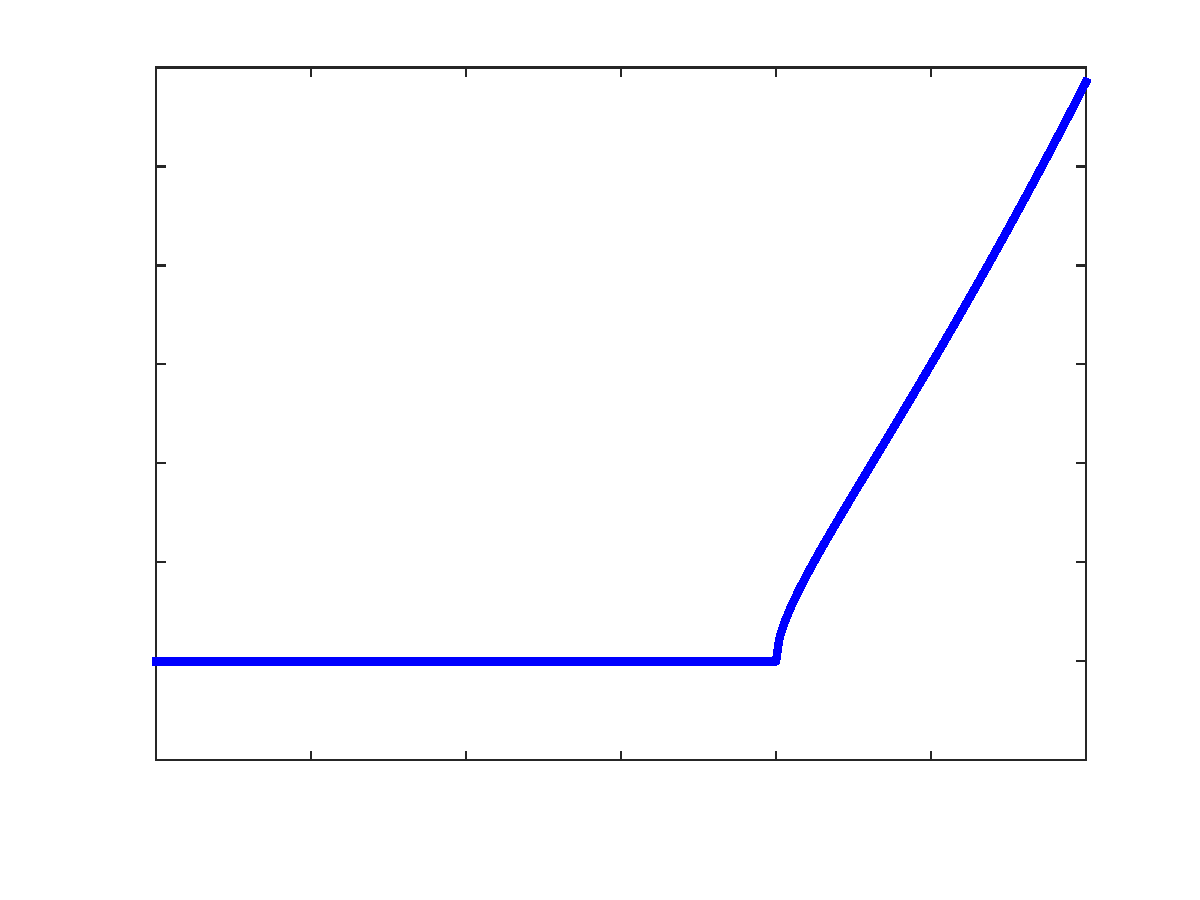
\includegraphics{Stabil-inc}
\end{picture}%
\begin{picture}(576,432)(0,0)
\fontsize{20}{0}
\selectfont\put(74.88,52){\makebox(0,0)[t]{\textcolor[rgb]{0.15,0.15,0.15}{{0}}}}
\fontsize{20}{0}
\selectfont\put(149.28,52){\makebox(0,0)[t]{\textcolor[rgb]{0.15,0.15,0.15}{{0.5}}}}
\fontsize{20}{0}
\selectfont\put(223.68,52){\makebox(0,0)[t]{\textcolor[rgb]{0.15,0.15,0.15}{{1}}}}
\fontsize{20}{0}
\selectfont\put(298.08,52){\makebox(0,0)[t]{\textcolor[rgb]{0.15,0.15,0.15}{{1.5}}}}
\fontsize{20}{0}
\selectfont\put(372.48,52){\makebox(0,0)[t]{\textcolor[rgb]{0.15,0.15,0.15}{{2}}}}
\fontsize{20}{0}
\selectfont\put(446.88,52){\makebox(0,0)[t]{\textcolor[rgb]{0.15,0.15,0.15}{{2.5}}}}
\fontsize{20}{0}
\selectfont\put(521.28,52){\makebox(0,0)[t]{\textcolor[rgb]{0.15,0.15,0.15}{{3}}}}
\fontsize{20}{0}
\selectfont\put(64.871,66.9828){\makebox(0,0)[r]{\textcolor[rgb]{0.15,0.15,0.15}{{0}}}}
\fontsize{20}{0}
\selectfont\put(64.871,114.499){\makebox(0,0)[r]{\textcolor[rgb]{0.15,0.15,0.15}{{1}}}}
\fontsize{20}{0}
\selectfont\put(64.871,162.016){\makebox(0,0)[r]{\textcolor[rgb]{0.15,0.15,0.15}{{2}}}}
\fontsize{20}{0}
\selectfont\put(64.871,209.533){\makebox(0,0)[r]{\textcolor[rgb]{0.15,0.15,0.15}{{3}}}}
\fontsize{20}{0}
\selectfont\put(64.871,257.05){\makebox(0,0)[r]{\textcolor[rgb]{0.15,0.15,0.15}{{4}}}}
\fontsize{20}{0}
\selectfont\put(64.871,304.566){\makebox(0,0)[r]{\textcolor[rgb]{0.15,0.15,0.15}{{5}}}}
\fontsize{20}{0}
\selectfont\put(64.871,352.083){\makebox(0,0)[r]{\textcolor[rgb]{0.15,0.15,0.15}{{6}}}}
\fontsize{20}{0}
\selectfont\put(64.871,399.6){\makebox(0,0)[r]{\textcolor[rgb]{0.15,0.15,0.15}{{7}}}}
\fontsize{22}{0}
\selectfont\put(298.08,32){\makebox(0,0)[t]{\textcolor[rgb]{0.15,0.15,0.15}{{$\omega_i \Delta t$}}}}
\fontsize{22}{0}
\selectfont\put(48.871,233.291){\rotatebox{90}{\makebox(0,0)[b]{\textcolor[rgb]{0.15,0.15,0.15}{{$\rho$}}}}}
\end{picture}
}
	\caption{Condición de Estabilidad del Método de Diferencia Centrada.}
	\label{fig:StabDifCentr}
\end{figure}

Se observa que se satisface el criterio de estabilidad si se cumple $\omega \Delta t \leq 2$. Llamando $T$ al período asociado a $\omega$, la condición es equivalente a: $\Delta t/ T \leq 1/\pi$.

En una estructura completa, todos los grados de libertad deben satisfacer esta condición. Se observa que la condición más estricta para $\Delta t$ corresponde al grado de libertad con el período natural más corto (es decir, el de mayor frecuencia), con lo cual el criterio de estabilidad numérica para una estructura completa es:
%
\begin{equation}
	\Delta t \leq \frac{T_{\text{min}}}{\pi},
\end{equation}
%
siendo $T_{\text{min}}$ el menor período natural.




\subsubsection{Ejemplo - Edificio Sometido a Carga de Explosión}\label{EjBlast}

Se considera la estructura de un edificio de hormigón armado con tres niveles, conformada por pilares, vigas y losas. %
%
La estructura considerada no representa una estructura realista, sino simplemente una idealización simplificada de un edificio. %

La geometría del edificio y la posición de la detonación considerada se muestra en la Figura~\ref{fig:Edificio} a través de una vista en planta (arriba) y un corte vertical (abajo).

\begin{figure}[htb]
	\centering
	\includegraphics[width=.9\linewidth]{../fig/edificio}
	\caption{Esquema de la Estructura del Edificio.}
	\label{fig:Edificio}
\end{figure}


Se considera que los pilares se empotran significativamente en los entrepisos y que los entrepisos son rígidos (a flexión y directa) en el plano. %
%
Con lo cual el movimiento lateral de la estructura en una dirección queda completamente definida por el desplazamiento lateral de cada piso ($u_1,u_2,u_3$) respecto de la posición original vertical. %
%
Esto permite realizar una idealización de la estructura a través de un modelo unidimensional mostrado en la Figura~\ref{fig:3dof}.

\begin{figure}[htb]
	\centering
	\includegraphics[width=.6\linewidth]{../fig/model3dof}
	\caption{Modelo del Edificio con 3 Grados de Libertad.}
	\label{fig:3dof}
\end{figure}

Dada la idealización estructural considerada, se plantea realizar el análisis dinámico lineal de la estructura. %
%
Se utiliza una matriz de masas concentradas, en la cual cada grado de libertad concentra la masa entre pisos adyacentes. Por otro lado, la matriz de rigidez se obtiene considerando la rigidez de un pilar empotrado-empotrado deslizante y la cantidad de pilares que se conectan a un entrepiso. Siendo $\bfu_t=[u_{1,t}, u_{2,t}, u_{3,t}]^T$,
%
\begin{equation}
\bfK = \frac{n_{cols} 12 E I }{H^3}
\left[\begin{matrix}
2 & -1 & 0 \\
-1 & 2 & -1 \\
0 & -1 & 1 \\
\end{matrix}
\right]
\end{equation}

La carga dinámica a la cual es sometido el edificio corresponde a las presiones generadas sobre la envolvente del edificio a causa de la detonación equivalente a 500 lbs de TNT a nivel de piso y a una distancia de 15m del edificio. Las presiones que se utilizan en el ejemplo fueron obtenidas del documento \citep{aisc2013guide26}.

Se resuelve la dinámica mediante el Método de Diferencia Centrada. La selección  del paso temporal $\Delta t$ se hizo considerando que se debía satisfacer la estabilidad numérica y que se debía capturar con suficiente precisión la súbita carga de presión de la explosión. %
%
El resultado del análisis numérico se muestra en la Figura~\ref{fig:blast}.

\begin{figure}[htb]
	\centering
	\resizebox{.9\linewidth}{!}{% Title: gl2ps_renderer figure
% Creator: GL2PS 1.4.0, (C) 1999-2017 C. Geuzaine
% For: Octave
% CreationDate: Fri Dec 29 11:50:59 2017
\setlength{\unitlength}{1pt}
\begin{picture}(0,0)
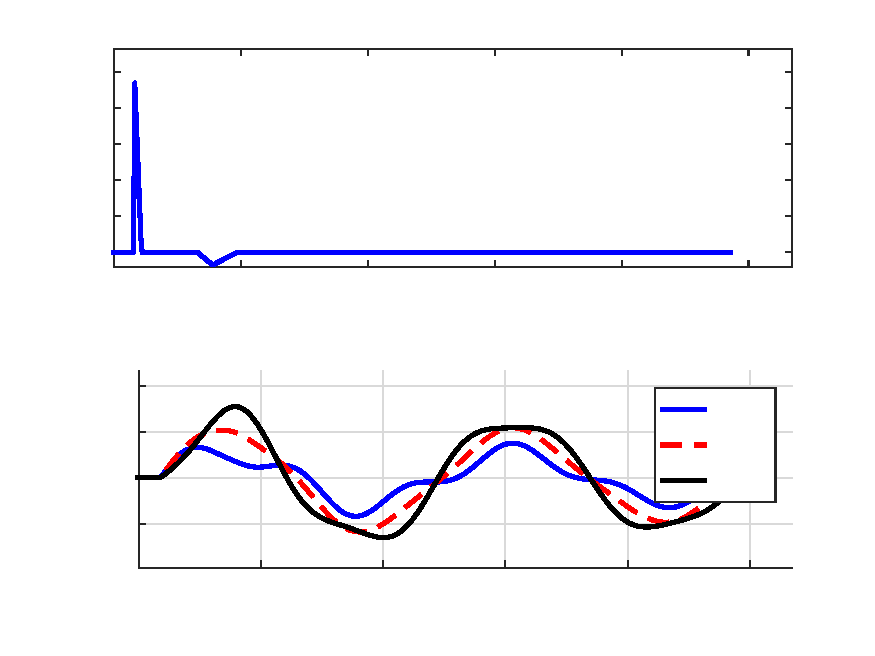
\includegraphics{Explicit-inc}
\end{picture}%
\begin{picture}(576,432)(0,0)
\fontsize{13}{0}
\selectfont\put(86.2902,42.5189){\makebox(0,0)[t]{\textcolor[rgb]{0.15,0.15,0.15}{{0}}}}
\fontsize{13}{0}
\selectfont\put(110.303,42.5189){\makebox(0,0)[t]{\textcolor[rgb]{0.15,0.15,0.15}{{0.02}}}}
\fontsize{13}{0}
\selectfont\put(134.315,42.5189){\makebox(0,0)[t]{\textcolor[rgb]{0.15,0.15,0.15}{{0.04}}}}
\fontsize{13}{0}
\selectfont\put(158.328,42.5189){\makebox(0,0)[t]{\textcolor[rgb]{0.15,0.15,0.15}{{0.06}}}}
\fontsize{13}{0}
\selectfont\put(182.34,42.5189){\makebox(0,0)[t]{\textcolor[rgb]{0.15,0.15,0.15}{{0.08}}}}
\fontsize{13}{0}
\selectfont\put(206.353,42.5189){\makebox(0,0)[t]{\textcolor[rgb]{0.15,0.15,0.15}{{0.1}}}}
\fontsize{13}{0}
\selectfont\put(230.366,42.5189){\makebox(0,0)[t]{\textcolor[rgb]{0.15,0.15,0.15}{{0.12}}}}
\fontsize{13}{0}
\selectfont\put(254.378,42.5189){\makebox(0,0)[t]{\textcolor[rgb]{0.15,0.15,0.15}{{0.14}}}}
\fontsize{13}{0}
\selectfont\put(81.2905,71.6705){\makebox(0,0)[r]{\textcolor[rgb]{0.15,0.15,0.15}{{0}}}}
\fontsize{13}{0}
\selectfont\put(81.2905,129.993){\makebox(0,0)[r]{\textcolor[rgb]{0.15,0.15,0.15}{{100}}}}
\fontsize{13}{0}
\selectfont\put(81.2905,188.316){\makebox(0,0)[r]{\textcolor[rgb]{0.15,0.15,0.15}{{200}}}}
\fontsize{13}{0}
\selectfont\put(81.2905,246.639){\makebox(0,0)[r]{\textcolor[rgb]{0.15,0.15,0.15}{{300}}}}
\fontsize{13}{0}
\selectfont\put(81.2905,304.962){\makebox(0,0)[r]{\textcolor[rgb]{0.15,0.15,0.15}{{400}}}}
\fontsize{13}{0}
\selectfont\put(81.2905,363.285){\makebox(0,0)[r]{\textcolor[rgb]{0.15,0.15,0.15}{{500}}}}
\fontsize{13}{0}
\selectfont\put(173.785,25.5189){\makebox(0,0)[t]{\textcolor[rgb]{0.15,0.15,0.15}{{t [s]}}}}
\fontsize{13}{0}
\selectfont\put(53.2905,223.56){\rotatebox{90}{\makebox(0,0)[b]{\textcolor[rgb]{0.15,0.15,0.15}{{presion [kPa]}}}}}
\fontsize{15}{0}
\selectfont\put(346.291,42.5189){\makebox(0,0)[t]{\textcolor[rgb]{0.15,0.15,0.15}{{0}}}}
\fontsize{15}{0}
\selectfont\put(379.035,42.5189){\makebox(0,0)[t]{\textcolor[rgb]{0.15,0.15,0.15}{{0.1}}}}
\fontsize{15}{0}
\selectfont\put(411.78,42.5189){\makebox(0,0)[t]{\textcolor[rgb]{0.15,0.15,0.15}{{0.2}}}}
\fontsize{15}{0}
\selectfont\put(444.524,42.5189){\makebox(0,0)[t]{\textcolor[rgb]{0.15,0.15,0.15}{{0.3}}}}
\fontsize{15}{0}
\selectfont\put(477.268,42.5189){\makebox(0,0)[t]{\textcolor[rgb]{0.15,0.15,0.15}{{0.4}}}}
\fontsize{15}{0}
\selectfont\put(510.013,42.5189){\makebox(0,0)[t]{\textcolor[rgb]{0.15,0.15,0.15}{{0.5}}}}
\fontsize{15}{0}
\selectfont\put(341.291,126.275){\makebox(0,0)[r]{\textcolor[rgb]{0.15,0.15,0.15}{{-0.005}}}}
\fontsize{15}{0}
\selectfont\put(341.291,208.628){\makebox(0,0)[r]{\textcolor[rgb]{0.15,0.15,0.15}{{0}}}}
\fontsize{15}{0}
\selectfont\put(341.291,290.982){\makebox(0,0)[r]{\textcolor[rgb]{0.15,0.15,0.15}{{0.005}}}}
\fontsize{15}{0}
\selectfont\put(341.291,373.335){\makebox(0,0)[r]{\textcolor[rgb]{0.15,0.15,0.15}{{0.01}}}}
\fontsize{15}{0}
\selectfont\put(433.785,24.5188){\makebox(0,0)[t]{\textcolor[rgb]{0.15,0.15,0.15}{{t [s]}}}}
\fontsize{15}{0}
\selectfont\put(287.291,223.56){\rotatebox{90}{\makebox(0,0)[b]{\textcolor[rgb]{0.15,0.15,0.15}{{desplazamiento [m]}}}}}
\fontsize{13}{0}
\selectfont\put(484.946,383.6){\makebox(0,0)[l]{\textcolor[rgb]{0,0,0}{{$u_1$}}}}
\fontsize{13}{0}
\selectfont\put(484.946,356.933){\makebox(0,0)[l]{\textcolor[rgb]{0,0,0}{{$u_2$}}}}
\fontsize{13}{0}
\selectfont\put(484.946,330.266){\makebox(0,0)[l]{\textcolor[rgb]{0,0,0}{{$u_3$}}}}
\end{picture}
}
	\caption{Solución numérica de dinámica de edificio sometido a carga de explosión: historia de presiones considerada (izquierda) y respuesta de la estructura (derecha).}
	\label{fig:blast}
\end{figure}


Se puede ver el período de reposo previo al impacto de la explosión, seguido por una respuesta dinámica gobernada por el modo fundamental con los otros modos aportando en menor medida a la respuesta. %
%
Se puede también confirmar que el grado de libertad con mayor amplitud es el correspondiente al tercer piso del edificio.

\cajaactividad{Obtener los valores de la fuerza cortante en un pilar en función del tiempo.}

En el Código~\ref{cod:Blast} se presenta la implementación de GNU-Octave utilizada para obtener la solución numérica presentada.

\lstinputlisting[caption = {Ejemplo Numérico - Método Diferencia Centrada.}\label{cod:Blast}]{../src/Explicit_Edificio_Blast_V0.m}

\subsection{Método de Newmark - Implícito} \label{sec:newmarkLineal}

El Método de Newmark es en realidad una familia de métodos, ya que se cuenta con dos parámetros ($\alpha$ y $\delta$) mediante los cuales se pueden obtener una variedad de métodos, con distintos comportamientos en cuanto a estabilidad y precisión.

Se comenzará formulando el método en su forma general, es decir sin especificar valores para los parámetros, aunque más adelante el análisis de estabilidad numérica y el ejemplo numérico dado corresponderán al caso de Newmark, también conocido como Método de Trapecio.

\subsubsection{Formulación y Pseudo-código} \label{FormNewmarkLin}
La familia de métodos de Newmark resulta de utilizar las siguientes aproximaciones de la velocidad y aceleración, basadas en desarrollos de Taylor. Para las velocidades se considera:
%
\begin{equation}\label{NewVelAprox}
	\dot{\bfu}_{t+\Delta t} = \dot{\bfu}_t + [(1-\delta)\ddot{\bfu}_t + \delta\ddot{\bfu}_{t+\Delta t}]\Delta t,
\end{equation}
mientras que para las aceleraciones se utiliza:
\begin{equation}\label{NewAccAprox}
\bfu_{t+\Delta t} = \bfu_t + \dot{\bfu}_t\Delta t + [(1/2-\alpha)\ddot{\bfu}_t + \alpha\ddot{\bfu}_{t+\Delta t}]\Delta t^2.
\end{equation}

En las Ecuaciones \eqref{NewVelAprox} y \eqref{NewAccAprox} fueron introducidos los parámetros $\alpha$ y $\delta$. %
%
El Método del Trapecio se obtiene cuando: $\alpha = 1/4$ y $\delta = 1/2$.

Newmark considera el equilibrio dinámico en el instante $t+\Delta t$. %
%
Manipulando las aproximaciones dadas en las Ecuaciones \eqref{NewVelAprox} y \eqref{NewAccAprox}, y sustituyendo en la ecuación de equilibrio se obtiene la siguiente ecuación:
%
\begin{equation}\label{Newmark1}
	\hat{\bfK} \bfu_{t+\Delta t} = \hat{\bff}_{t+\Delta t},
\end{equation}
%
donde $\hat{\bfK}$ está dada por:
%
\begin{equation}\label{Newmark2}
	\hat{\bfK} = \bfK + \frac{1}{\alpha \Delta t^2} \bfM + \frac{\delta}{\alpha \Delta t} \bfC,
\end{equation}
%
y  $\hat{\bff}_{t+\Delta t}$ está dado por:
%
\begin{equation}
	\begin{split}
	\hat{\bff}_{t+\Delta t} = \bff_{\text{ext},t+\Delta t} + \bfM &\left[\frac{1}{\alpha \Delta t^2}\bfu_{t}+
	\frac{1}{\alpha \Delta t}\dot{\bfu}_{t}+\left(\frac{1}{2\alpha}-1\right)\ddot{\bfu}_{t}\right]\\
	+&\bfC \left[\frac{\delta}{\alpha \Delta t}\bfu_{t}+ \left(\frac{\delta}{\alpha}-1\right)\dot{\bfu}_{t}+\frac{\Delta t}{2}\left(\frac{\delta}{\alpha}-2\right)\ddot{\bfu}_{t}\right]
	\end{split}
\end{equation}

Resulta inmediato, a partir de la Ecuación~\eqref{Newmark1}, que Newmark requiere en cada paso la solución de un sistema lineal no trivial. %
%
Es por esto que se lo clasifica como un método implícito, en cada paso se debe resolver una ecuación implícita para hallar $\bfu_{t+\Delta t}$.

Adicionalmente, se puede observar que las velocidades ($\dot{\bfu}_t$) y aceleraciones ($\ddot{\bfu}_t$) son requeridas para poder calcular $\hat{\bff}_{t+\Delta t}$, por lo tanto en cada paso se deben calcular dichos vectores. %
%
Las siguientes expresiones se obtienen directamente de las Ecuaciones \eqref{NewVelAprox} y \eqref{NewAccAprox}:
%
\begin{eqnarray}
	\ddot{\bfu}_{t+\Delta t} &=& \frac{1}{\alpha \Delta t^2}(\bfu_{t+\Delta t}-\bfu_{t}) -
	\frac{1}{\alpha \Delta t}\dot{\bfu}_t  - \left(\frac{1}{2 \alpha}-1\right)\ddot{\bfu}_t\\
	\dot{\bfu}_{t+\Delta t} &=& \dot{\bfu}_t +\Delta t(1-\delta)\ddot{\bfu}_t +\Delta t \delta \ddot{\bfu}_{t+\Delta t}	\label{Newmark3}
\end{eqnarray}

Las Ecuaciones \eqref{Newmark1} a \eqref{Newmark3} son suficientes para poder llevar adelante el paso integración en el tiempo de Newmark. %
%
En el Algoritmo~\ref{PCNewmark} se presenta un Pseudo-Código del Método de Newmark.

\begin{algorithm}
	
	\caption{Método de Newmark}
	\label{PCNewmark}
	
	\begin{algorithmic}[1]
		
		\STATE Ensamblar: $\bfM$, $\bfK$ y $\bfC$ a nivel de estructura.
		\STATE Definir: tiempo final de análisis dinámico: $t_f$
		\STATE Definir: Condiciones iniciales: $\bfu_{0}$, $\dot{\bfu}_{0}$
		\STATE Calcular: $\ddot{\bfu}_{0}\leftarrow \bfM^{-1}(\bff_{ext,0} - \bfC \dot{\bfu}_0 - \bfK \bfu_0)$
		\STATE Definir: $\Delta t$, $\delta$ y $\alpha$ tal que: $\delta \geq 0.5$ y $\alpha \geq 0.25(0.5+\delta^2)$.
		\STATE Calcular: $a_0\leftarrow1/(\alpha\Delta t^2)$, $a_1\leftarrow\delta/(\alpha\Delta t)$, $a_2\leftarrow1/(\alpha\Delta t)$, $a_3\leftarrow \left( 1/(2\alpha) - 1 \right)$
		\STATE Calcular $a_4\leftarrow\delta/\alpha-1$, $a_5\leftarrow \Delta t/2(\delta/\alpha-2)$, $a_6\leftarrow\Delta t(1-\delta)$ y $a_7\leftarrow \delta \Delta t$
		\STATE Calcular y factorizar: $\hat{\bfK}\leftarrow \bfK + a_0\bfM+a_1\bfC$
		\STATE $t \leftarrow 0$
		\WHILE{$t<t_f$}
		\STATE Calcular: $\hat{\bff}_{t+\Delta t}\leftarrow \bff_{ext,t+\Delta t} +\bfM (a_0\bfu_t+a_2\dot{\bfu}_t+a_3\ddot{\bfu}_t)+\bfC (a_1\bfu_t+a_4\dot{\bfu}_t+a_5\ddot{\bfu}_t)$
		\STATE Resolver: $\bfu_{t+\Delta t}\leftarrow \hat{\bfK}^{-1}\hat{\bff}_{t+\Delta t}$
		\STATE Calcular aceleración: $\ddot{\bfu}_{t+\Delta t}\leftarrow a_0(\bfu_{t+\Delta t}-\bfu_{t})-a_2\dot{\bfu}_{t}-a_3\ddot{\bfu}_{t}$
		\STATE Calcular velocidad: $\dot{\bfu}_{t+\Delta t}\leftarrow \dot{\bfu}_{t} + a_6\ddot{\bfu}_{t}+ a_7\ddot{\bfu}_{t+\Delta t}$
		\STATE $t\leftarrow t+\Delta t$
		\ENDWHILE
		
	\end{algorithmic}
	
\end{algorithm}

A partir del Pseudo-Código presentado, se puede observar que, a diferencia del Método de Diferencia Centrada (en el cual se puede evitar resolver un sistema lineal costoso), en el Método de Newmark se debe resolver un sistema lineal con una matriz de coeficientes esparza en cada paso. %
%
Eso hace que el paso de Newmark sea significativamente más costoso que el de Diferencia Centrada.


Sin embargo, Newmark tiene como beneficio el hecho que no hay restricción de paso mínimo por estabilidad numérica. Se mostrará en la siguiente sección que para ciertos valores de $\alpha$ y $\delta$ el método es incondicionalmente estable. %
%
En particular, el Método del Trapecio ($\alpha=1/4$, $\delta=1/2$) es incondicionalmente estable. Además, se puede verificar que en un sistema no amortiguado ($\bfC=0$) que vibra libremente ($\bff_{\text{ext},t}=0$) el Método del Trapecio conserva la energía mecánica total. Es decir que para cualquier $\Delta t$ elegido, se cumple:
%
\begin{equation}
	E_t=\frac{\dot{\bfu}_t^T\bfM\dot{\bfu}_t}{2} + \frac{\bfu_t^T\bfK \bfu_t}{2}=\text{cte} \quad  \forall t.
\end{equation} 


\subsubsection{Estabilidad Numérica}

Para evaluar la estabilidad numérica de Newmark, se debe estudiar la solución generada por numérica obtenida para el Problema Test visto en la Sección~\ref{DifCenStab}. %
%
Siguiendo un desarrollo similar al de dicha sección, se puede definir el vector $\hat{\bfx}_{t+\Delta t}=[\ddot{x}_{t+\Delta t},\dot{x}_{t+\Delta t},x_{t+\Delta t}]^T$ y resumir el resultado de aplicar Newmark al Problema test de la siguiente forma:
%
\begin{equation}
\hat{\bfx}_{t+\Delta t} = \bfA 	\hat{\bfx}_{t}.
\end{equation}

La matriz $\bfA$, con $\beta = (1/(\omega^2\Delta t^2)+\alpha)^{-1}$, tiene la siguiente forma:
%
\begin{equation}\bfA=
	\left[\begin{matrix}
	-(1/2-\alpha)\beta & -\beta/\Delta t & -\beta/\Delta t^2 \\
	\Delta t[1-\delta-(1/2-\alpha)\delta\beta] & 1-\beta\delta & -\beta\delta/\Delta t \\
	\Delta t^2[1/2-\alpha-(1/2-\alpha)\alpha\beta] & \Delta t(1-\alpha\beta) & 1-\alpha\beta 
	\end{matrix}\right].
\end{equation}

Se quiere evaluar la estabilidad del Método del Trapecio ($\alpha=1/4$, $\delta=1/2$). Usando dichos parámetros en la definición de $\bfA$ y $\beta$, se puede evaluar el radio espectral de $A$ para distintos valores de $\Delta t/T$ y verificar la estabilidad controlando que éste sea menor que 1.

En la Figura~\ref{fig:stabnewmark} se muestra la evaluación numérica de $\rho(\bfA)$ para: el Método del Trapecio (trazo discontinuo rojo) y para otra variante de Método de Newmark conocida como Método de Aceleración Lineal (trazo continuo azul). %

\begin{figure}[htb]
	\centering
	\resizebox{.75\linewidth}{!}{% Title: gl2ps_renderer figure
% Creator: GL2PS 1.4.0, (C) 1999-2017 C. Geuzaine
% For: Octave
% CreationDate: Wed Dec 27 16:21:38 2017
\setlength{\unitlength}{1pt}
\begin{picture}(0,0)
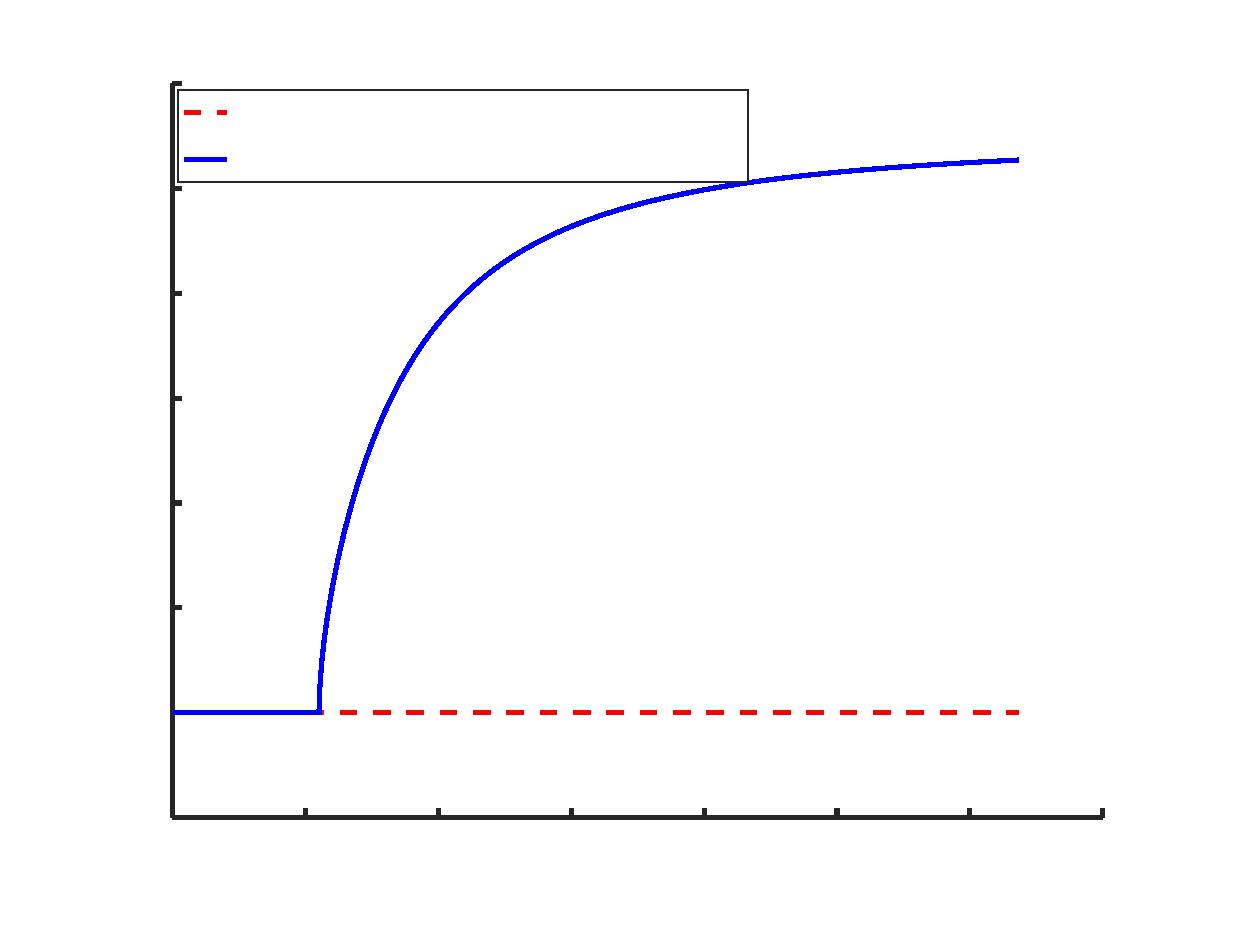
\includegraphics{stabNewmark-inc}
\end{picture}%
\begin{picture}(576,432)(0,0)
\fontsize{16}{0}
\selectfont\put(74.88,42.5189){\makebox(0,0)[t]{\textcolor[rgb]{0.15,0.15,0.15}{{0}}}}
\fontsize{16}{0}
\selectfont\put(138.651,42.5189){\makebox(0,0)[t]{\textcolor[rgb]{0.15,0.15,0.15}{{0.5}}}}
\fontsize{16}{0}
\selectfont\put(202.423,42.5189){\makebox(0,0)[t]{\textcolor[rgb]{0.15,0.15,0.15}{{1}}}}
\fontsize{16}{0}
\selectfont\put(266.194,42.5189){\makebox(0,0)[t]{\textcolor[rgb]{0.15,0.15,0.15}{{1.5}}}}
\fontsize{16}{0}
\selectfont\put(329.966,42.5189){\makebox(0,0)[t]{\textcolor[rgb]{0.15,0.15,0.15}{{2}}}}
\fontsize{16}{0}
\selectfont\put(393.737,42.5189){\makebox(0,0)[t]{\textcolor[rgb]{0.15,0.15,0.15}{{2.5}}}}
\fontsize{16}{0}
\selectfont\put(457.509,42.5189){\makebox(0,0)[t]{\textcolor[rgb]{0.15,0.15,0.15}{{3}}}}
\fontsize{16}{0}
\selectfont\put(521.28,42.5189){\makebox(0,0)[t]{\textcolor[rgb]{0.15,0.15,0.15}{{3.5}}}}
\fontsize{16}{0}
\selectfont\put(69.8755,47.52){\makebox(0,0)[r]{\textcolor[rgb]{0.15,0.15,0.15}{{0.5}}}}
\fontsize{16}{0}
\selectfont\put(69.8755,97.8171){\makebox(0,0)[r]{\textcolor[rgb]{0.15,0.15,0.15}{{1}}}}
\fontsize{16}{0}
\selectfont\put(69.8755,148.114){\makebox(0,0)[r]{\textcolor[rgb]{0.15,0.15,0.15}{{1.5}}}}
\fontsize{16}{0}
\selectfont\put(69.8755,198.411){\makebox(0,0)[r]{\textcolor[rgb]{0.15,0.15,0.15}{{2}}}}
\fontsize{16}{0}
\selectfont\put(69.8755,248.709){\makebox(0,0)[r]{\textcolor[rgb]{0.15,0.15,0.15}{{2.5}}}}
\fontsize{16}{0}
\selectfont\put(69.8755,299.006){\makebox(0,0)[r]{\textcolor[rgb]{0.15,0.15,0.15}{{3}}}}
\fontsize{16}{0}
\selectfont\put(69.8755,349.303){\makebox(0,0)[r]{\textcolor[rgb]{0.15,0.15,0.15}{{3.5}}}}
\fontsize{16}{0}
\selectfont\put(69.8755,399.6){\makebox(0,0)[r]{\textcolor[rgb]{0.15,0.15,0.15}{{4}}}}
\fontsize{16}{0}
\selectfont\put(298.08,23.5189){\makebox(0,0)[t]{\textcolor[rgb]{0.15,0.15,0.15}{{$\Delta t / T$}}}}
\fontsize{16}{0}
\selectfont\put(40.8755,223.56){\rotatebox{90}{\makebox(0,0)[b]{\textcolor[rgb]{0.15,0.15,0.15}{{$\rho(A)$}}}}}
\fontsize{16}{0}
\selectfont\put(103.682,385.714){\makebox(0,0)[l]{\textcolor[rgb]{0,0,0}{{Trapecio: $\alpha=1/4$, $\beta=1/2$}}}}
\fontsize{16}{0}
\selectfont\put(103.682,363.428){\makebox(0,0)[l]{\textcolor[rgb]{0,0,0}{{Acc.Lineal: $\alpha=1/6$, $\beta=1/2$}}}}
\end{picture}
}
	\caption{Estabilidad de variantes del Método de Newmark (Trapecio y Acel. Lineal).}
	\label{fig:stabnewmark}
\end{figure}

Se puede observar que el Método del Trapecio es incondicionalmente estable, mientras que el método de aceleración lineal es condicionalmente estable.

\subsubsection{Ejemplo - Edificio bajo Acción Sísmica}

Finalmente, se presenta un ejemplo en el cual se realiza el análisis dinámico lineal del edificio definido en la Sección~\ref{EjBlast} bajo una acción sísmica. %
%
Para analizar el edificio sometido a movimientos sísmicos laterales de su base, es necesario definir coordenadas absolutas para expresar el movimiento del suelo y otras coordenadas relativas al referencial solidario al suelo.

Los desplazamientos absolutos serán: $\bfu_{G,t}=x_{S,t}\boldsymbol{\iota} + \bfu_{t}$. Donde $\bfu_{G,t}$ son desplazamientos absolutos, $x_{S,t}\boldsymbol{\iota}$ indica la posición del suelo respecto del referencial absoluto y $\bfu_t$ son desplazamientos del edificio relativos al referencial solidario al suelo. Notar que el vector: $\boldsymbol{\iota}$, llamado vector de influencia, indica cómo influye el movimiento de suelo en cada uno de los grados de libertad de la estructura.

Derivando dos veces respecto del tiempo se obtiene: $\ddot{\bfu}_{G,t}=\ddot{x}_{S,t}\boldsymbol{\iota} + \ddot{\bfu}_{t}$. 

Finalmente, notando que las fuerzas internas y los efectos disipativos de la estructura dependen de los desplazamientos relativos $\bfu_t$ y de su derivada primera $\dot{\bfu}_t$, se llega a la ecuación de movimiento bajo acción sísmica:
%
\begin{equation}\label{EcMovLinSismo}
\bfM \ddot{\bfu}_t + \bfC \dot{\bfu}_t + \bfK \bfu_t = -\ddot{x}_{G,t}\bfM \boldsymbol{\iota},
\end{equation}
%
donde $\ddot{x}_{G,t}$ tiene el registro de aceleraciones de suelo medidos según una dirección dada.

En el presente ejemplo, los datos de aceleración corresponden al sismo de Loma Prieta, ocurrido el 17 de octubre de 1987 en California, U.S.A. %\footnote{Obtenidos de \url{http://peer.berkeley.edu/products/strong_ground_motion_db.html}} 

En la Figura~\ref{fig:LomaPrieta} se muestran los resultados de la solución de la dinámica del edificio para la aceleración de terreno elegida. %
Comparando los resultados obtenidos con los de la solución de la dinámica del edificio sometido a una detonación, se observa mayores desplazamientos en el caso del sismo.

\begin{figure}[htb]
	\centering
	\resizebox{.95\linewidth}{!}{% Title: gl2ps_renderer figure
% Creator: GL2PS 1.4.0, (C) 1999-2017 C. Geuzaine
% For: Octave
% CreationDate: Fri Dec 29 11:53:58 2017
\setlength{\unitlength}{1pt}
\begin{picture}(0,0)
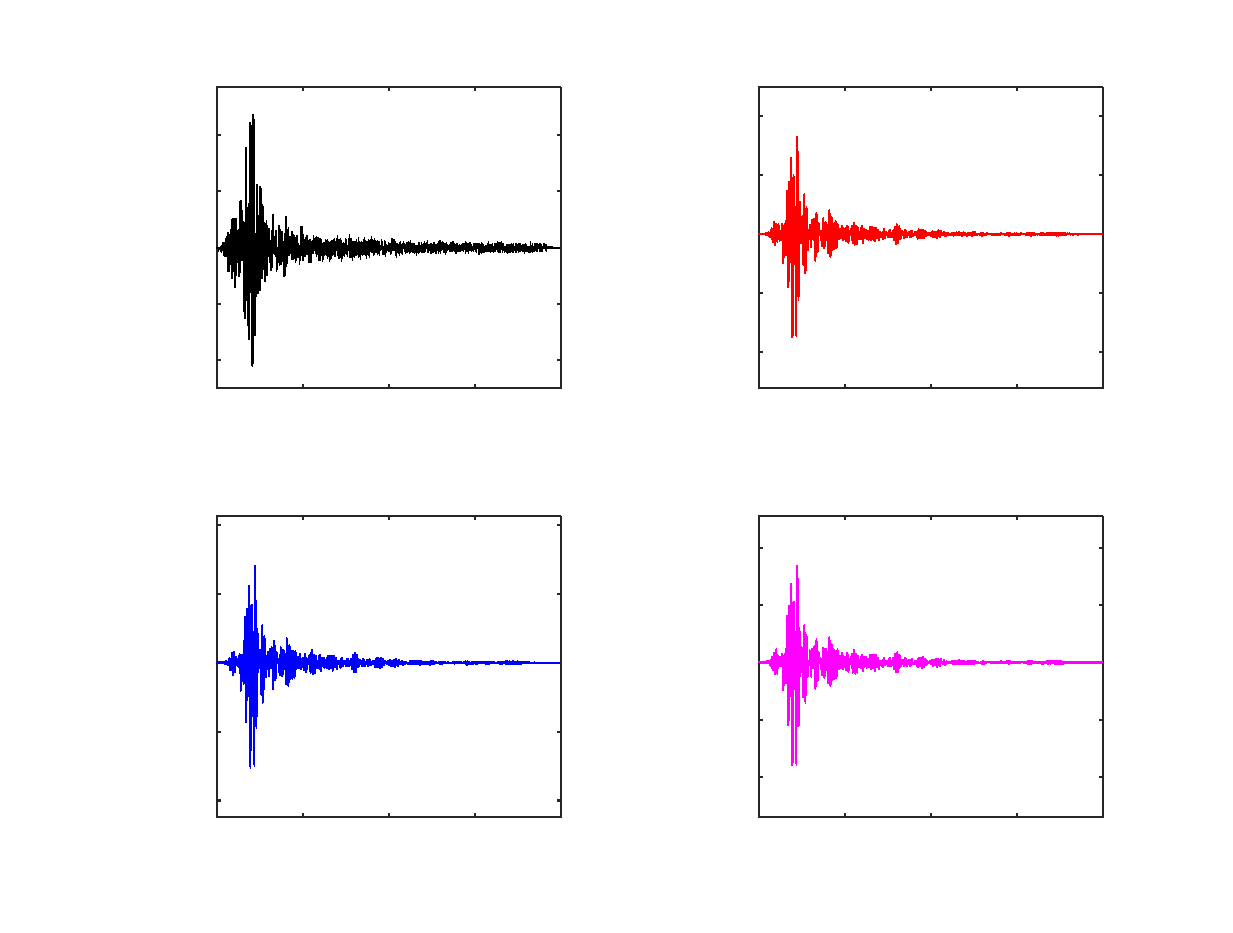
\includegraphics{sismo-inc}
\end{picture}%
\begin{picture}(576,432)(0,0)
\fontsize{15}{0}
\selectfont\put(356.265,248.393){\makebox(0,0)[t]{\textcolor[rgb]{0.15,0.15,0.15}{{0}}}}
\fontsize{15}{0}
\selectfont\put(397.519,248.393){\makebox(0,0)[t]{\textcolor[rgb]{0.15,0.15,0.15}{{10}}}}
\fontsize{15}{0}
\selectfont\put(438.773,248.393){\makebox(0,0)[t]{\textcolor[rgb]{0.15,0.15,0.15}{{20}}}}
\fontsize{15}{0}
\selectfont\put(480.026,248.393){\makebox(0,0)[t]{\textcolor[rgb]{0.15,0.15,0.15}{{30}}}}
\fontsize{15}{0}
\selectfont\put(521.28,248.393){\makebox(0,0)[t]{\textcolor[rgb]{0.15,0.15,0.15}{{40}}}}
\fontsize{15}{0}
\selectfont\put(351.265,270.871){\makebox(0,0)[r]{\textcolor[rgb]{0.15,0.15,0.15}{{-0.01}}}}
\fontsize{15}{0}
\selectfont\put(351.265,299.164){\makebox(0,0)[r]{\textcolor[rgb]{0.15,0.15,0.15}{{-0.005}}}}
\fontsize{15}{0}
\selectfont\put(351.265,327.457){\makebox(0,0)[r]{\textcolor[rgb]{0.15,0.15,0.15}{{0}}}}
\fontsize{15}{0}
\selectfont\put(351.265,355.75){\makebox(0,0)[r]{\textcolor[rgb]{0.15,0.15,0.15}{{0.005}}}}
\fontsize{15}{0}
\selectfont\put(351.265,384.042){\makebox(0,0)[r]{\textcolor[rgb]{0.15,0.15,0.15}{{0.01}}}}
\fontsize{15}{0}
\selectfont\put(438.773,230.393){\makebox(0,0)[t]{\textcolor[rgb]{0.15,0.15,0.15}{{t [s]}}}}
\fontsize{15}{0}
\selectfont\put(297.265,325.629){\rotatebox{90}{\makebox(0,0)[b]{\textcolor[rgb]{0.15,0.15,0.15}{{$u_1(t)$ [m]}}}}}
\fontsize{15}{0}
\selectfont\put(96.036,42.5047){\makebox(0,0)[t]{\textcolor[rgb]{0.15,0.15,0.15}{{0}}}}
\fontsize{15}{0}
\selectfont\put(137.29,42.5047){\makebox(0,0)[t]{\textcolor[rgb]{0.15,0.15,0.15}{{10}}}}
\fontsize{15}{0}
\selectfont\put(178.543,42.5047){\makebox(0,0)[t]{\textcolor[rgb]{0.15,0.15,0.15}{{20}}}}
\fontsize{15}{0}
\selectfont\put(219.797,42.5047){\makebox(0,0)[t]{\textcolor[rgb]{0.15,0.15,0.15}{{30}}}}
\fontsize{15}{0}
\selectfont\put(261.051,42.5047){\makebox(0,0)[t]{\textcolor[rgb]{0.15,0.15,0.15}{{40}}}}
\fontsize{15}{0}
\selectfont\put(91.0356,55.6037){\makebox(0,0)[r]{\textcolor[rgb]{0.15,0.15,0.15}{{-0.02}}}}
\fontsize{15}{0}
\selectfont\put(91.0356,88.6513){\makebox(0,0)[r]{\textcolor[rgb]{0.15,0.15,0.15}{{-0.01}}}}
\fontsize{15}{0}
\selectfont\put(91.0356,121.699){\makebox(0,0)[r]{\textcolor[rgb]{0.15,0.15,0.15}{{0}}}}
\fontsize{15}{0}
\selectfont\put(91.0356,154.747){\makebox(0,0)[r]{\textcolor[rgb]{0.15,0.15,0.15}{{0.01}}}}
\fontsize{15}{0}
\selectfont\put(91.0356,187.794){\makebox(0,0)[r]{\textcolor[rgb]{0.15,0.15,0.15}{{0.02}}}}
\fontsize{15}{0}
\selectfont\put(178.543,24.5047){\makebox(0,0)[t]{\textcolor[rgb]{0.15,0.15,0.15}{{t [s]}}}}
\fontsize{15}{0}
\selectfont\put(47.0355,119.74){\rotatebox{90}{\makebox(0,0)[b]{\textcolor[rgb]{0.15,0.15,0.15}{{$u_2(t)$ [m]}}}}}
\fontsize{15}{0}
\selectfont\put(356.265,42.5047){\makebox(0,0)[t]{\textcolor[rgb]{0.15,0.15,0.15}{{0}}}}
\fontsize{15}{0}
\selectfont\put(397.519,42.5047){\makebox(0,0)[t]{\textcolor[rgb]{0.15,0.15,0.15}{{10}}}}
\fontsize{15}{0}
\selectfont\put(438.773,42.5047){\makebox(0,0)[t]{\textcolor[rgb]{0.15,0.15,0.15}{{20}}}}
\fontsize{15}{0}
\selectfont\put(480.026,42.5047){\makebox(0,0)[t]{\textcolor[rgb]{0.15,0.15,0.15}{{30}}}}
\fontsize{15}{0}
\selectfont\put(521.28,42.5047){\makebox(0,0)[t]{\textcolor[rgb]{0.15,0.15,0.15}{{40}}}}
\fontsize{15}{0}
\selectfont\put(351.265,66.824){\makebox(0,0)[r]{\textcolor[rgb]{0.15,0.15,0.15}{{-0.02}}}}
\fontsize{15}{0}
\selectfont\put(351.265,94.3379){\makebox(0,0)[r]{\textcolor[rgb]{0.15,0.15,0.15}{{-0.01}}}}
\fontsize{15}{0}
\selectfont\put(351.265,121.852){\makebox(0,0)[r]{\textcolor[rgb]{0.15,0.15,0.15}{{0}}}}
\fontsize{15}{0}
\selectfont\put(351.265,149.366){\makebox(0,0)[r]{\textcolor[rgb]{0.15,0.15,0.15}{{0.01}}}}
\fontsize{15}{0}
\selectfont\put(351.265,176.88){\makebox(0,0)[r]{\textcolor[rgb]{0.15,0.15,0.15}{{0.02}}}}
\fontsize{15}{0}
\selectfont\put(438.773,24.5047){\makebox(0,0)[t]{\textcolor[rgb]{0.15,0.15,0.15}{{t [s]}}}}
\fontsize{15}{0}
\selectfont\put(307.265,119.74){\rotatebox{90}{\makebox(0,0)[b]{\textcolor[rgb]{0.15,0.15,0.15}{{$u_3(t)$ [m]}}}}}
\fontsize{15}{0}
\selectfont\put(96.036,248.393){\makebox(0,0)[t]{\textcolor[rgb]{0.15,0.15,0.15}{{0}}}}
\fontsize{15}{0}
\selectfont\put(137.29,248.393){\makebox(0,0)[t]{\textcolor[rgb]{0.15,0.15,0.15}{{10}}}}
\fontsize{15}{0}
\selectfont\put(178.543,248.393){\makebox(0,0)[t]{\textcolor[rgb]{0.15,0.15,0.15}{{20}}}}
\fontsize{15}{0}
\selectfont\put(219.797,248.393){\makebox(0,0)[t]{\textcolor[rgb]{0.15,0.15,0.15}{{30}}}}
\fontsize{15}{0}
\selectfont\put(261.051,248.393){\makebox(0,0)[t]{\textcolor[rgb]{0.15,0.15,0.15}{{40}}}}
\fontsize{15}{0}
\selectfont\put(91.0356,266.84){\makebox(0,0)[r]{\textcolor[rgb]{0.15,0.15,0.15}{{-0.4}}}}
\fontsize{15}{0}
\selectfont\put(91.0356,293.919){\makebox(0,0)[r]{\textcolor[rgb]{0.15,0.15,0.15}{{-0.2}}}}
\fontsize{15}{0}
\selectfont\put(91.0356,320.998){\makebox(0,0)[r]{\textcolor[rgb]{0.15,0.15,0.15}{{0}}}}
\fontsize{15}{0}
\selectfont\put(91.0356,348.077){\makebox(0,0)[r]{\textcolor[rgb]{0.15,0.15,0.15}{{0.2}}}}
\fontsize{15}{0}
\selectfont\put(91.0356,375.156){\makebox(0,0)[r]{\textcolor[rgb]{0.15,0.15,0.15}{{0.4}}}}
\fontsize{15}{0}
\selectfont\put(178.543,230.393){\makebox(0,0)[t]{\textcolor[rgb]{0.15,0.15,0.15}{{t [s]}}}}
\fontsize{15}{0}
\selectfont\put(57.0355,325.629){\rotatebox{90}{\makebox(0,0)[b]{\textcolor[rgb]{0.15,0.15,0.15}{{accel [g]}}}}}
\fontsize{11}{0}
\selectfont\put(178.543,407.849){\makebox(0,0)[b]{\textcolor[rgb]{0,0,0}{{Aceleracion del Terreno por Sismo}}}}
\end{picture}
}
	\caption{Solución numérica del movimiento del edificio bajo acción de sismo.}
	\label{fig:LomaPrieta}
\end{figure}


\section{Dinámica No Lineal}\label{DinNoLin}

Luego de haber estudiado los procedimientos de solución de la ecuación de movimiento para una estructura sin considerar no linealidades, se puede pasar a estudiar los cambios necesarios para poder resolver la dinámica considerando no linealidades, es decir Dinámica No Lineal.

Tal como fue presentada en la Sección \ref{EcMov}, la ecuación de movimiento para una estructura no lineal tiene un vector de fuerzas internas que es función de $\bfu_t$. Dicho vector puede contemplar no linealidad material, geométrica o de ambos tipos.
%
\begin{equation}
\bfM \ddot{\bfu}_t + \bfC \dot{\bfu}_t + \bff_{\text{int}}(\bfu_t) = \bff_{\text{ext},t}
\end{equation}

Los procedimientos de solución explícitos e implícitos se deben ajustar al hecho de que el vector de fuerzas internas ya no es simplemente el producto de la matriz de rigidez por el vector de desplazamientos en el tiempo considerado. %
%
Este cambio tiene un efecto menor en el procedimiento correspondiente al Método de Diferencia Centrada, pero implica un cambio significativo en el procedimiento asociado al Método de Newmark.

De manera resumida, en el caso de dinámica no lineal, se deberá asegurar que el equilibrio se verifica para cada instante de tiempo. En el caso de métodos explícitos eso es inmediato, pero en el caso de métodos implícitos esto requerirá de iteraciones de tipo N-R para asegurar dicho equilibrio.

También cabe mencionar que los criterios de estabilidad numérica vistos para el caso de estructuras lineales no aplican de manera inmediata al caso no lineal. En particular, siempre y cuando el paso temporal ($\Delta t$) sea suficientemente corto, tal que la estructura mantenga un comportamiento aproximadamente lineal durante varios instantes de tiempo, los criterios de estabilidad tendrán cierto grado de validez. Se debe tomar en cuenta que los períodos de vibración relevantes para determinar la estabilidad numérica corresponden a la rigidez de la estructura a medida que transcurre el tiempo. Una estructura que se vuelve más rígida por efectos geométricos a medida que avanza el tiempo, tendrá, para el Método de Diferencia Centrada, un paso temporal crítico cada vez menor debido a dicho aumento de la rigidez.

Para pasos temporales largos, tales que de un instante a otro el comportamiento de la estructura no puede considerarse aproximadamente lineal, los criterios de estabilidad no aplican y se pueden llegar a observar inestabilidades numéricas en métodos que se clasificaron como incondicionalmente estables para problemas lineales.

\subsection{Método de Diferencia Centrada - Explícito}

La deducción del método es idéntica a la presentada en la sección de dinámica lineal. Se busca determinar $\bfu_{t+\Delta t}$, para ello se considera el equilibrio dinámico en el tiempo $t$ y se usan los mismos cocientes incrementales para aproximar las derivadas primera y segunda de $\bfu_t$. En este caso se debe simplemente tomar en cuenta que las fuerzas internas están dadas por $\bff_{\text{int}}(\bfu_{t})$.

Usando la Ecuación~\eqref{EcDifCent} se puede escribir,
%
\begin{equation}\label{EcDifCentNL}
\begin{split}
\left[\frac{1}{\Delta t^2}\bfM + \frac{1}{2\Delta t}\bfC \right] \bfu_{t+\Delta t} = \bff_{ext,t} - &\bff_{\text{int}}(\bfu_{t}) + \frac{2}{\Delta t ^2}\bfM \bfu_t \\
- & \left[\frac{1}{\Delta t^2}\bfM-\frac{1}{2\Delta t}\bfC\right] \bfu_{t-\Delta t}.
\end{split}
\end{equation}

La Ecuación~\eqref{EcDifCentNL} provee la regla mediante la cual se calcula $\bfu_{t+\Delta t}$. Notar que en el caso de una estructura no lineal debemos en cada paso evaluar el vector de fuerzas internas en el instante de tiempo actual. Es claro que el método continúa siendo explícito. 

Se destaca que sigue siendo necesario, tal como en la solución de problemas lineales, que la matriz de masa y eventualmente la de amortiguamiento sean diagonales de manera que la evaluación de $\bfu_{t+\Delta t}$ a partir de la Ecuación~\eqref{EcDifCentNL} sea computacionalmente económica.

A partir del desarrollo anterior, se puede actualizar el procedimiento de solución del Método de Diferencia Centrada para el caso de estructuras no lineales tal como se muestra en el Algoritmo~\ref{PCDifCentNL}.

\begin{algorithm}
	
	\caption{Método de Diferencia Centrada - No-Lineal}
	\label{PCDifCentNL}
	
	\begin{algorithmic}[1]
		
		\STATE Ensamblar: $\bfM$ y $\bfC$ a nivel de estructura.
		\STATE Definir: tiempo final de análisis dinámico: $t_f$
		\STATE Definir: Condiciones iniciales: $\bfu_{0}$, $\dot{\bfu}_{0}$
		\STATE Calcular: $\ddot{\bfu}_{0}\leftarrow \bfM^{-1}(\bff_{ext,t} - \bfC \dot{\bfu}_0 - \bff_{\text{int}}(\bfu_0))$
		\STATE Definir: $\Delta t$, considerar estabilidad numérica.
		\STATE Calcular: $a_0\leftarrow1/\Delta t^2$, $a_1\leftarrow1/(2\Delta t)$, $a_2\leftarrow2a_0$ y $a_3\leftarrow1/a_2$
		\STATE Calcular: $\bfu_{-\Delta t} \leftarrow \bfu_0 - \Delta t \dot{\bfu}_0 + a_3\ddot{\bfu}_0$
		\STATE Calcular y factorizar: $\hat{\bfM}\leftarrow a_0\bfM+a_1\bfC$
		\STATE $t \leftarrow 0$
		\WHILE{$t<t_f$}
		\STATE Calcular: $\hat{\bff}_t\leftarrow \bff_{ext,t} -\bff_{\text{int}}(\bfu_t) +a_2\bfM \bfu_t - (a_0\bfM-a_1\bfC)\bfu_{t-\Delta t}$
		\STATE Resolver: $\bfu_{t+\Delta t}\leftarrow \hat{\bfM}^{-1}\hat{\bff}_t$
		\STATE Calcular aceleración: $\ddot{\bfu}_{t}\leftarrow a_0(\bfu_{t+\Delta t}-2\bfu_{t}+\bfu_{t-\Delta t})$
		\STATE Calcular velocidad: $\dot{\bfu}_{t}\leftarrow a_1(\bfu_{t+\Delta t}-\bfu_{t-\Delta t})$
		\STATE $t\leftarrow t+\Delta t$
		\ENDWHILE
		
	\end{algorithmic}
	
\end{algorithm}

En este momento es una buena idea comentar sobre la elección del paso temporal ($\Delta t$) para el Método de Diferencia Centrada en problemas no lineales. Tal como se mencionó anteriormente, la estabilidad numérica del método continúa restringiendo el paso temporal máximo que se puede usar. La elección del paso se vuelve más difícil en el caso de estructuras no lineales ya que el paso temporal crítico no es constante durante la solución. %
%
La rigidez de la estructura puede variar a lo largo del tiempo por efectos de rigidez geométrica o por no linealidad material. Si se espera que la estructura solamente se flexibilice a medida que transcurre el tiempo, un criterio razonable puede ser determinar el paso temporal en base a la rigidez inicial de la estructura. Si este no es el caso, se debe prever el efecto de la rigidización de la estructura en el paso temporal crítico y asegurar que el paso elegido no superará el valor crítico mínimo previsto.

Al realizar análisis dinámicos de estructuras no lineales usando el Método de Diferencia centrada, la elección de un paso temporal demasiado largo en comparación con el mínimo paso temporal crítico previsto, puede llevar a acumular errores significativos durante aquellos instantes de tiempo en los cuales el paso temporal elegido superó al paso crítico. %
%
Esta acumulación acotada de errores es marcadamente distinta a la que se observa en análisis dinámicos lineales, en los cuales si se elije un paso temporal por encima del valor crítico, la solución diverge y el analista puede reconocer fácilmente que seleccionó un paso temporal erróneo.


\subsubsection{Ejemplo Dinámica No Lineal - Cercha de Von Mises}

Se considera una cercha de tipo de Von Mises bajo la acción de una carga dinámica. %
%
La estructura consiste en dos columnas flexibles empotradas en la base y dos bielas articuladas que trabajan como puntales de la cercha tal como se muestra en la Figura~\ref{fig:GeomVM}. %

Se coloca una masa $m$ suspendida de la cumbre de la cercha. %
%
Todas las barras de la cercha están formada por acero ($E=200 \text{ GPa}$) y sección rectangular ($a=3.2\text{mm}$ y $b=25.4\text{mm}$). %
%
Los parámetros que definen la geometría son: $L_c = 240 $ mm, $L_x= 187$ mm y $L_z=84$ mm. %
%
Esta estructura es la utilizada por el profesor A. Wadee en la presentación referida al inicio del Capítulo 2 de este documento.

\begin{figure}[htb]
	\centering
	\def\svgwidth{0.7\textwidth}
\input{../fig/misses_truss_Cap4.pdf_tex}
	\caption{Geometría de Cercha de Von Mises.}
	\label{fig:GeomVM}
\end{figure}

La forma de cargar la estructura consiste en suspender la masa en la configuración indeformada y luego dejarla libre. Esto implica que el vector de deformación inicial es nulo y también lo es el vector de velocidades inicial.

Dada la simetría axial, respecto al eje vertical, presente en la estructura y las cargas aplicadas, se modela la mitad izquierda de la estructura. %
%
De esta forma solo se debe analizar una biela de Green con condición de borde deslizante vertical en el extremo derecho y deslizante horizontal con resorte en el extremo izquierdo tal como se muestra en la Figura~\ref{fig:ModelVM}. %
%
La constante elástica del resorte está dado por la rigidez flexional de los pilares.

\begin{figure}[htb]
	\centering
	\def\svgwidth{0.6\textwidth}
\input{../fig/misses_truss_Cap4_simetr.pdf_tex}
	\caption{Modelo de Cálculo de Cercha de Von Mises.}
	\label{fig:ModelVM}
\end{figure}

El vector de desplazamientos es considerado $\bfu_t = (u_{1,t}, u_{2,t})^\text{T}$ y por lo tanto la ecuación dinámica está dada por:
%
\begin{equation}
\bfM \ddot{\bfu}_t + \bfC \dot{\bfu}_t + \bff_{\text{int}}(\bfu_t)=\bff_{ext,t}.
\end{equation}	
%
Dado que se está analizando media estructura la matriz de masa es igual a:
%
$$\bfM = \left[\begin{array}{cc}m_b& 0\\ 0& (m_b+m)/2\end{array}\right],$$
%
donde $m_b$ es la masa de una biela o columna y $m$ es la masa suspendida del centro de la cercha. Dicha masa se considera rígidamente vinculada a la cercha en la dirección vertical.

Se considera que existe amortiguamiento, para lo cual se introduce una constante $c$ empírica de amortiguamiento de manera de reproducir un amortiguamiento realista de la estructura. %
%
Se usa $c$ para el grado de libertad de movimiento vertical y $c/10$ para el de movimiento horizontal, por lo que la matriz $\bfC$ está dada por:
$$\bfC = \left[\begin{array}{cc}c/10& 0\\ 0& c\end{array}\right].$$
%
A través de estos amortiguamientos se pretende introducir el arrastre de la pesa debido al aire y la fricción existente en las bisagras que forman las articulaciones de la cercha en el modelo.

Para resolver la dinámica de esta estructura se aplica el Método de Diferencia Centrada, el cual requiere que el usuario calcule únicamente el vector de fuerzas internas. %
%
En lo que sigue se deducirá $\bff_{\text{int}}(\bfu_t)$ asumiendo que las bielas son de tipo Green y que la columna se puede modelar como un resorte lineal horizontal de constante $k_c$,  donde $k_c$ está dado por la rigidez flexional $3 E I_c / L_c^3$.

El vector de fuerzas internas de la biela se deduce usando el PTV. Evaluando el trabajo virtual interno se tiene:
%
\begin{equation}
\delta W_{\text{int}}=\delta\bfu^T \bff_{\text{int}}(\bfu_t)= \int_{l_0} \sigma_t \delta\varepsilon_G A dx + \delta\bfu^T\bfK_s \bfu_t,
\end{equation}
%
donde el segundo sumando del trabajo virtual interno corresponde al trabajo virtual interno de la fuerza realizada por el resorte horizontal de constante $k_c$.

La deformación unitaria de Green para la biela está dada por:
%
\begin{equation}
\varepsilon_G = \frac{l_t^2 - l_0^2}{2 l_0^2}.
\end{equation}

Se asume una relación constitutiva elástica lineal entre tensión y deformación de Green, válido para pequeñas deformaciones unitarias pero grandes desplazamientos y rotaciones.
%
\begin{equation}
\sigma = E \varepsilon_G.
\end{equation}

Los largos de barra iniciales (de referencia) y actuales (deformada) se pueden escribir como:
%
\begin{equation}
l_0 ^2 = L_x^2+ L_z^2 \quad \text{y} \quad 
l_t ^2 = (L_x-u_{1,t})^2+ (L_z+u_{2,t})^2,
\end{equation}
respectivamente, con lo cual la deformación de Green se reduce a:
%
\begin{equation}
\varepsilon_G = \frac{-2 L_x u_{1,t}+2 L_z u_{2,t} + u_{1,t}^2 + u_{2,t}^2}{2 (L_x^2+L_z^2)}.
\end{equation}

Se procede a calcular la variación de la deformación de Green ($\delta \varepsilon_G$):
%
\begin{eqnarray}
	\delta \varepsilon_G &=& \dfrac{1}{L_x^2+L_z^2}\left[ (-L_x + u_1)\delta u_1 + (L_z+u_2)\delta u_2 \right] \\
	 &=& \delta\bfu^T  \left[\begin{array}{c} -L_x + u_{1,t}\\ L_z + u_{2,t}\end{array}\right] \dfrac{1}{l_0^2},
\end{eqnarray}
con lo cual, el vector de fuerzas internas para la barra de Green y el resorte lineal resulta:
%
\begin{equation}
\begin{split}
	\bff_{\text{int}}(\bfu_t) = \dfrac{E A l_0(u_{1,t}^2 + u_{2,t}^2 -2 L_x u_{1,t}+2 L_z u_{2,t})}{2 l_0^4} &\left[\begin{array}{c} -L_x + u_{1,t}\\ L_z + u_{2,t}\end{array}\right] \\ +& \left[\begin{array}{c} k_c u_{1,t}\\ 0\end{array}\right].
\end{split}
\end{equation}

Finalmente, la fuerza externa dinámica aplicada sobre la cercha resulta en un vector $\bff_{\text{ext},t}$ dado por:
%
\begin{equation}
\bff_{\text{ext},t} = \left[\begin{array}{c} 0\\ -g(m_b+m)/2\end{array}\right].
\end{equation}

\textbf{Solución Numérica - Método de Diferencia Centrada:}

Para obtener la solución numérica se debe definir un paso temporal $\Delta t$ tal que el método de Diferencia Centrada sea estable.

\cajaactividad{
Discutir y estimar cuánto vale $\Delta T_{cr}$ para el ejemplo de la cercha de Von Mises.
}

Luego de definido $\Delta T_{cr}$ se procede a implementar el método. En el Código~\ref{cod:VonMisesCod} se muestra una implementación para la resolución del ejemplo.

\lstinputlisting[caption = {Código para análisis dinámico de cercha de Von Mises.}\label{cod:VonMisesCod}]{../src/VonMisesNL_DifCent.m}

En la Figura~\ref{fig:ResVM} se muestra la solución de la dinámica para una masa suspendida igual a $m = 1.4$ kg.

\begin{figure}[!htb]
	\centering
	\resizebox{.95\linewidth}{!}{% Title: gl2ps_renderer figure
% Creator: GL2PS 1.4.0, (C) 1999-2017 C. Geuzaine
% For: Octave
% CreationDate: Fri Dec 29 11:58:15 2017
\setlength{\unitlength}{1pt}
\begin{picture}(0,0)
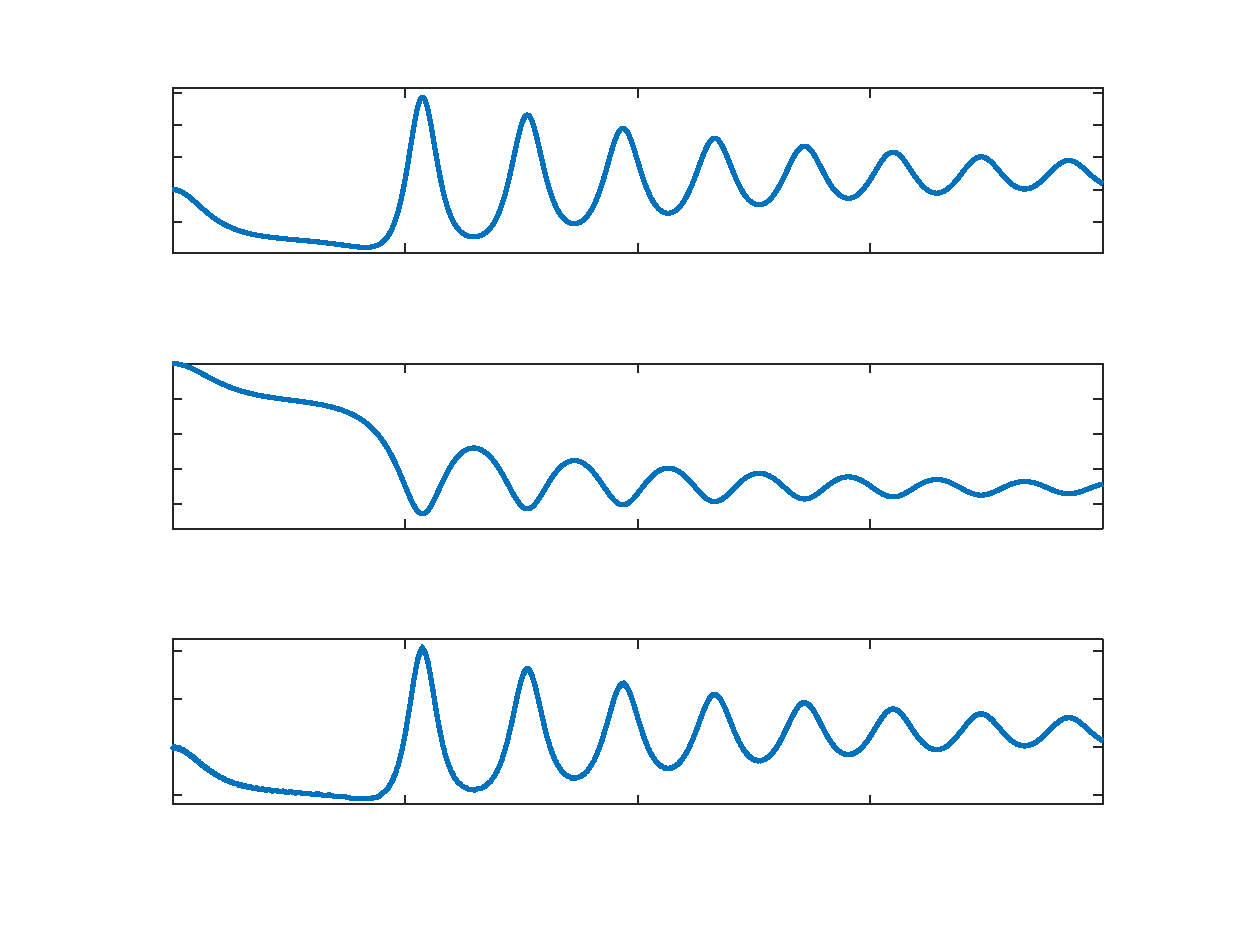
\includegraphics{PlotsVMises-inc}
\end{picture}%
\begin{picture}(576,432)(0,0)
\fontsize{16}{0}
\selectfont\put(74.88,313.318){\makebox(0,0)[t]{\textcolor[rgb]{0.15,0.15,0.15}{{0}}}}
\fontsize{16}{0}
\selectfont\put(186.48,313.318){\makebox(0,0)[t]{\textcolor[rgb]{0.15,0.15,0.15}{{0.5}}}}
\fontsize{16}{0}
\selectfont\put(298.08,313.318){\makebox(0,0)[t]{\textcolor[rgb]{0.15,0.15,0.15}{{1}}}}
\fontsize{16}{0}
\selectfont\put(409.68,313.318){\makebox(0,0)[t]{\textcolor[rgb]{0.15,0.15,0.15}{{1.5}}}}
\fontsize{16}{0}
\selectfont\put(521.28,313.318){\makebox(0,0)[t]{\textcolor[rgb]{0.15,0.15,0.15}{{2}}}}
\fontsize{16}{0}
\selectfont\put(69.8755,333.446){\makebox(0,0)[r]{\textcolor[rgb]{0.15,0.15,0.15}{{-10}}}}
\fontsize{16}{0}
\selectfont\put(69.8755,348.867){\makebox(0,0)[r]{\textcolor[rgb]{0.15,0.15,0.15}{{0}}}}
\fontsize{16}{0}
\selectfont\put(69.8755,364.287){\makebox(0,0)[r]{\textcolor[rgb]{0.15,0.15,0.15}{{10}}}}
\fontsize{16}{0}
\selectfont\put(69.8755,379.707){\makebox(0,0)[r]{\textcolor[rgb]{0.15,0.15,0.15}{{20}}}}
\fontsize{16}{0}
\selectfont\put(69.8755,395.128){\makebox(0,0)[r]{\textcolor[rgb]{0.15,0.15,0.15}{{30}}}}
\fontsize{16}{0}
\selectfont\put(298.08,294.318){\makebox(0,0)[t]{\textcolor[rgb]{0.15,0.15,0.15}{{$t$ [s]}}}}
\fontsize{16}{0}
\selectfont\put(39.8755,357.968){\rotatebox{90}{\makebox(0,0)[b]{\textcolor[rgb]{0.15,0.15,0.15}{{$u_1$ [mm]}}}}}
\fontsize{16}{0}
\selectfont\put(74.88,181.025){\makebox(0,0)[t]{\textcolor[rgb]{0.15,0.15,0.15}{{0}}}}
\fontsize{16}{0}
\selectfont\put(186.48,181.025){\makebox(0,0)[t]{\textcolor[rgb]{0.15,0.15,0.15}{{0.5}}}}
\fontsize{16}{0}
\selectfont\put(298.08,181.025){\makebox(0,0)[t]{\textcolor[rgb]{0.15,0.15,0.15}{{1}}}}
\fontsize{16}{0}
\selectfont\put(409.68,181.025){\makebox(0,0)[t]{\textcolor[rgb]{0.15,0.15,0.15}{{1.5}}}}
\fontsize{16}{0}
\selectfont\put(521.28,181.025){\makebox(0,0)[t]{\textcolor[rgb]{0.15,0.15,0.15}{{2}}}}
\fontsize{16}{0}
\selectfont\put(69.8755,198.054){\makebox(0,0)[r]{\textcolor[rgb]{0.15,0.15,0.15}{{-200}}}}
\fontsize{16}{0}
\selectfont\put(69.8755,214.867){\makebox(0,0)[r]{\textcolor[rgb]{0.15,0.15,0.15}{{-150}}}}
\fontsize{16}{0}
\selectfont\put(69.8755,231.68){\makebox(0,0)[r]{\textcolor[rgb]{0.15,0.15,0.15}{{-100}}}}
\fontsize{16}{0}
\selectfont\put(69.8755,248.494){\makebox(0,0)[r]{\textcolor[rgb]{0.15,0.15,0.15}{{-50}}}}
\fontsize{16}{0}
\selectfont\put(69.8755,265.307){\makebox(0,0)[r]{\textcolor[rgb]{0.15,0.15,0.15}{{0}}}}
\fontsize{16}{0}
\selectfont\put(298.08,162.025){\makebox(0,0)[t]{\textcolor[rgb]{0.15,0.15,0.15}{{$t$ [s]}}}}
\fontsize{16}{0}
\selectfont\put(29.8755,225.674){\rotatebox{90}{\makebox(0,0)[b]{\textcolor[rgb]{0.15,0.15,0.15}{{$u_2$ [mm]}}}}}
\fontsize{16}{0}
\selectfont\put(74.88,48.731){\makebox(0,0)[t]{\textcolor[rgb]{0.15,0.15,0.15}{{0}}}}
\fontsize{16}{0}
\selectfont\put(186.48,48.731){\makebox(0,0)[t]{\textcolor[rgb]{0.15,0.15,0.15}{{0.5}}}}
\fontsize{16}{0}
\selectfont\put(298.08,48.731){\makebox(0,0)[t]{\textcolor[rgb]{0.15,0.15,0.15}{{1}}}}
\fontsize{16}{0}
\selectfont\put(409.68,48.731){\makebox(0,0)[t]{\textcolor[rgb]{0.15,0.15,0.15}{{1.5}}}}
\fontsize{16}{0}
\selectfont\put(521.28,48.731){\makebox(0,0)[t]{\textcolor[rgb]{0.15,0.15,0.15}{{2}}}}
\fontsize{16}{0}
\selectfont\put(69.8755,58.3215){\makebox(0,0)[r]{\textcolor[rgb]{0.15,0.15,0.15}{{-50}}}}
\fontsize{16}{0}
\selectfont\put(69.8755,81.347){\makebox(0,0)[r]{\textcolor[rgb]{0.15,0.15,0.15}{{0}}}}
\fontsize{16}{0}
\selectfont\put(69.8755,104.373){\makebox(0,0)[r]{\textcolor[rgb]{0.15,0.15,0.15}{{50}}}}
\fontsize{16}{0}
\selectfont\put(69.8755,127.398){\makebox(0,0)[r]{\textcolor[rgb]{0.15,0.15,0.15}{{100}}}}
\fontsize{16}{0}
\selectfont\put(298.08,29.731){\makebox(0,0)[t]{\textcolor[rgb]{0.15,0.15,0.15}{{$t$ [s]}}}}
\fontsize{16}{0}
\selectfont\put(35.8755,93.3804){\rotatebox{90}{\makebox(0,0)[b]{\textcolor[rgb]{0.15,0.15,0.15}{{Directa [N]}}}}}
\end{picture}
}
	\caption{Resultados de Cercha de Von Mises (m=1.4kg) - Dinámica}
	\label{fig:ResVM}
\end{figure}


Para valores de masa mayores a $1.4$ kg se observa pandeo tipo \textit{Snap-through} dinámico de la estructura.

\cajaactividad{
Compare este valor con el valor de carga crítica correspondiente a carga cuasi-estática.
}


\subsection{Método de Newmark - Implícito}

La deducción de este método es similar a la presentada en la sección de dinámica lineal. %
%
El objetivo es determinar $\bfu_{t+\Delta t}$, para ello Newmark considera el equilibrio dinámico en el tiempo $t+\Delta t$ y se usan las mismas expresiones de tipo Taylor para aproximar $\bfu_{t+\Delta t}$ y $\dot{\bfu}_{t+\Delta t}$. Se debe notar que las fuerzas internas en el tiempo $t+\Delta t$ están dadas por $\bff_{\text{int}}(\bfu_{t+\Delta t})$.

Lo anterior, en conjunto con las Ecuaciones \eqref{Newmark1} y \eqref{Newmark2}, permiten obtener la expresión:
%
\begin{equation}\label{NewmarkNL1}
\bff_{\text{int}}(\bfu_{t+\Delta t})+\left[ \frac{1}{\alpha \Delta t^2} \bfM + \frac{\delta}{\alpha \Delta t} \bfC \right] \bfu_{t+\Delta t} = \hat{\bff}_{t+\Delta t},
\end{equation}
%
donde la definición de $\hat{\bff}_{t+\Delta t}$ es la misma que la dada en la Sección~\ref{FormNewmarkLin}. %

Se observa por lo tanto que para determinar $\bfu_{t+\Delta t}$ mediante Newmark, para el caso de un problema dinámico no lineal, se debe resolver la ecuación no lineal dada por la Ecuación~\eqref{NewmarkNL1}. %
%
Esto es claramente más laborioso que en el caso de un problema dinámico lineal, en el cual cada paso de Newmark consistía simplemente en resolver un sistema de ecuaciones lineales.

\cajaactividad{
Formular la solución de la ecuación no lineal definida en el paso de Newmark aplicando soluciones iterativas de tipo Newton-Raphson o incluso Newton-Raphson modificado.
}

Para los métodos de tipo Newton-Raphson se debe usar la matriz tangente $\bfK_T = \partial \bff_{\text{int}} / \partial \bfu$, que ya fue presentada en el caso de análisis estáticos. %
%
Para que la solución sea correcta se debe iterar hasta obtener convergencia del equilibrio dinámico en el paso $t+\Delta t$, con lo cual los criterios de convergencia son similares a los ya discutidos anteriormente, aunque usando la ecuación no lineal dada en esta sección.

Tal como se indicó al comienzo de esta sección, si el paso temporal es suficientemente corto como para que la estructura se comporte de forma aproximadamente lineal durante varios instantes de tiempo, entonces Newmark presentará un comportamiento estable. A pesar de esto, es posible seleccionar pasos temporales suficientemente largos como para que los análisis de estabilidad numérica, hechos en la hipótesis de dinámica lineal, pierdan validez y el método presente inestabilidad numérica. %
%
Se puede ver un ejemplo de este tipo de comportamiento en el Capítulo 24 del libro \citep{Crisfield1997}.




\section{Ejercicios}

\begin{exercise}
	
En el planteo de las ecuaciones de movimiento de una estructura, la disipación viscosa fue definida en base a una matriz de amortiguamiento $\bfC$. En particular, se definió el amortiguamiento de Rayleigh en la Ecuación~\eqref{eqn:amorRayl}.

\textbf{Se pide:}
\begin{itemize}
		\item[i)] Deducir la relación entre amortiguamiento crítico en el modo $i$ ($\xi_i$) y la frecuencia natural del modo $i$ ($\omega_i$) en la hipótesis de amortiguamiento de Rayleigh. Hacer un croquis de dicha relación.
		\item[ii)] Deducir los valores de $\eta$ y $\chi$ de manera de lograr amortiguamientos críticos $\xi_1$ y $\xi_2$ en las frecuencias $\omega_1$ y $\omega_2$ respectivamente.
	\end{itemize}
	
\end{exercise}

% ------------ EJ2 -------------------------------------------

%\begin{exercise}
%	En el método de Diferencia Centrada se utilizaron Cocientes Incrementales para aproximar las derivadas en el tiempo de los desplazamientos. 
%	
%	Se pide deducir los errores de truncamiento $O(\Delta t^p)$ para los cocientes incrementales:
%	
%	\begin{equation}\label{DifCenAccel}
%		\ddot{\bfu}_t = \frac{\bfu_{t+\Delta t}-2\bfu_{t}+\bfu_{t-\Delta t}}{\Delta t ^2} + O(\Delta t^p)
%	\end{equation}
%	
%	\begin{equation}\label{DifCenVel}
%		\dot{\bfu}_t = \frac{\bfu_{t+\Delta t}-\bfu_{t-\Delta t}}{2\Delta t} + O(\Delta t^p)
%	\end{equation}
%	
%\end{exercise}

%-------------- EJ3 --------------------------

\bigskip
\begin{exercise}
	
	La estabilidad numérica del Método de Diferencia Centrada requiere que el paso de integración en el tiempo sea menor que un valor crítico $\Delta t_{crit}$. Esto es equivalente a afirmar que dicho método es condicionalmente estable. Para el caso sin amortiguamiento, se mostró que $\Delta t_{crit} = T_{min}/\pi$.
	
	Dado el Método de Diferencia Centrada, se pide:
	
	\begin{itemize}
		\item[i)] Hallar la matriz $\bfA$ en el caso de un sistema con amortiguamiento. $\ddot{x}_t + 2\omega\xi\dot{x}_t+\omega^2 x_t=0$.
		\item[ii)] Deducir o evaluar numéricamente (tabular o graficar) el valor $\Delta t_{crit}$ en función de $\xi$ para la matriz $\bfA$ hallada en el ítem anterior.
		\item[iii)] \textquestiondown Es la condición de estabilidad hallada más o menos estricta que la del caso sin amortiguamiento?
	\end{itemize}
	
	
\end{exercise}

%--------------- EJ4 ----------------------------------------------------------------------

\bigskip
\begin{exercise}
	
	Tal como se vió en la Sección~\ref{sec:newmarkLineal} el método de Newmark con $\alpha=1/4$ y $\delta=1/2$, también conocido como Método del Trapecio, es incondicionalmente estable. En este ejercicio se pide reproducir la gráfica de $\rho(\bfA)$ en función de $\Delta t / T$.
	
	%, que se repite a continuación:
	%
	%\begin{figure}[htb]
	%	\centering
	%	\includegraphics[width=.74\linewidth]{pr4/stabNewmark}
	%	\caption{Estabilidad de variantes del Método de Newmark}
	%	\label{fig:stabnewmark}
	%\end{figure}
	
\end{exercise}

%--------------- EJ5 ----------------------------------------------------------------------

\bigskip
\begin{exercise}
	
	Fue presentado un ejemplo de dinámica de un edificio bajo cargas sísmicas. El edificio corresponde al del ejemplo de carga explosiva visto. En este ejercicio se pide analizar dicha estructura bajo la acción sísmica. Los datos de aceleración del terreno se pueden descargar de la carpeta \textit{Ejemplo sismo} del  \href{https://eva.fing.edu.uy/course/view.php?id=1043}{sitio EVA del curso ANLE}.
	
	\begin{itemize}
		
		\item[i)] Ajustar el amortiguamiento de Rayleigh de la estructura de manera de tener 5\% de amortiguamiento crítico en 25 rad/s y 106 rad/s.
		
		\item[i)] Reproducir la gráfica de la solución dinámica de la estructura bajo carga de sismo dada en las notas.
		%	, que se repite a continuación:
		%	
		%	\begin{figure}[htb]
			%		\centering
			%		\includegraphics[width=.73\linewidth]{pr4/sismo}
			%		\caption{Dinámica de edificio bajo carga sísmica}
			%		\label{fig:sismo}
			%	\end{figure}
		
		\item[ii)] Calcular y presentar gráficamente las fuerzas de corte experimentadas por los pilares de cada uno de los tres niveles en función del tiempo.
		
	\end{itemize}
	
\end{exercise}

%--------------- EJ6 ----------------------------------------------------------------------

\bigskip
\begin{exercise}
	
	Se considera una péndulo elástico bajo la acción de la gravedad como se muestra en la \autoref{fig:pendulo}. El mismo consiste de una barra tipo biela (largo indeformado: $2\text{ m}$, módulo de Young: $E=210 \text{ GPa}$, diámetro: $10 \text{ mm}$), con un extremo articulado y el otro sujeto a una masa concentrada ($m=214 \text{ kg}$).

		\begin{figure}[htb]
	\centering
	\includegraphics[width=.45\linewidth]{pendulo}
	\caption{Esquema de péndulo elástico}
	\label{fig:pendulo}
\end{figure}


	
	\begin{itemize}
		\item[i)] Deducir la ecuación de movimiento del sistema. Usar la deformación de Green para determinar el vector de fuerzas internas del elemento de biela.
		
		$$\bfM \ddot{\bfu}_t + \bff_{int}(\bfu_t)=\bff_{ext,t}$$
		
		\item[ii)] Estimar de forma analítica:
		\begin{itemize}
			\item[a)] El período de oscilación del péndulo, en la hipótesis de pequeña amplitud.
			\item[b)] El período de vibración axial del péndulo.
			\item[c)] La fuerza máxima esperada en la biela para las condiciones iniciales dadas en el ítem iii).
		\end{itemize}
		
		\item[iii)] Implementar en Octave la solución de la dinámica del sistema mediante el Método de Diferencia Centrada. 
		
		\begin{itemize}
			\item La condición inicial corresponde a la masa en reposo con la biela horizontal y sin estiramiento alguno.
			\item Seleccione $\Delta t$ a partir de los cálculos realizados en el ítem ii). Evalúe y comente sobre la estabilidad numérica variando $\Delta t$.
			\item Compare la fuerza máxima  obtenida en la biela para la solución numérica contra la de la estimación analítica.
		\end{itemize}
				
	\end{itemize}
	
\end{exercise}

%--------------- EJ7 ----------------------------------------------------------------------

\bigskip
\begin{exercise}
	
	En este ejercicio se busca estudiar la carga cuasi-estática de la cercha de Von Mises. Dicha estructura fue vista en teórico en la sección de dinámica no lineal.
	
	\begin{itemize}
		\item[1)] Modificar el código dado en teórico de manera de poder cargar la estructura gradualmente. Se debe implementar la siguiente función $\bff_{ext,t}$:
		
		\begin{figure}[htb]
			\centering
			\includegraphics[width=.5\linewidth]{fextt}
			\caption{Carga progresiva de la estructura.}
			\label{fig:fextt}
		\end{figure}
		
		\item[2)] Justificar y deducir cuál sería un período de carga ($t^*$) adecuado para modelar de manera aproximada la carga cuasi-estática de la estructura.
		
		\item[3)] Usando el período de carga ($t^*$) y valores de masa progresivamente mayores, realizar los correspondientes análisis dinámicos hasta hallar el valor de masa mínimo que genera la inestabilidad tipo \textit{snap-through}.
		
		\item[4)] Calcular, utilizando el principio de Mínima Energía Potencial Total, el valor de carga crítica de la cercha de Von Mises considerada en este ejercicio y comparar dicho valor con el hallado en 3).
	\end{itemize}
\end{exercise}	

 % Autores JBBG. Diferencia Centrada y Newmark. JPZ. Formulación Dinámica en FEM.
%
%\appendix
%\renewcommand\chaptername{Apéndice}

%\input{sourcesJPZ/Ape_retic} % Autor JPZ. Formulacion de Reticulados equivalentes a Viga Timoshenko.

%\input{sourcesJPZ/Ape_ONSAS} % ONSAS
%
%\bibliographystyle{apa}
\bibliography{../bib/esc_apuntes.bib}

\end{document}
% ============================================================